%%%								%%%
%%%     PREAMBLE	%%%
%%%								%%%
\documentclass{article}

%%% PAGE DIMENSIONS
\usepackage{geometry} % to change the page dimensions
\geometry{a4paper}

%%% PACKAGES
\usepackage{graphicx} % support the \includegraphics command and options
\usepackage{pstricks} % PROBLEMER MED PDFLATEX?
\usepackage[latin1]{inputenc}
\usepackage[danish]{babel}
\usepackage{csquotes}
\usepackage{booktabs} % for much better looking tables
\usepackage{tabularx}
\usepackage{slashbox}
\usepackage{array} % for better arrays (eg matrices) in maths
\usepackage{paralist} % very flexible & customisable lists (eg. enumerate/itemize, etc.)
\usepackage{verbatim} % adds environment for commenting out blocks of text & for better verbatim
\usepackage{alltt}
\usepackage{hyperref} %til links, email etc - giver ogs bookmarks i pdf filen
\hypersetup{
    unicode=true,          % non-Latin characters in Acrobat�s bookmarks
    pdftoolbar=true,        % show Acrobat�s toolbar?
    pdfmenubar=true,        % show Acrobat�s menu?
    pdffitwindow=false,     % window fit to page when opened
    pdfstartview={FitH},    % fit page to the window Horizontal/Vertical
    pdftitle={Pole Position},    % title
    pdfauthor={Rudi Hansen, Niels H�gh, Kelvin Kj�rvik Pagels, Kim Lindberg Schwaner},     % author
    pdfsubject={Udvikling af system til at drive en Scalextricbil autonomt ved hj�lp af diverse sensorinput},   % subject of the document
    pdfkeywords={Scalextric} {ATmega32} {SDU}, % list of keywords
    pdfnewwindow=true,      % links in new window
    colorlinks=false,       % false: boxed links; true: colored links
    linkcolor=red,          % color of internal links
    citecolor=green,        % color of links to bibliography
    filecolor=magenta,      % color of file links
    urlcolor=cyan           % color of external links
}
\usepackage{subfig} % make it possible to include more than one captioned figure/table in a single float
\usepackage{float}% for at kunne justere floats position bedre (is�r billeder)
\usepackage{amsmath,amsfonts,amssymb,amsthm} %AMS' packages for symbols, theorems etc.
\usepackage{xfrac}
\usepackage{wrapfig}% for at kunne bruge wrapfigure
\usepackage{multicol}
\usepackage{footnote}
\usepackage{perpage}
\MakePerPage{footnote}
\makesavenoteenv{tabular}		%makes footnotes in tables possible
\usepackage{ctable}
\usepackage[parfill]{parskip} % Activate to begin paragraphs with an empty line rather than an indent
\usepackage{listings}
\lstset{
	language=avr,
	numbers=left,
	numberstyle=\tiny,
	numbersep=6pt,
	captionpos=b,
	tabsize=4,
	basicstyle=\footnotesize\sffamily,
	breaklines=true,                % sets automatic line breaking
	escapeinside={(*&}{&*)},
}
\renewcommand*\lstlistingname{Programkode}
\usepackage{dirtree}


%%% BIBLIOGRAPHY
\usepackage[style=authortitle-icomp,natbib=true,sortcites=true,block=space,backend=bibtex8]{biblatex}
\setlength{\bibparsep}{10pt}
\bibliography{bibl}

%%% HEADERS & FOOTERS
\usepackage{fancyhdr} % This should be set AFTER setting up the page geometry
\pagestyle{fancy} % options: empty , plain , fancy

\setlength{\headheight}{15pt}
\lhead{\nouppercase{\leftmark}}
\chead{}
\rhead{}  %\rhead{\textit{\leftmark}}
\lfoot{}
\cfoot{}
\rfoot{\thepage}

% Redefinerer plain-stilen s� vi kan bruge den til at nummerere sider uden at at f� sidehoved med!
\fancypagestyle{plain}{
\fancyhf{}
\renewcommand{\headrulewidth}{0pt}
\fancyfoot[RO]{\thepage}
}

%%% SECTION TITLE APPEARANCE
\usepackage{sectsty}
%\allsectionsfont{\sffamily\mdseries\upshape} % (See the fntguide.pdf for font help)

%%% ToC (table of contents) APPEARANCE
%\usepackage[]{tocbibind} % Put the bibliography in the ToC         opts:   nottoc,notlof,notlot
\setcounter{tocdepth}{3} % set how many levels the table of contents displays default=3
\usepackage[titles,subfigure]{tocloft} % Alter the style of the Table of Contents
\renewcommand{\cftsecfont}{\rmfamily\mdseries\upshape}
\renewcommand{\cftsecpagefont}{\rmfamily\mdseries\upshape} % No bold!

\graphicspath{{./graphics/}}% alle \includegraphics kigger som default i /graphics/-mappen

\numberwithin{equation}{section} % Equations numbered by section
\numberwithin{figure}{section}
\numberwithin{table}{section}


%%%PARAGRAPH EDIT
%\setlength{\parindent}{0pt}
%\setlength{\parskip}{2ex plus 0.5ex minus 0.2ex}


%%% FLOAT CONTROL
\setcounter{topnumber}{2}
\setcounter{bottomnumber}{2}
\setcounter{totalnumber}{3}
\renewcommand{\topfraction}{0.85}
\renewcommand{\bottomfraction}{0.85}
\renewcommand{\textfraction}{0.15}
\renewcommand{\floatpagefraction}{0.4}


%%% FRONTPAGE
\newcommand{\makefrontpage}
{\begin{titlepage}%
    \begin{pspicture}(0cm,0cm)(\textwidth,\textheight)

      \rput[tr](14.4,21.8){
\includegraphics[scale=1]{sdulogo.png}}

      \rput[tl](0.01\textwidth,0.90\textheight){
        \begin{minipage}[t]{14cm}
         \textsf{\Large{\textbf{}}}\\
          \vspace*{0.10\textheight}
          \textit{\textsf{\Large{
                \begingroup
                \tabcolsep -2mm
                \begin{tabular}{ p{2,4cm} l }
   \textsf{\Large{\textbf{DAT2}}}             & \textsf{\Large{\textbf{Gruppe 2}}}\\
   &   \\ 
260387 & Rudi Hansen \\
050379 & Niels H�gh \\
280786 & Kelvin Kj�rvik Pagels \\
160788 & Kim Lindberg Schwaner\\
                \end{tabular}
                \endgroup}}}\\
          \begin{flushleft}
            \Huge{\textsf{\textbf{Pole Position}}}
          \end{flushleft}
          
          \vspace*{0.01\textheight}
          
          \begin{flushleft}
            \LARGE{\textsf{\textbf{Udvikling af system til at drive en Scalextricbil autonomt ved hj�lp af diverse sensorinput}}}
          \end{flushleft}

          \vspace*{0.04\textheight}
          \textsf{\Large{februar - juni 2011}}
          \vspace*{0.04\textheight}

          \textsf{\Large{Vejleder: Ren� Lynge Eriksen}}
           
          \vspace*{0.06\textheight}
              \textsf{I denne 2. semesters rapport unders�ges et design af styringen til en autonom scalextric bil. I rapporten gennemg�s hvilke kriterier sensorer og andre elektriske komponenter er blevet udvalgt efter. Deres virkem�de og hvordan de anvendes beskrives. Den udviklede software til ATmega32 microcontrolleren, til at styre bilen, gennemg�s ligeledes. Slutteligt konkluderes der at det, p� grund af uventede komplikationer med sensor input, ikke har v�ret muligt at f� bilen til at k�re autonomt.}\\
          
          

	\vspace*{0.05\textheight}
              \textsf{Det Tekniske Fakultet\\
                  Syddansk Universitet\\
                  Niels Bohrs All� 1\\
                  DK-5230 Odense M\\
                  \vspace*{0.3cm}Danmark\\
                  www.sdu.dk/tek\\
                  Tlf: (+45) 65 50 73 03\\
                  E-mail: tek@tek.sdu.dk\\
              }

        \end{minipage}}
    \end{pspicture}
   \end{titlepage}%
  \setcounter{footnote}{0}
  % 
 }



%%%								%%%
%%%	FRONT MATTER	%%%
%%%								%%%
\begin{document}
\numberwithin{lstlisting}{section}		%sourcecode numbering by section


\pagenumbering{roman}
\addcontentsline{toc}{section}{Forside}
\makefrontpage
\setcounter{page}{1}\pagenumbering{roman}


%\newpage\thispagestyle{plain}
%\vspace*{0.3\textheight}
\section*{Resum�}
I denne anden semester rapport, unders�ges et design af styringen, til en autonom scaleelektrick bil. I rapporten gennemg�s, udfra hvilke kritrier, sensore og andre elektriske komponenter er bliver valgt. Deres virkem�de og hvordan de anvendes. Det udviklede software til ATmega32 microcontroleren, til at styre bilen, gennemg�s ligeledes. Slutteligt bliver det konkluderet, at det p� grund af uventede komplikationer med sensor indput, ikke har v�ret muligt at f� bilen til at k�re autonomt.
%\addcontentsline{toc}{section}{Resum�}

%%FORORD
\newpage\thispagestyle{plain}
\section*{Forord}
Denne rapport er produktet af et andet semesters projekt omhandlende konstruktion af en autonom modelracerbil. Projektet repr�senterer 10 ECTS point og indg�r i den samlede bed�mmelse af DAT2 kurset. Hensigten med denne rapport er at underbygge undervisningen p� DAT2 og give  rutine i projektarbejde. Den prim�re m�lgruppe for denne rapport er derfor medstuderende og undervisere indenfor fagomr�der, der har relation til disse.

Tak til Ren� Lynge Eriksen, SDU, for r�d, vejledning og venlig vidensdeling gennem hele projektet.

\vspace*{0.16\textheight}
Rapporten er afleveret den 30. maj 2011 og udarbejdet af

\vspace*{0.06\textheight}
\begin{tabular}{llp{0cm}ll}
 & \rule{5.7cm}{1pt} & &  &
\rule{5.7cm}{1pt}\\
 & Rudi Hansen & &  & Niels H�gh\\
\\[10ex]
 & \rule{5.7cm}{1pt} & &  &
\rule{5.7cm}{1pt}\\
 & Kelvin Kj�rvik Pagels & & & Kim Lindberg Schwaner\\
\end{tabular}
\addcontentsline{toc}{section}{Forord}


%%INDHOLD
\newpage\thispagestyle{plain}
\tableofcontents
\addcontentsline{toc}{section}{Indhold}

%\addcontentsline{toc}{section}{Figurliste}
%\listoffigures\thispagestyle{plain}%lidt pagestyle haxx
%\addcontentsline{toc}{section}{Tabelliste}
%\listoftables\thispagestyle{plain}%lidt pagestyle haxx
\newpage




%%%								%%%
%%%	 MAIN MATTER	%%%
%%%								%%%
\pagenumbering{arabic}
\setcounter{page}{1}



\section{Indledning}
Mange robotter har i dag en vis grad af selvst�ndighed. Autonome robotter er robotter der kan udf�re en �nsket opgave, uden l�bende, menneskelig vejledning. Udviklingen af flere autonome robotter peger i retning af, at mere og mere i dag bliver automatiseret. Derfor er det vigtigt, at forske og unders�ge dette omr�de.

\subsection{Problemformulering}
Hovedform�let med projektet er at lave en microcontroller-baseret styring til en Scalextric leget�jsracerbil. Dette med henblik p� at optimere dens hastighed, s� racerbilen kan opn� den hurtigst mulige banetid p� en ukendt bane. Dette g�res ved at indsamle data ved hj�lp af forskellige sensorer og derefter behandle dem i den software, der skrives til microcontrolleren.

For at opn� det, er der valgt at optimere med f�lgende tiltag:
\begin{itemize}
	\item	ud fra projektgruppens kendskab udv�lges der sensorer til dataindsamling i forbindelse med k�rsel p� bane.
	\item	software til behandling af sensordata i microcontrolleren i bilen skal optimeres for at opn� hurtigst mulig databehandlingstid.
	\item	en kommunikationsprotokol skal udvikles for at opn� en ensartet standard for kommunikation til brug ved test, m�linger og fejls�gning.
	\item montering og styring af H-bro for at opn� kortest mulig bremsel�ngde og p� den m�de opn� en hurtigere omgangstid.
	\item et SMD\footnote{Surface mount devices} print skal udl�gges og produceres for at fjerne un�dig v�gt.
\end{itemize}

\subsection{Projektafgr�nsning}
Projektet skal, som beskrevet i problemformuleringen, indeholde en kombination af hard- og software for at muligg�re dataindsamling, databehandling og k�rsel. I sidste ende skal det munde ud i en bil, der kan k�re s� hurtig som muligt p� en ukendt bane. Projektet kommer til at indeholde valg, montering, test og k�rsel med forskellige sensorer. Disse sensorer er dem, der efter projektgruppens overbevisning er de bedst egnede til form�let. Det er dog langt fra umuligt, at der findes bedre alternativer til sensorer eller metoder at bruge dem p�, som projektgruppen ikke kender til i skrivende stund.

P� grund af kompabilitet og af konkurrencem�ssige �rsager, er der ogs� visse begr�nsninger: Den udleverede bil skal benyttes, og der m� ikke �ndres p� den mekaniske konstruktion. Der kan s�ledes ikke skiftes motor i Scalextricbilen, hvilket ellers ville have v�ret en �benlys forbedring. Banen er forsynet med en str�mforsyning, hvorfra der maksimalt kan tr�kkes to ampere. Derudover skal kommunikation ogs� foreg� ved 9600 bit/s, hvilket begr�nser m�ngden af data, der kan overf�res i et tidsinterval.

Elektronikkonstruktionen bygger p� et i forvejen udlagt print, hvorp� der er monteret en ATmega32 microcontroller. Det er et krav til opgaven at den type microcontroller skal bruges. Programmer til skal skrives i AVR Assembler, hvilket ogs� s�tter en gr�nse for, hvor hurtigt kompleks programkode kan udvikles.

\subsection{Metode}
Efter grundig overvejelse udv�lges sensorer og udvikles kredsl�b til dem, s� en Scalextricbil kan opbygges til at k�re s� hurtigt som muligt. Derudover udvikles software, som bedst muligt udnytter sensorinput til bestemmelse af, hvordan fortsat k�rsel p� banen skal foreg�.
%Der er opbygget en racerbil, som efter projektgruppens medlemmer, ses som den bedste opbygning. Efter flere overvejelser, er der valgt det bedste hardware, for at optimere hastigheden og omgangstiden bedst muligt. For at v�lge de rette sensorer, er de gennemdiskuteret i gruppen - for netop at v�lge de rigtige. Ved hj�lp af microcontrolleren og diverse kommandoer, er hardwaren optimeret bedst muligt. Dette g�r, efter gruppens overbevisning, at bilen opn�r den bedst mulige omgangshastighed.

\subsection{Rapportstruktur}
Rapporten best�r, overordnet set, af 3 sammenh�ngende dele. Den f�rste behandler alle de overvejelser projektgruppen har gjort sig, f�r den egentlige konstruktion begyndtes. Mere specifikt bestemmes hvilken m�de bilen skal k�re p�, og sensorer til det form�l diskuteres og udv�lges. Andel del af rapporten gennemg�r hardwareimplementeringen og de valgte sensorer beskrives i st�rre detalje. Tredje del af rapporten besk�ftiger sig med softwareudvikling og optimering. Her bekrives de forskellige programalgoritmer, der benyttes i forskellige stadier af k�rslen.

Til slut diskuteres opn�ede resultater
%Rapporten er skrevet s�ledes, at den er delt op i 2 sammenh�ngende afsnit. Det f�rste afsnit omhandler Hardware, hvor der vil blive beskrevet om alt hardware i projektet. Afsnittet efter vil omhandle sofware, hvor der vil blive beskrevet hvordan hardwaren er blevet brugt i sofware delen. Dette betyder p� den anden side, at l�seren, der l�ser rapporten, vil kunne st�de p� eventuelle gentagelser. Ved gennemgang af rapporten, anbefales det, at l�se den udarbejdede tekst til figurerne, for at minimere risikoen for fejlfortolkning af resultaterne. De mest relevante bilag, kan findes bag i rapporten. For at g�re rapporten mere l�sevenlig, er udarbejdelse af kurver og tabeller over datam�linger - placeret p� den vedlagte CD.\newpage
\section{K�rselsmetode}
I det f�lgende afsnit vil der blive beskrevet, hvilke overordnede l�sningsforslag gruppen har arbejdet med. Derefter diskuteres hvilke sensortyper, der bedst muligg�r den valgte k�rselsmetode. I slutningen af hver undersektion konkluderes kort hvilke l�sninger, der arbejdes videre med.

\subsection{Metodevalg}\label{sec:metodevalg}
% M�ske lidt indlednings-aktigt?
I projektopl�gget er opgaven meget kort defineret som ''Lav en microcontroller-baseret styring til en racerbil med henblik p� at opn� den korteste omgangstid p� en ukendt bane. P� langsiderne vil bilen kunne k�re med max. hastighed, mens et sving kr�ver en nedsat hastighed. Holdet har 5 minutter til at opn� den bedste omgangstid.'' Overordnet har holdet diskuteret to forskellige l�sningsmodeller:
\begin{enumerate}[a)]
	\item Aktiv k�rsel - her justeres k�rslen, efter hvad bilen kan detektere her og nu.
	\item Opm�lt k�rsel - her k�re bilen en opm�lingsrunde med en sikker hastighed hvor banens forl�b registreres og gemmes. De efterf�lgende runder k�res med hurtigst mulig hastighed p� baggrund af de m�lte data.
\end{enumerate}

\subsubsection*{Aktiv k�rsel}
Aktiv k�rsel kr�ver at bilen kan ''se'' fremad p� banen. Jo l�ngere fremme p� banen bilen kan registrere �ndringer, des hurtigere kan den k�re. Dette er fordi bilen skal v�re i stand til at bremse ned f�r et sving og derfor opn� sikker svinghastighed - s� den ikke ryger af banen. Der er vurderet, at bilen maksimalt vil v�re i stand til at registrere �ndringer p� 5-7 cm afstand. Dette er vurderet udfra gruppemedlemmernes overbevisning. For at denne metode kan lade sig g�re, vil det indeb�re en form for billedbehandling. Dette vurderes dog at give store m�ngder data og dermed en kr�vende databehandling - hvilket kan v�re sv�rt at h�ndtere i ATmega32�en. En fordel ved aktiv k�rsel er, at bilen ikke er afh�ngig af gemt data. Bliver str�mmen afbrudt, eksempelvis hvis bilen falder af, vil den kunne s�ttes tilbage p� banen igen og umiddelbart fors�tte k�rslen. Slutteligt forekommer aktiv k�rsel at v�re mere ''�gte'' autonom k�rsel, da bilen reagere p� de umiddelbare omgivelser - og ikke p� optagede omgivelser.

\subsubsection*{Opm�lt k�rsel}
Opm�lt k�rsel medf�rer, at bilen f�rst skal k�re en opm�lingsrunde og derefter k�re efter de m�lte data. Bilen skal derfor registrere, om m�lstregen bliver passeret. Dette bruges som referencepunkt for den tilbagelagte afstand, og hvorn�r sving starter og slutter. Alt data gemmes i ATmega32 microcontrollerens hukommelse. I runderne, der kommer efter den f�rst runde, hvor der laves opm�ling, registreres ligeledes hvorn�r m�lstregen passeres. Den tilbagelagte afstand og hastigheden justeres efter de gemte data om svingenes placering. Denne l�sningsmodel er god, fordi der kan opn�s en reaktionstid p� knap en hel banel�ngde, men er dog afh�ngig af de gemte data. Hvis str�mmen til microcontrolleren afbrydes, mistes de gemte data, og det vil v�re n�dvendigt at k�re en ny opm�lingsrunde. Fordelen ved denne metode er, at bilen i opm�lingsrunden kun skal v�re i stand til at registrere �ndringer af den umiddelbare position. Dette kr�ver langt f�rre ressourcer end at se frem p� banen. I runderne, hvor der k�res efter den opm�lte data, er tophastigheden kun begr�nset af banens forl�b, forudsat opm�ling er korrekt.

\subsubsection*{Konklusion}
Ud fra ovenst�ende overvejelser er opm�lt k�rsel valgt. Den er valgt da den efter projektgruppens vurdering giver mulighed for at opn� en h�jere tophastighed. Ved aktiv k�rsel er det formentligt ikke muligt at registrere �ndringer i banens forl�b tilstr�kkeligt langt frem, og hurtigt, til at bilen kan opn� samme hastighed. Derudover er det meget usikkert, om ATmega32 microcontrolleren kan h�ndtere databehandlingen hurtigt nok.
\subsection{Sensorvalg}
I dette afsnit vil det blive gennemg�et hvilke sensorer der blev overvejet til brug i konstruktionen af bilen og der vil blive argumenteret for valget af sensorer. Projektgruppen har vurderet sensorerne ud fra den viden, der var ved projektets begyndelse.

I Tabel \ref{tab:sensorvalg}, er der oplistet forskellige m�der at detektere hastighed, sving og m�lstreg p�.

\begin{table}[htb]
\begin{center}
	\begin{tabular}{l | l | l}
			Hastighed & Sving & M�lstreg \\
			\hline
			Optisk musesensor & Accelerometer & Optocoupler\\
			Magnetfelt (Hall-effekt) & Skinnernes magnetfelt & \\
			Triangulering & Optisk (placeret rigtig p� bagenden) & \\
			Rotationsenkoder & Potentiometer p� skoen & \\
			PWM (induceret DC) && \\
			Accelerometer meter && \\
			Lysf�lsom diode && \\
		\end{tabular}
	\end{center}
	\caption{Sensorvalg}
	\label{tab:sensorvalg} %%ref
\end{table}

\subsubsection{M�ling af hastighed}
I det f�lgende underafsnit vil sensorerne til m�ling af hastighed, i tabel \ref{tab:sensorvalg}, blive beskrevet. Med undgangspunkt i forskellige sensorer, vil fordele og ulemper blive diskuteret.

\subsubsection*{Optisk Musesensor}
En optisk musesensor tager billeder af overfladen, den bev�ger sig hen over. Ved at sammenligne unikke punkter i billederne, kan den beregne tilbagelagt str�kning og i hvilken retning. Hvis en musesensor monteres under bilen, kan bilens hastighed m�les direkte, ved kontinuerligt at afl�se bev�gelsen, med et fast tidsinterval imellem. Fordelene ved denne l�sning er, at der opn�s en h�j pr�cision, og det er en direkte m�ling, i forhold til banen. Derfor vil eventuelle udskridninger ikke give en fejlm�ling. Ulempen er, at det er en mere kompleks konstruktion og kan v�re sv�r at implementere programmeringsm�ssigt. 

\subsubsection*{Motorens magnetfelt}
I bilen er der monteret en DC motor. N�r en DC motor k�rer, er der et magnetfelt der roterer. Hvis dette magnetfelt kan m�les, m� omdrejningerne, som motoren k�rer med, kunne bestemmes. Dette vil resultere i, at hastigheden kan beregnes. Det er et simpelt design, men det er usikkert, om det lade sig g�re at m�le et brugbart magnetfelt p� motoren.

\subsubsection*{Triangulering}
Hvis ultralyd, infrar�dt lys eller radiob�lger bliver udsendt fra minimum tre steder rundt om banen, og en modtager bliver monteret p� bilen, vil bilens position kunne bestemmes ved hj�lp af triangulering. Det kan dog v�re en risikabel l�sning at implementere, da der sandsynligvis kr�ves mere databehandling end med mange andre metoder. Derudover har ingen gruppemedlemmer erfaring med en s�dan l�sningsmetode, hvilket nok vil g�re det meget tidskr�vende.

\subsubsection*{Rotationsenkoder}
En rotationsenkoder m�ler antallet af hjulets rotationer. N�r hjulets omkreds er kendt, kan den tilbagelagte str�kning beregnes ved at gange omkredsen med antal rotationer. En rotationsenkoder kan for eksempel konstrueres ved at lave nogle hvide markeringer p� hjulet og detektere dem ved hj�lp af en optisk sensor. Denne l�sning er forholdsvis simpel at konstruere. En ulempe er dog, at rotationsenkoderen m�ler hjulets rotation, hvilket kan give fejl hvis hjulet roterer og bilen ikke bev�ger sig tilsvarende. Det vil de for eksempel ikke hvis hjulene skrider i sving, da hjulene er forbundet med en fast akse. Det kan i sidste ende give store problemer, is�r i slutningen af en omgang, da fejlen akkumuleres.

\subsubsection*{Pulse-width modulation}
Da motoren drives med et PWM signal vil den inducere en str�m n�r PWM signalet er lavt. Ud fra st�rrelsen af denne str�m kan motorens omdrejningshastighed bestemmes. Det har dog den ulempe, at str�mmen skal m�les i meget korte intervaller og hastigheden ikke m�les direkte i forhold til banen. Denne l�sning kan ikke benyttes ved 100\% duty cycle p� PWM signalet.

\subsubsection*{Accelerometer}
Et accelerometer kan detektere accelerationer. Hvis accelerationen integreres f�s hastigheden, og en integration yderligere vil give positionen. En fordel ved denne l�sning er, at der kun vil v�re brug for en enkelt sensor til b�de registrering af hastighed og sving. Derimod vil en enkelt fejlm�ling betyde, at resultatet af integrationen vil blive forkert. Denne fejl vil f�rst kunne elimineres, n�r bilen igen passerer m�lstregen eller et andet referencepunkt p� banen.
%Er accelerometer kan dediktere accelerationer. Hvis man differentiere accelerationen, med henhold til tiden, kan hastigheden bestemmes. 
%Hvis man ligger alle accelerationer positivt som negative, differentiere det og f� hastigheden. Det var ideen med dette. Form�let med at bruge et accelerometer, er at det. \\
%Et accelerometer kan dediktere acceleracion, hvis man ligger alle accelerationer sammen kan hastigheden bregnes. Hvis man ved hvor lang tid der accelereres kan der regnes bagl�ns og hastigheden kan derfor %beregnes. Hvis man hele tiden holder �je med hvad netto accelerationen er kan afstanden beregnes.\\

\subsubsection*{Lysf�lsom diode}
De sm� banestykker er opbygget af af inder- og yderspor. I midten af sporene mellem str�mskinnerne er der en r�kke huller, hvor underlaget er synligt. Det blev overvejet, om det var muligt at m�le forskellen mellem den sorte bane og underlaget igennem hullerne. Dette kunne g�res ved hj�lp af en lyskilde og lysf�lsom diode. Hullerne er ens for hvert type banestykke, og det er derfor muligt at bestemme, hvilke banestykker man befinder sig p�, ved at genkende hulm�nsteret for netop dette banestykke. Da alle banestykkernes l�ngder i forvejen er kendte, m� hastigheden kunne beregnes.
Afstanden mellem de to metalskinner er ca. 3 mm og det er derfor sv�rt at f� en diode ned imellem dem. Fordi pladsen er meget trang, er der stor risiko for at dioden st�der imod kanten og dermed skaber ekstra friktion. Da hastigheden beregnes udfra hele banestykker, er det en ulempe, at den pr�cise hastighed p� midten af et banestykke ikke er kendt.
%Hullerne for enhver banestykke er ens og det er derfor muligt at bestemme, hvilke banestykker man befinder sig p�, ved at genkende hulm�nsteret for netop dette banestykke. Da alle banestykkernes l�ngder er kendte m� hastigheden kunne beregnes.

\subsubsection{M�ling af sving}
I det dette underafsnit diskuteres sensorer, n�vnt i tabel \ref{tab:sensorvalg}, til registrering af sving.

\subsubsection*{Accelerometer}
N�r bilen bev�ger sig i et sving vil den blive udsat for en centripetalacceleration. Den kan m�les med accelerometer og hvilket g�r det muligt at bestemme om bilen befinder sig i et sving. Svingets radius, og om det er et h�jre eller et venstre sving, kan bestemmes ud fra accelerationens st�rrelse.

\subsubsection*{Skinnernes magnetfelt}
N�r der l�ber en str�m igennem metalskinnen i banen, vil der dannes et magnetfelt rundt om skinnen. Ved at placere en eller flere Hall-effekt sensorer i hver enden af bilen, er det muligt at m�le om skinnens magnetfelt flytter sig relativt i forhold til bilen. Da der maksimalt m� tr�kkes en str�m p� to ampere (jf. projektbegr�nsning) i skinnen, er det derfor meget svage felter der skal m�les og derfor kan st�j blive et problem.

\subsubsection*{Optisk musesensor}
En optisk musesensor fungerer ved at beregne en x- og y-v�rdi, som repr�senterer bev�gelsen i forhold til overfladen. Fordi musesensoren er monteret p� bilen, vil dens x- og y-v�rdi altid tage udgangspunkt i bilens placering p� banen. N�r bagenden skrider ud, �ndres y- v�rdien (forudsat at y-v�rdien m�ler sidev�rts) og derved vil et sving kunne registreres. Den skal monteres s� langt tilbage p� bilen som muligt, for netop at kunne opfange st�rst mulig �ndring af y-v�rdier og derfor kunne opfange et sving. Figur \ref{fig:musesensor} illustrerer de to situationer, hvor bilen k�rer ligeud og hvor bilen svinger.

\begin{figure}[htb]
  \centering
  \subfloat[Lige ud]{\label{fig:lige}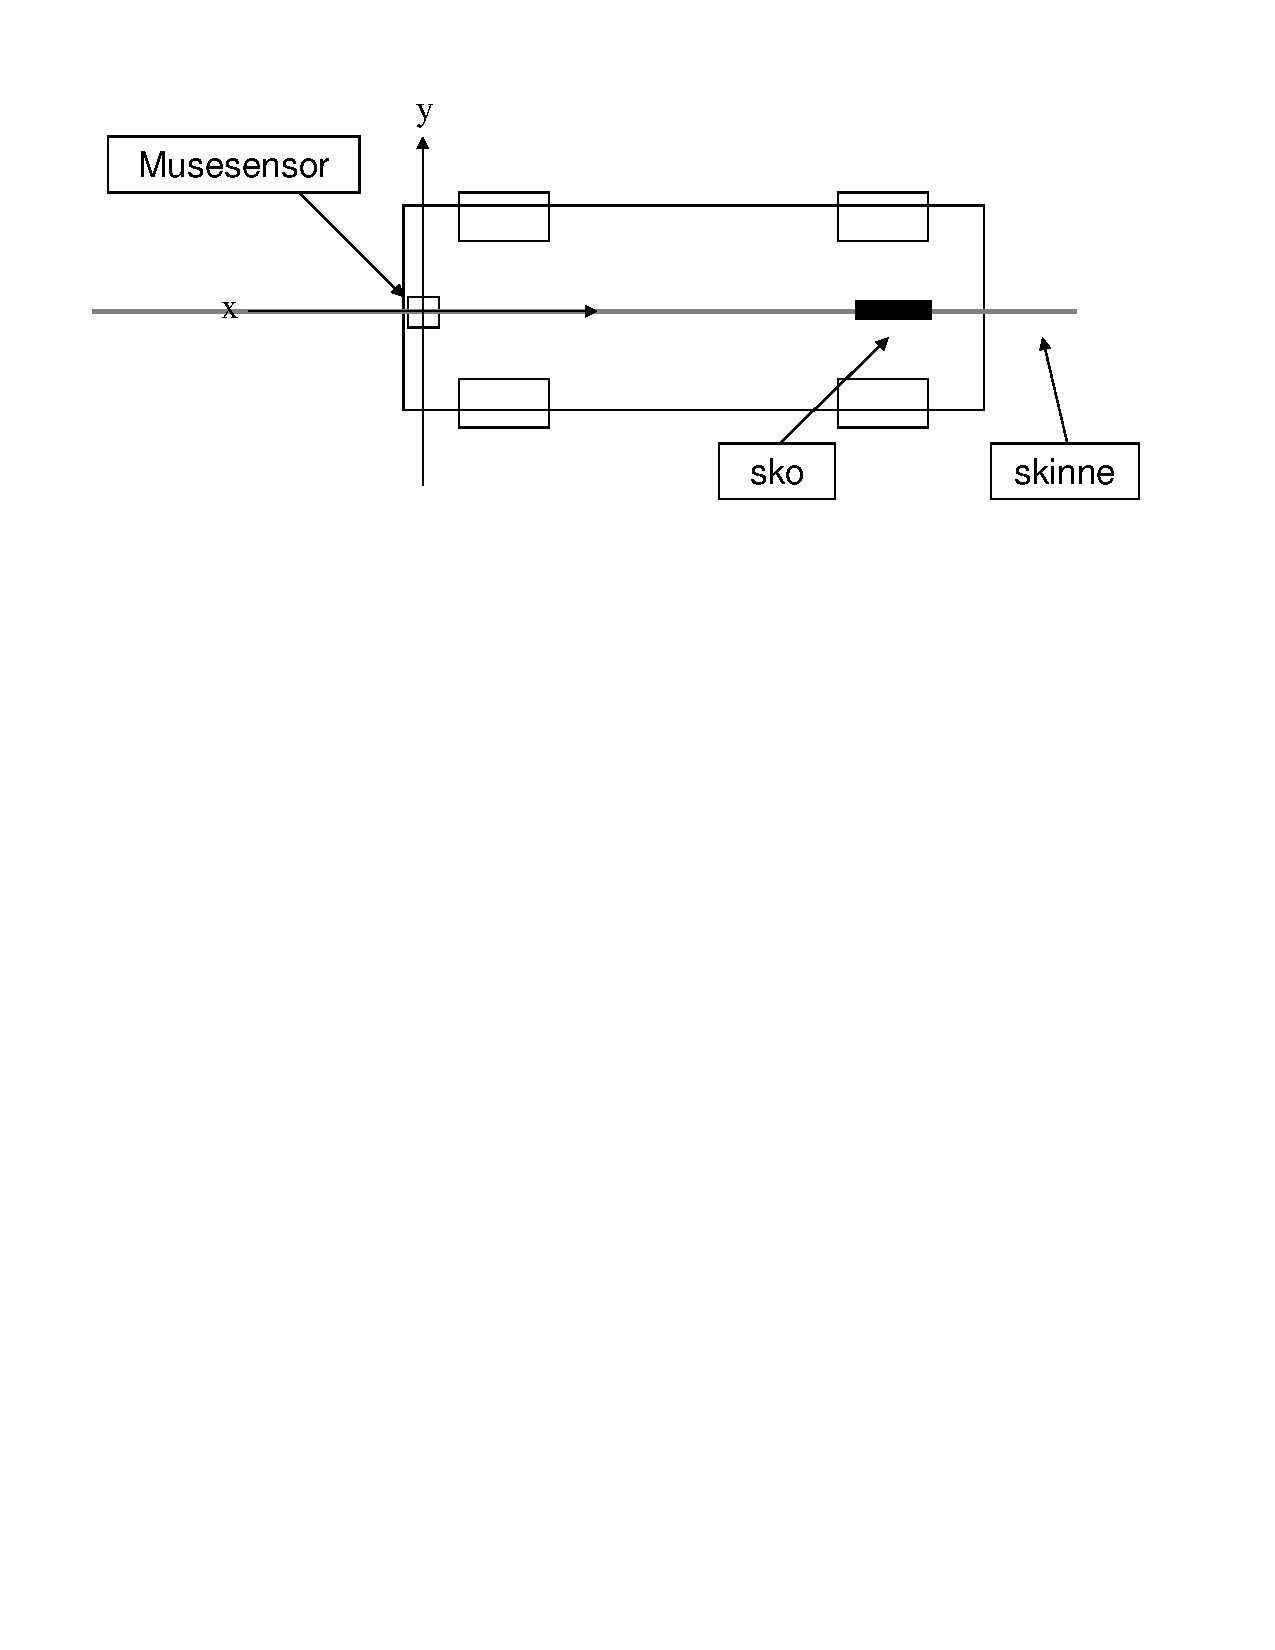
\includegraphics[scale=0.42,trim=50 500 70 20]{msligeud.pdf}}  %trim=l b r t
  \subfloat[Sving]{\label{fig:sving}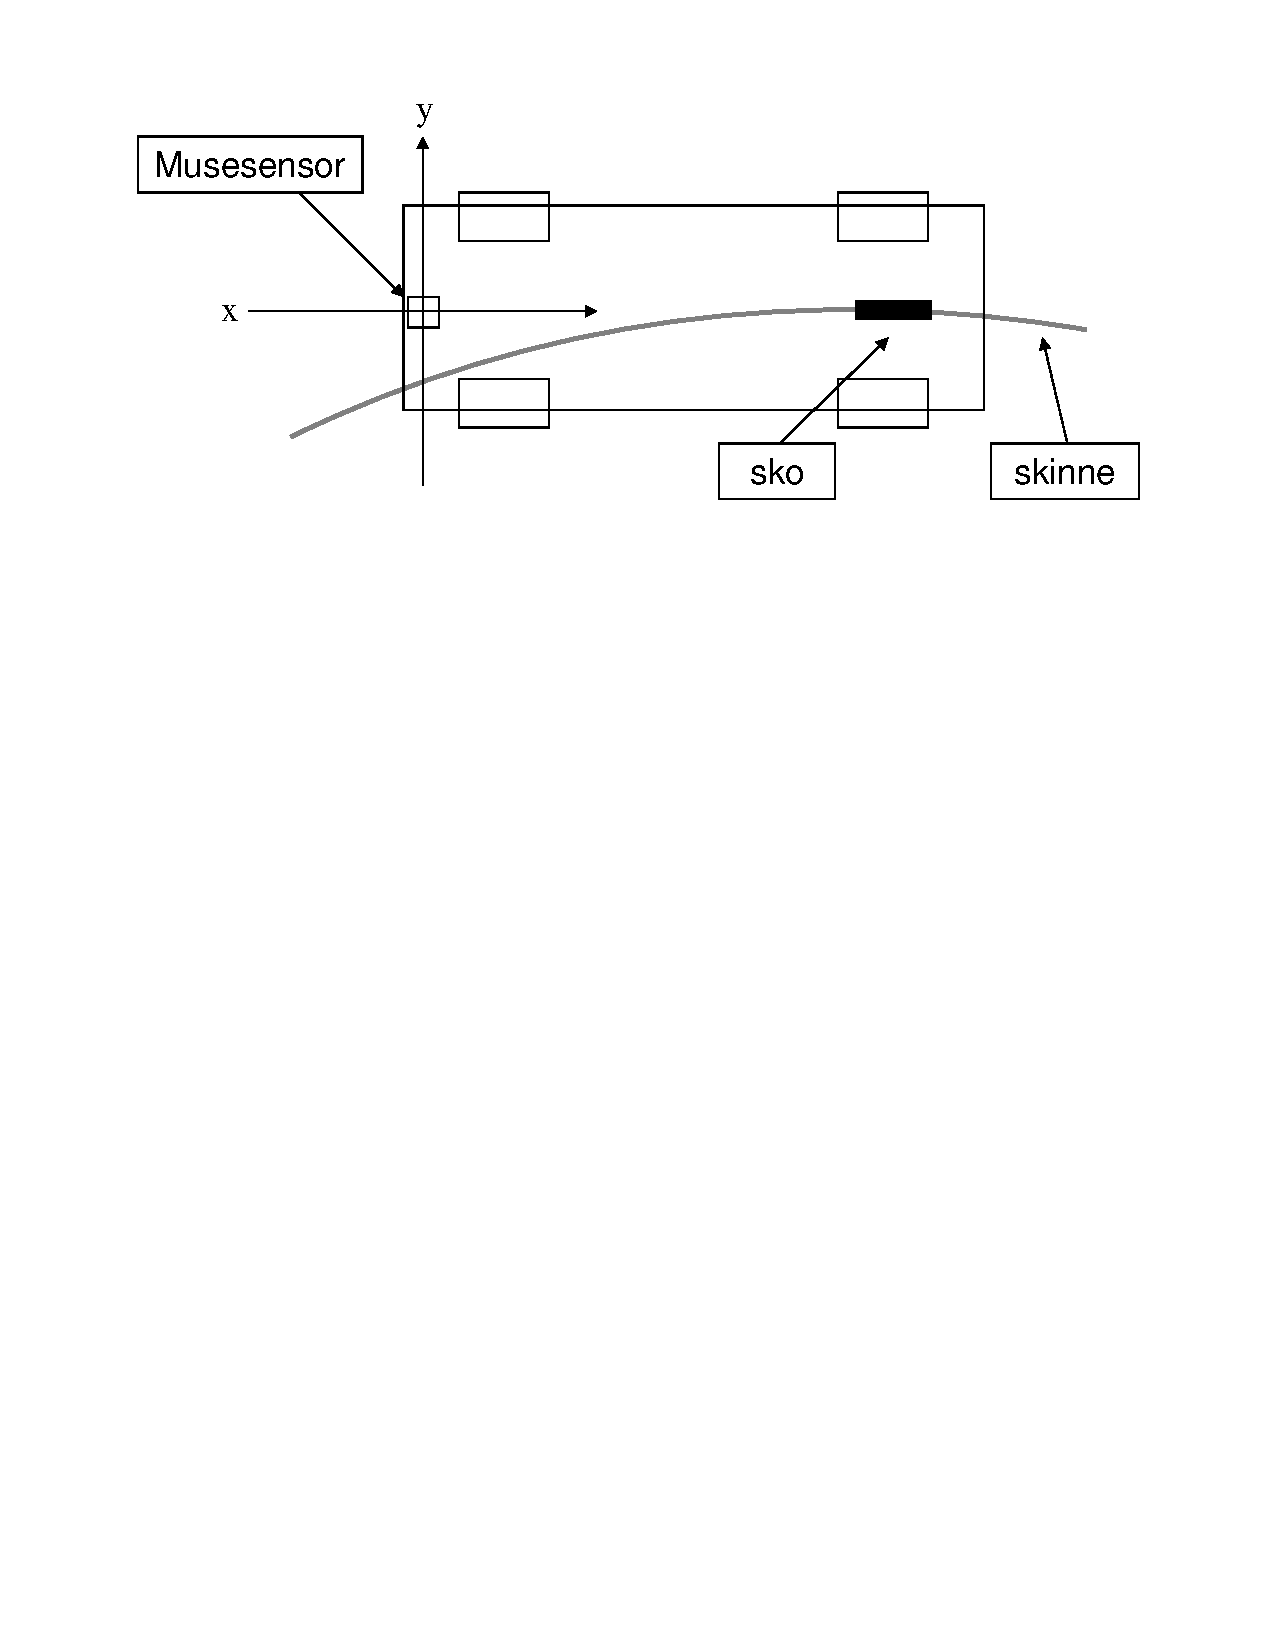
\includegraphics[scale=0.42,trim=80 500 70 20]{mssving.pdf}}
  \caption{Musesensorplacering}
  \label{fig:musesensor}
\end{figure}

\subsubsection*{Potentiometer p� sko}
Bilen er forsynet med en sko, der har forbindelse til to str�mf�rende skinner i banen. Skoen er af praktiske grunde lavet, s� den kan rotere i forhold til bilen.
N�r bilen k�rer ind i et sving, vil skoen dreje for at f�lge banens forl�b. Ved at montere et drejepotentiometer mellem skoen og bilen, er det muligt at opfange denne rotation. Konstruktionen er umiddelbart simpel, men �get friktion fra potentiometeret vil h�mme skoens bev�gelsesfrihed og dermed �ge bilens friktion i det den svinger.

\subsubsection{Detektering af m�lstreg}
Der er valgt en optocoupler til detektering af m�lstreg. Ingen andre alternativer blev overvejet til dette form�l.
\subsection{Valgte sensorer}
Til m�ling af hastighed og afstand, er musesensoren valgt. Den er valgt fordi den forventes at give den bedste pr�cision, og det er en direkte m�ling af bilens bev�gelse i forhold til banen. En musesensor er mere kr�vende og kompliceret at konstruere end nogle af de andre alternativer. Selvom dette er en ekstra udfordring, anses det som en overskuelig l�sning. 

Til at registrere sving er valget faldet p� et accelerometer. Der vil kunne registreres udslag p� accelerometeret, s� snart bilen k�rer ind i et sving, hvor den bliver udsat for centripetalaccelerationen.

Det eneste bud p� en sensor til detektering af m�lstregen er optocoupleren, hvorfor den er valgt.


\newpage
\section{Hardware}
I denne sektion beskrives, i detajler, de sensorer, der bruges i Scalextricbilen. Hver sensor vil blive beskrevet for sig og har hver sit eget kredsl�b og tilslutning ATmega32 microcontrolleren.

Ved projektstart samledes et, i forvejen designet, print hvorp� ATmega32 microcontrolleren, et bluetooth kommunikationsmodul og stik til interfacing af sensorkredsl�b er monteret. Al elektronik beskrevet i l�bet af dette afsnit er lavet som moduler, der er tilsluttet ''hovedprintet'', hvorp� microcontrolleren sidder.

\subsection{Microcontroller}
I projektet benyttes en AVR ATmega32 microcontroller som samlingspunkt for sensorinput og til signalbehandling. Den styrer ligeledes motorhastighed og retning. Her beskrives kort, hvordan microcontrolleren er bygget op og hvilke funktioner - af dem der bliver udnyttet i dette projekt - den indeholder.

ATmega32 er en 8-bit microcontroller, der bygger p� RISC\footnote{Reduced Instruction Set Computing} designstrukturen, hvilket kort sagt betyder, at microcontrollerens instruktioner alle er forholdsvis simple og kun tager kort tid (mange kun 1 \textit{clock cycle\footnote{Tiden mellem �n stigende flanke til den n�ste stigende flanke p� et pulserende signal}}). ATmega32 microcontrolleren har 32kB programhukommelse, der ikke slettes, hvis str�mmen afbrydes og 2kB SRAM\footnote{Static random-access memory}, som ikke best�r hvis str�mmen afbrydes.

AVR microcontrolleren indeholder en lang r�kke periferiske enheder, hvoraf mange bliver brugt i forbindelse med kommunikation og input fra sensorer. Deriblandt er analog-til-digital konverteren, som kan ''overs�tte'' et analogt signal til en digital, bin�r, v�rdi i op til 10-bit opl�sning. Der benyttes ogs� en analog komparator, som funktionelt ligner et almindeligt komparatorkredsl�b (op-amp med positiv feedback). Der kan frit v�lges referencesp�nding til komparatoren - alts� den sp�nding indgangssignal sammenlignes med - mellem enten en intern 2,56 V eller en ekstern sp�nding p�f�rt en indgang.

SPI\footnote{Serial Peripheral Interface} og USART\footnote{Universal synchronous/asynchronous receiver and transmitter} er begge enheder til seriel kommunikation. De er ogs� i forvejen indbygget i ATmega32 og bliver beskrevet mere indg�ende i senere software afsnit.


\subsection{Accelerometer} 
N�r bilen er i et sving, bliver den accelereret ind mod centrum af svinget. Forudsat at svinget er j�vnt, vil sammenh�ngen mellem radius, hastighed og centripetalacceleration\footcite[70-72,124-128]{fysik} v�re:

\begin{align}
	a_{cen}=\frac{v^2}{r}
	\label{eq:centripetal}
\end{align}

N�r bilen er i opm�lingstilstand, er det derfor muligt at detektere sving ved hj�lp af et accelerometer. Til dette form�l er der valgt et accelerometer, ADXL203 fra Analog Devices, der kan m�le b�de dynamisk og statisk acceleration p� maksimalt $1,7g =16,7m/s^2$.
Hvis hastigheden er kendt, er det muligt at beregne radius af svinget og derved bestemme om bilen befinder sig i det indre- eller ydre spor:

\begin{align}
r=\frac{v^2}{a_{cen}}
\end{align}

Figur \ref{fig:indreydre} viser m�lt radius for det indre- og ydre spor.

\begin{figure}[htb]
  \centering
  \subfloat[Indre]{\label{fig:Indre}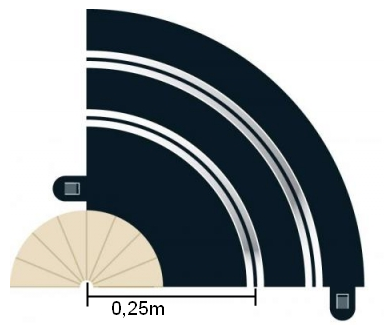
\includegraphics[scale=0.42]{radiusindre.png}}  %trim=l b r t
  \subfloat[Ydre]{\label{fig:ydre}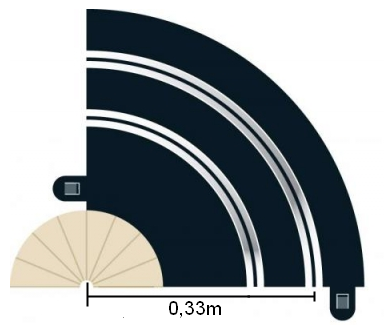
\includegraphics[scale=0.42]{radiusydre.png}}
  \caption{Radius for indre og ydre spor}
  \label{fig:indreydre}
\end{figure}

P� grund af accelerometerets begr�nsning p� $16,7m/s^2$, er den maksimale hastighed, bilen kan k�re i opm�lingstilstanden ved sving derfor:
I det indre spor: 

\begin{align*}
v=a_{cen}\cdot r_{indre}=16,7\cdot0,25m=2,0 m/s
\end{align*}

I det ydre spor:
\begin{align*}
v=a_{cen}\cdot r_{ydre}=16,7\cdot0,33=2,3 m/s
\end{align*}

Accelerometeret er placeret forrest i bilen, da bagenden kan skride ud og derved �ndre accelerometerets radius i forhold til svinget. Udskridning vil dog, uanset accelerometerets placering for�rsage, at accelerometeret bliver roteret i forhold til bev�gelsesretningen, og dermed ikke m�ler vinkelret p� denne - hvilket vil give en lille fejl.

\subsubsection{Kredsl�b til Accelerometer}
Forsyningen til accelerometeret er afkoblet med en 0,1$\mu$F kondensator (se figur \ref{fig:acc_print}), for at minimere st�j. Kondensatoren mellem udgangen og stel bestemmer b�ndbredden. Da det er relativt langsomme �ndringer, der skal m�les, kan st�j reduceres yderligere, ved at v�lge en lav b�ndbredde. I bilen anvendes en kondensator p� $1\mu$F (se Appendiks \ref{sec:bilag_acc}) og b�ndbredden bliver da 5Hz. Accelerometeret er forbundet til ATmega32 microcontrolleren gennem port AD0.

\begin{figure}[htb]
	\begin{center}
	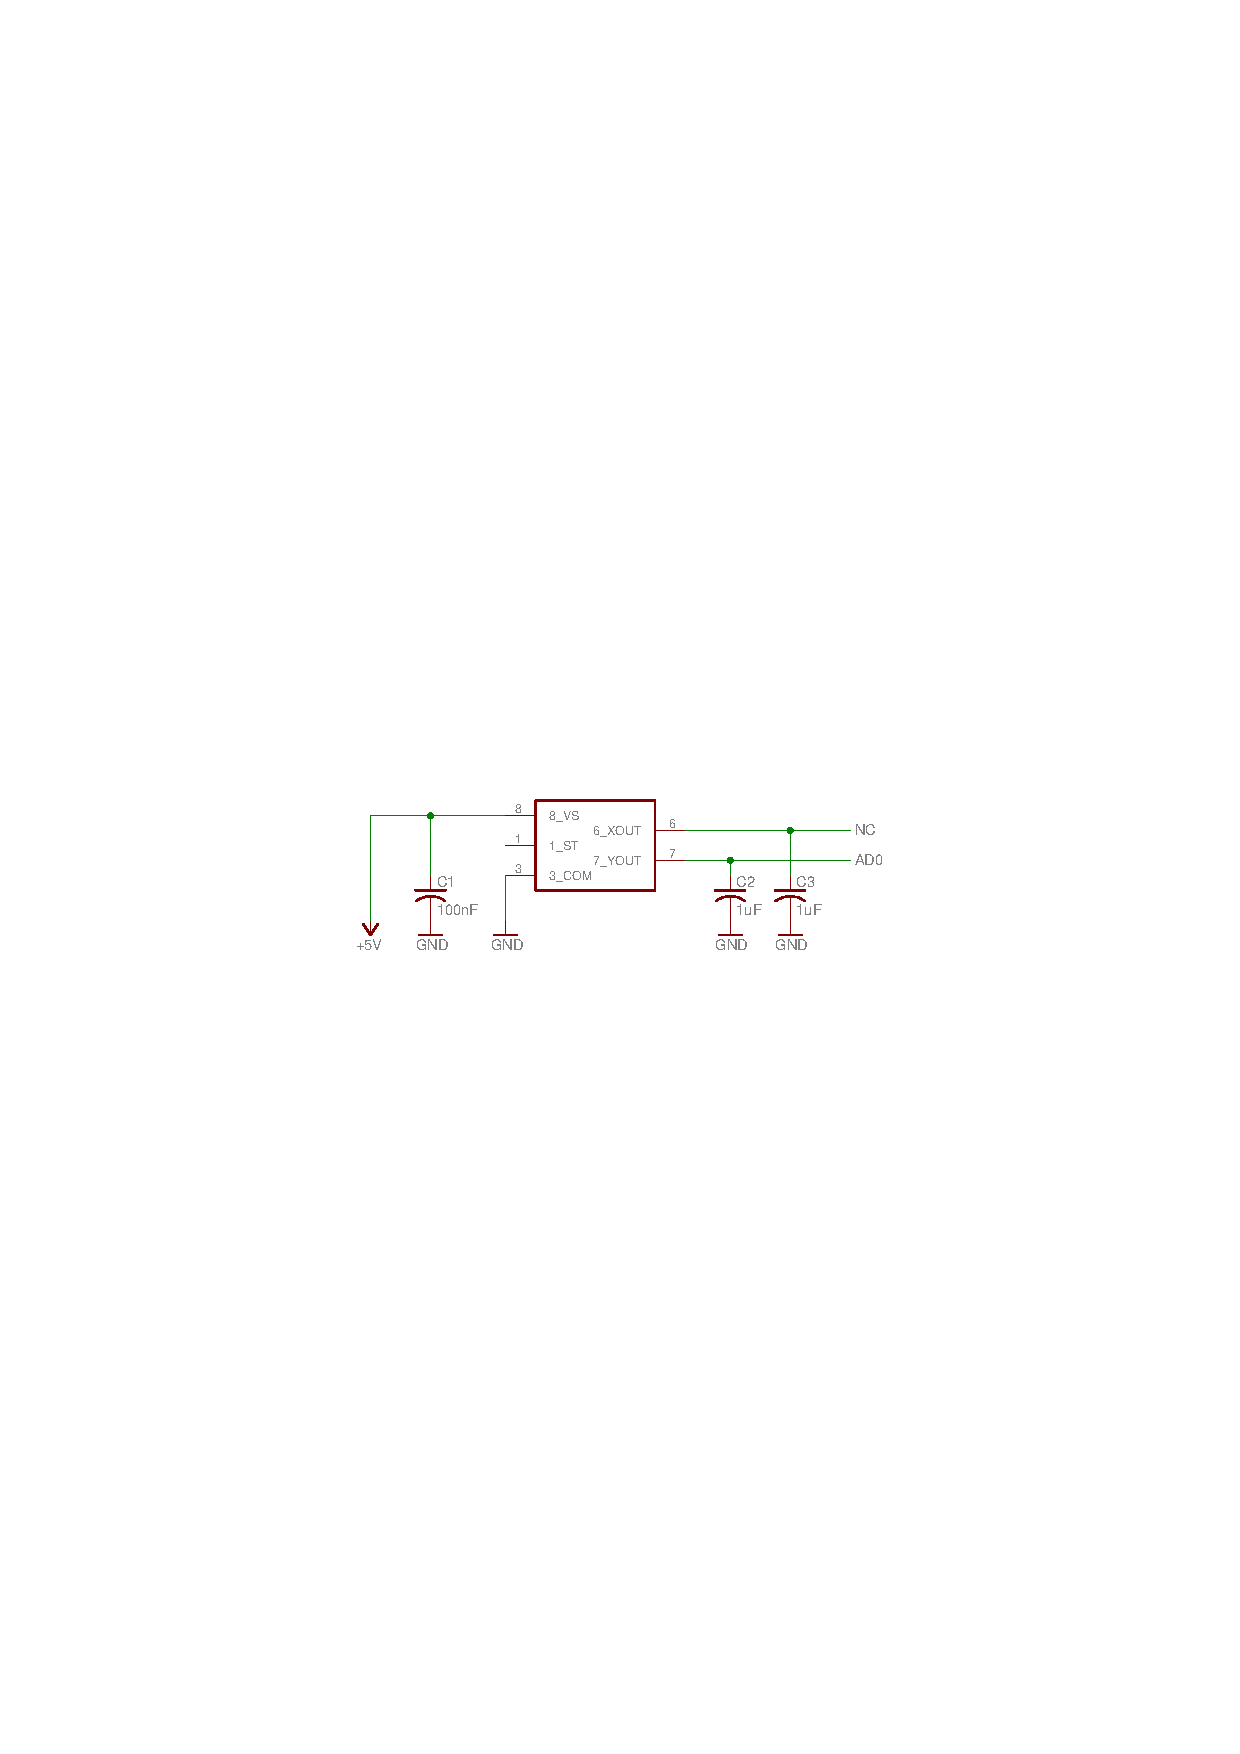
\includegraphics[scale=1.08,trim=200 380 200 380]{accelerometer_v1.pdf}%trim=l b r t
	\caption{Accelerometerdiagram}
	\label{fig:acc_print}
	\end{center}
\end{figure}

\subsubsection{AD konvertering}
AD-converterens reference er tilsluttet til en 5V forsyning. Det betyder at 5V svarer til en v�rdi p� 1023, hvilket ogs� kaldes 5V fullscale. Det vurderes, at en 8 bit opl�sning er tilstr�kkelig, og da det er nemmere at h�ndtere 8bit internt i processoren, v�lges en opl�sning p� 8bit fremfor 10bit. Da accelerometeret er begr�nset til $16,7m/s^2$ kan det kun give et udslag fra 0,8V til 4,2V. Ved en 8 bit pr�cision er der $5/256 V/bit$. Accelerometeret leverer $1 V/9,82 m/s^2$, hvor nulpunktet ligger p� $2,5 V$, i et omr�de fra $0,8 V$ til $4,2 V$. Ud fra dette er det muligt at beregne, hvor stor accelerationen pr. bit er:

\begin{align*}
\frac{9,82 m/s^2}{1V}\cdot\frac{5V}{256bit}=0,192\frac{m/s^2}{bit}
\end{align*}

Det vurderes, at det er muligt at k�re 1m/s i svinget uden at bilen falder af banen. Dette vil teoretisk give et udslag p� 

\begin{align*}
	\frac{v^{2}}{r\cdot 0,192\frac{m/s^2}{bit}}=bit
\end{align*}
Indre spor:
\begin{align*}
	\frac{1^{2}}{0.25\cdot 0,192\frac{m/s^2}{bit}}\approx\pm21 bit
\end{align*}
Ydre spor:
\begin{align*}
	\frac{1^{2}}{0.33\cdot 0,192\frac{m/s^2}{bit}}\approx\pm16 bit
\end{align*}

Fordi der er et teoretisk udslag p� omkring 16 bit ved k�rsel i yderbane, vurderes det at 8bit opl�sning er tilstr�kkelig til at detektere sving.
\subsection{Optocoupler}
Halvlederbaserede komponenter s�som dioder og transistorer reagerer p� lys i det synlige spektre og i s�rdeleshed infrar�dt lys, hvis indkapslingen er gennemsigtig.

N-lag materiale laves ved at forurene halvlederen med et grundstof fra hovedgruppe 5. Det kendetegnes ved, at der er nogle f� frie elektroner, og at det er en rimelig god elektrisk leder. P-lag materiale laves ved at dupe halvlederen med et grundstof fra hovedgruppe 3. Her er der et underskud af elektroner eller et overskud af ''huller''. P-lag er ligeledes en rimelig leder.

N�r en NP overgang belyses, dannes der elektron-hulpar ved hj�lp af den fotovoltaiske effekt, og det forsager, at der l�ber en str�m $I_{lum}$ fra N til P laget. Str�mmen stiger proportionalt med lysstyrken. Dette princip udnyttes i solceller - se figur \ref{fig:np}a.

Hvis der p�trykkes en positiv sp�nding over NP overgangen, vil der l�be en meget lille str�m $I_{sat}$ fra N til P, dette reducerer responstiden n�r NP overgangen belyses vil $I_{lum}$ stort set v�re u�ndret se figur \ref{fig:np}b.

\begin{figure}[htb]
	\begin{center}
	\subfloat[NP lag]{
	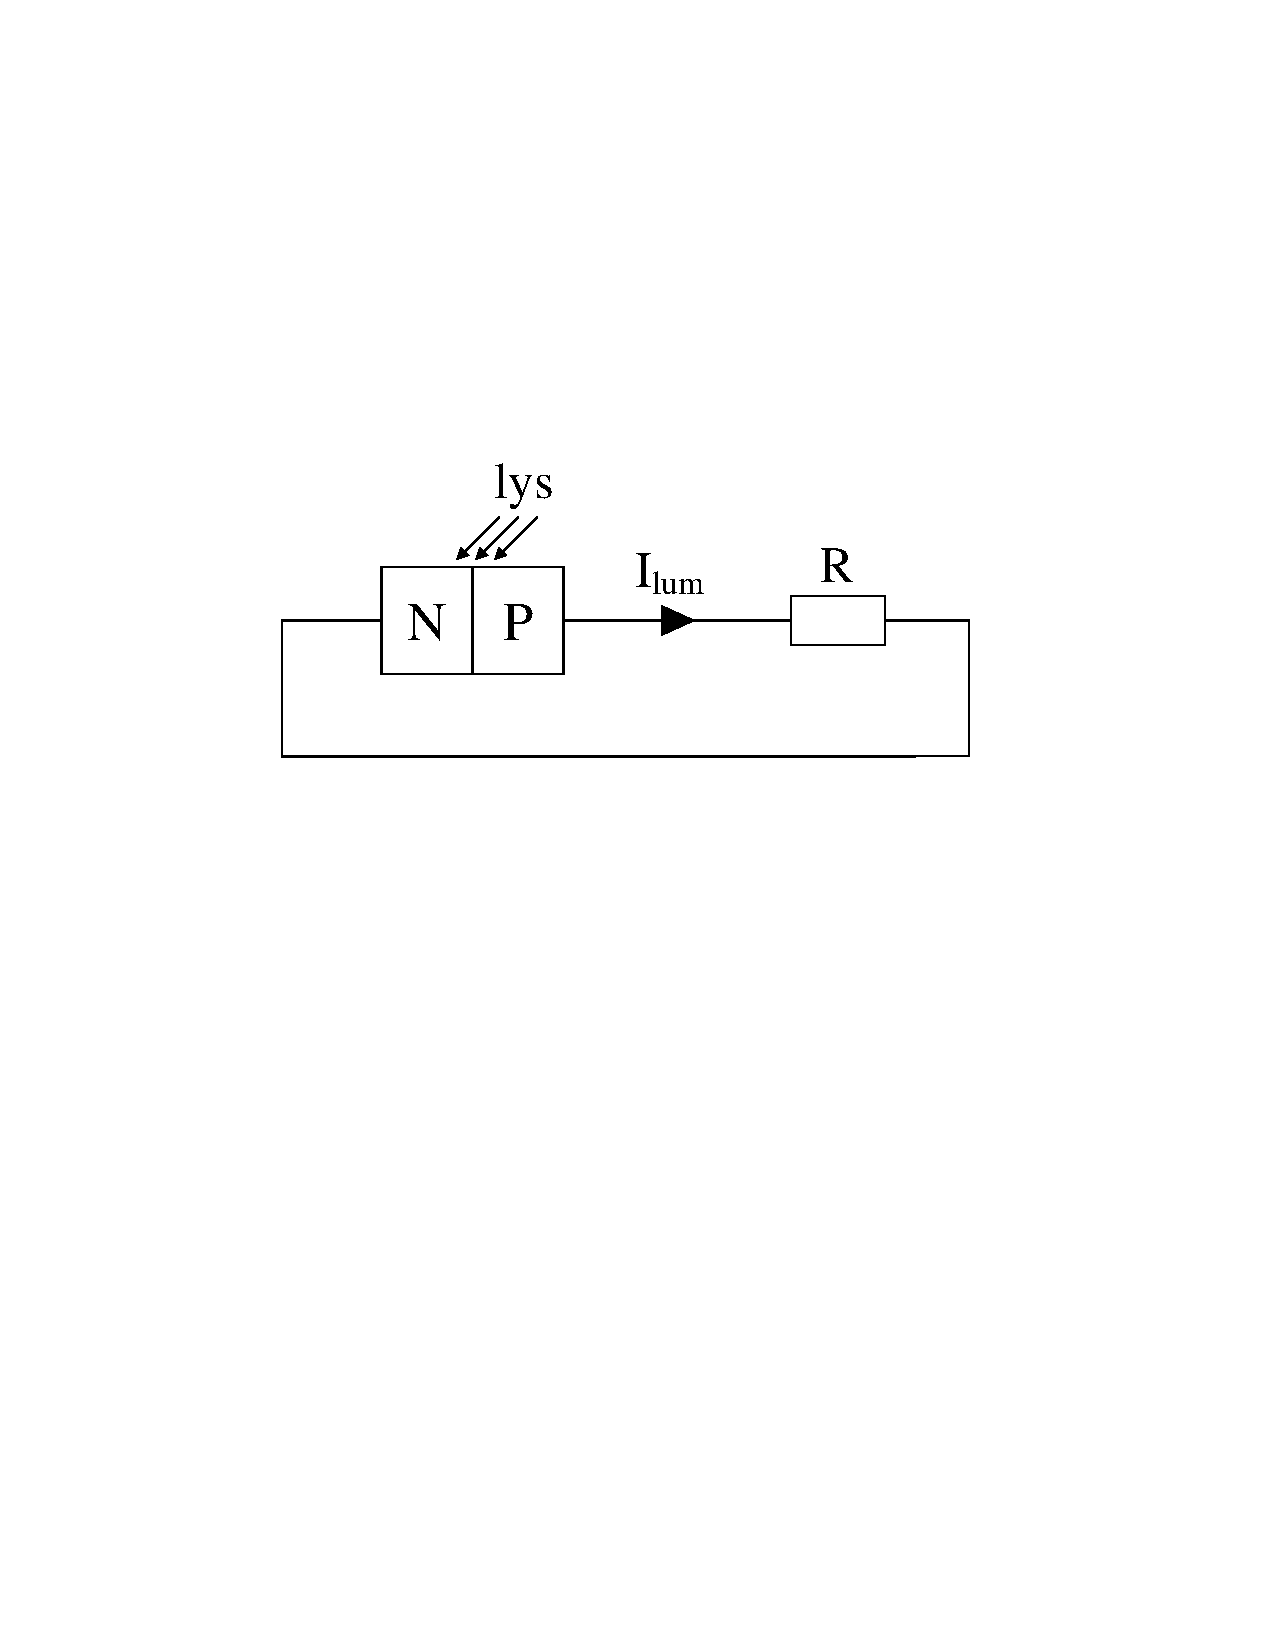
\includegraphics[scale=0.42,trim=150 425 100 200]{np.pdf}}%trim=l b r t
	\subfloat[NP overgang p�trykket positiv sp�nding]{
	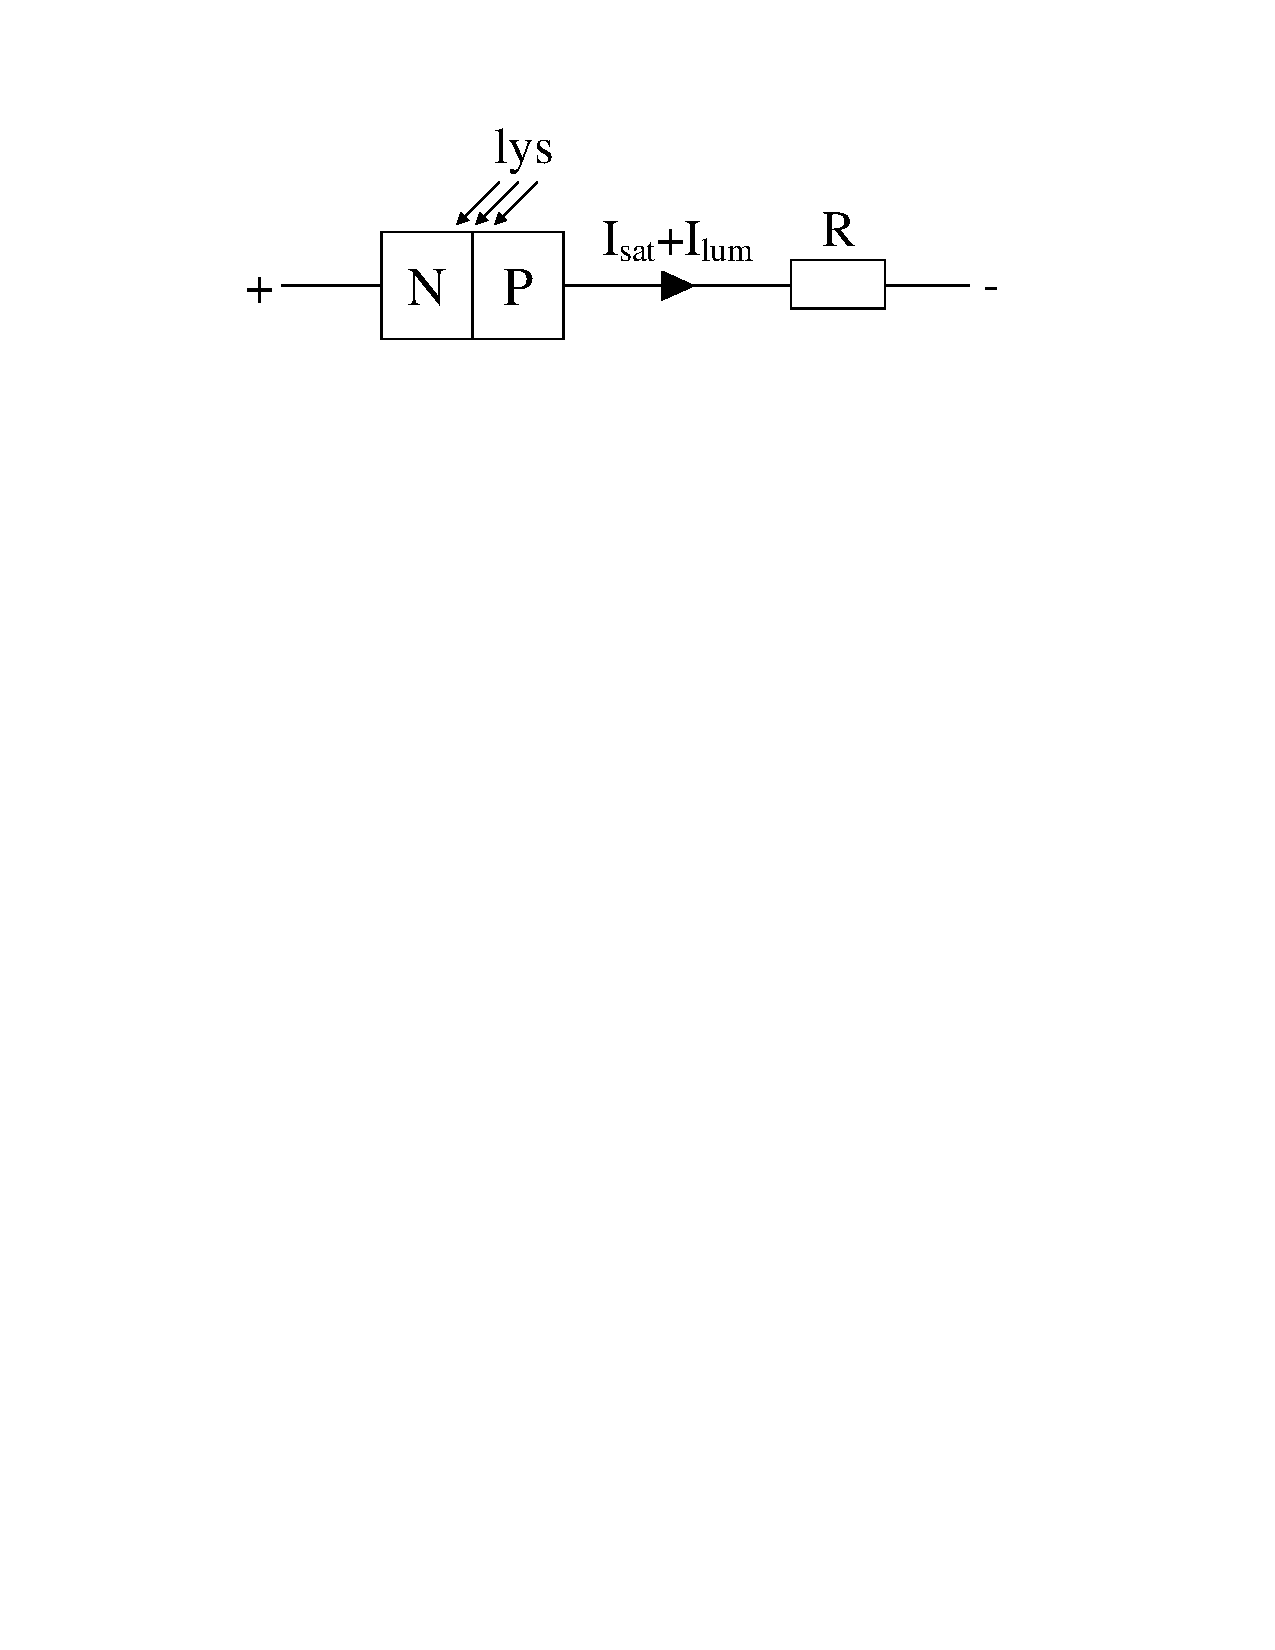
\includegraphics[scale=0.42,trim=100 625 100 50]{np_for.pdf}}%trim=l b r t
	\caption{NP lag}
	\label{fig:np}
	\end{center}
\end{figure}

En fototransistor er en modificeret transistor, hvor en del af komponenten kan belyses. Producenterne har v�ret s�rligt opm�rksomme p� at fremme lysf�lsomhed ofte ved at montere en linse eller lignende. Fototransistorrespons er st�rst i det infrar�de omr�de, derfor benyttes der ofte en infrar�d diode som lyskilde.

Der er valgt at bruge en optisk sensor fra Vishay semiconductors, model CNY70. Dette er en optisk sensor med et transistoroutput. Sensoren best�r en af diode og en NPN fototransistor. Dioden udsender infrar�dt lys, med en b�lgel�ngde p� 955nm. En NPN transistor best�r af to N-lag og et p-lag som vist p� figur \ref{fig:npntrans1}.

\begin{figure}[htb]
	\begin{center}
	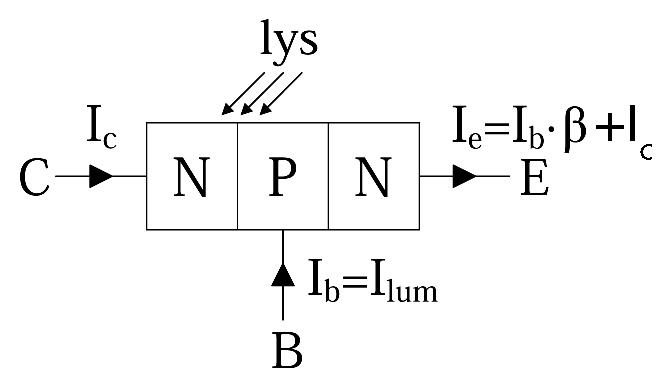
\includegraphics[scale=0.46,trim=0 0 0 0]{npn_trans.pdf}%trim=l b r t
	\caption{NPN fototransistor}
	\label{fig:npntrans1}
	\end{center}
\end{figure}

N�r der p�trykkes en positiv sp�nding over collector og emitter benene vil NP overgangen mellem collector og base ogs� blive p�trykket en positiv sp�nding. Hvis denne overgang belyses, vil der l�be en str�m $I_{lum}$, der p� samme m�de som base str�mmen $I_{b}$ i en almindelig transistor vil styre, hvor stor en str�m der l�ber gennem transistoren. Derved bliver transistoren styret af, hvor stor en del af det infrar�de lys dioden udsender, der bliver reflekteret af den overflade, sensoren befinder sig over.

Optosensoren er forbundet som vist p� figur \ref{fig:fotosch}. R1 styrer, hvor stor str�m der l�ber i gemmen dioden. Hvis der regnes med et sp�ndingsfald over dioden p� $1,25V$ er der sp�ndingsfald p� $3,75V$ over R1. $3,75V/180ohm$ det giver en str�m p� $I=21mA$ gennem dioden.

\begin{figure}[htb]
	\begin{center}
	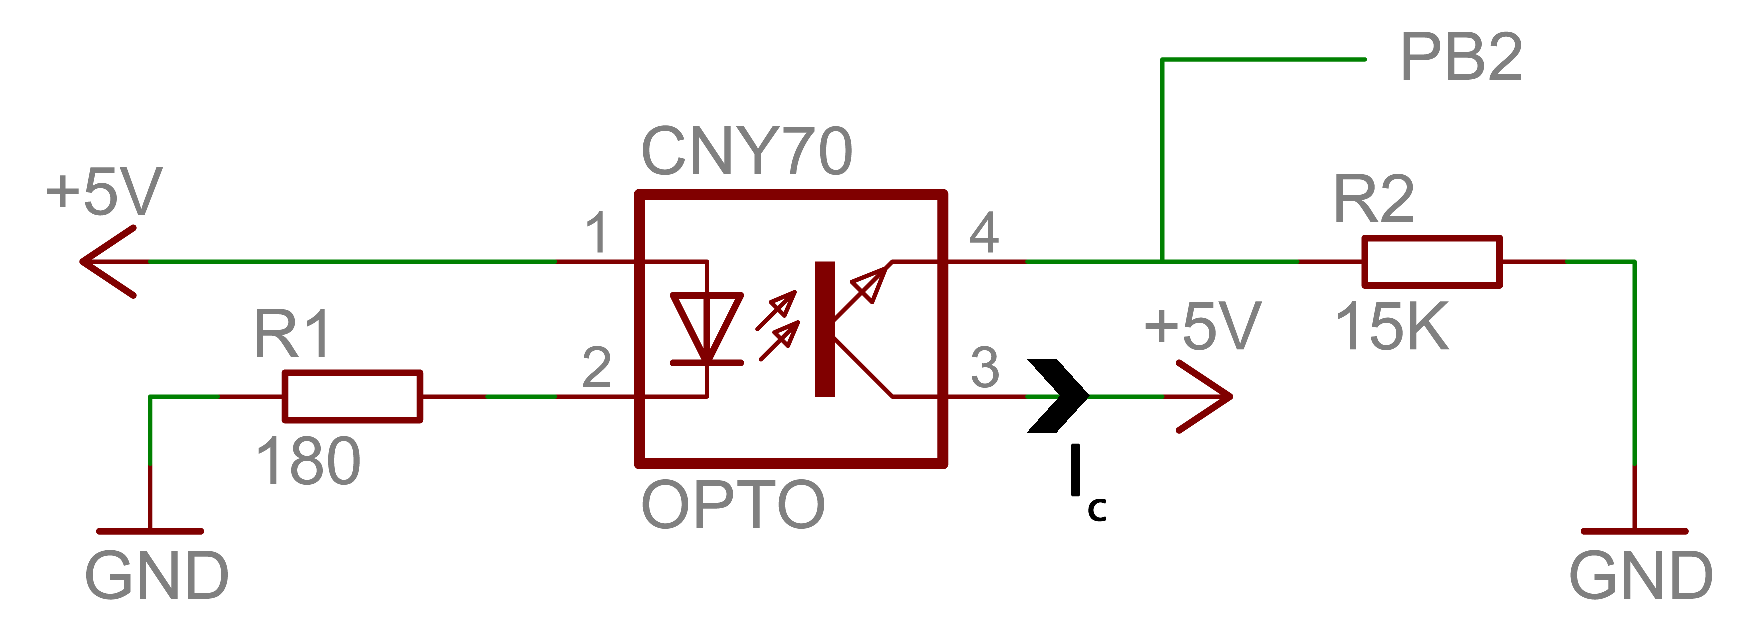
\includegraphics[scale=0.34,trim=0 0 0 0]{optosch.pdf}%trim=l b r t
	\caption{Fotosensorkredsl�b}
	\label{fig:fotosch}
	\end{center}
\end{figure}

Transistorens arbejdslinje vil i dette kredsl�b v�re:

\begin{align}
I_{C}=\frac{1}{R2}\cdot V_{CE} - \frac{V_{DC}}{R2}
\end{align}
Optosensoren er koblet til ATmega32 chippens komparator gennem port PB2, referencesp�ndingen er koblet til PB3. Ved at �ndre referencesp�ndingen er det muligt at justere hvorn�r optosensoren for�rsager et interrupt.

%/*
%Musesensor
% - Indledning
%Til at bestemme positionen af bilen,
% For at bestemme den n�jagtige position af bilen I forhold til banens start, er der arbejdet med den
%
%
%de teknikker en moderne computermus benytter sig af for at kunne afl�se sin position.
%
%Til at bestemme bilen hastighed, er der under bilen monteret en ADNS-9500 mussesensor. Sensoren kan l�bende afl�ses af bilen microcontroler for �ndringer I positionen af sensoren I forhold til overfladen under bilen. Ved en kontinuerlig afl�sning med fast tidsinterval af sensoren, repr�senterer den afl�ste v�rdi direkte hastigheden af bilen, og ved at summere alle 
%
%\begin{table}[htb]
%	\begin{center}
%	\begin{tabular}{l|l|l}
%	
%	Sensor				 & Max hastighed			& Max accelleration		& Teknologi		\\
%	\hline
%	ADNK-2080				& 30ips				& 20g 				& LED
%	ADNS-9500 				& 200ips 				& 30g				& Laser\\
%
%
%	\end{tabular}
%	\end{center}
%	\caption{Telegramkommandoer}
%	\label{tab:kommandoer} %%ref
%\end{table}
%
%
%Eventuelt lidt om hvordan de virkede f�r laser.
%- Forklaring af hvordan den tager billeder af overfladen og sammenligner.
% - Valg af sensor ud fra krav om hastighed <<<<<<<<<<<<<<<<<
%  (Billeder af hvordan laser og kamera er placeret i forhold til overfladen)
%  - Eventuelt henvisning til tidligere artikler omkring brug af musesensore til displacement messurement.
%  - (Hvorfor er den bedre?)
%  - Pr�cission
%  - Ul�mper
%
% - Kommunikations med den? Afl�sning af data fra sensoren
% - Circle of life
%; Metoder til afl�sning / timings
%
%
%Til forskel fra en almingelig RS232 seriel kommunkation, er der ved SPI f�lles clock som sendes fra MASTER enheden.
%
%   - Hastighed p� SPI?
%Beregninger
%Timings p� ADNS sensor
%  - Hvad kan den fort�lle tilbage omkring position (Og hvad kan den ikke)
%   - Tegninger over SPI hardware interface.
%   - / Tilslutnig til ATmega32A
%  - SPI p� atmega32A
%   - Registre
%   - Interupts
% - ASM kode til opsamling af data fra sensoren.
%  - Forskellige modeller for opsamling og behandling af data.
% - Montering p� bilen
%  - Forklaring af hvad det er den kan se n�r vi f�r en dX eller dY.
%
% TEST AF SENSOR
%  - Hvor gode data f�r vi?
%LASEREN (B�lgel�ngde, 
%
%Tegninger/Figurer:
%Indre og yderebane (Se tavle) OK
%Billeder af bilen fra oven (Skal bruges til visning af placering af sensoren) --  er Niels ved at lave dette?
%
%
%
%*/
\subsection{ADNS Sensor}
En essentiel faktor for at opn� den hurtigste omgangstid p� Scalextricbanen, s�vel som p� en almindelig racerbane er, at bremse ned til svinget p� det helt rigtige tidspunkt og holde den hurtigst mulige hastighed hele svinget igennem. Ved en for sen nedbremsning vil bilen have en for h�j hastighed i svinget og k�rer derfor af banen. Modsat vil en for tidlig nedbremsning, i forhold til svinget betyde, at man f�r en d�rligere omgangstid og derved neds�tter chancen for at vinde.

For at microcontrolleren skal vide, pr�cis, hvor p� banen bilen befinder sig, er der monteret en sensor fra en moderne computermus under bilen, da disse netop er i stand til at angive pr�cise positionsdata. Sensorens opgave er at m�le bilens bev�gelseshastighed i forhold til banen.

\subsubsection{Hvordan virker den?}
En moderne optisk mus er bygget op af en lyskilde, i form af en laser eller lysdiode, et kamera og en billedeprocessorenhed. Laseren er monteret s� den sidder forskudt i forhold til kameraet (se figur \ref{fig:adns_sideview}), og derfor vil skabe en masse sm� skygger i forhold til kameraets vinkling. Dette giver en bedre kontrast p� billedet fra kameraet, og derved bliver der flere unikke fikspunkter at m�le forskydelser i forhold til. Kameraet tager kontinuerligt billeder, og processorenheden regner p� billeddataen og finder fikspunkter i billedet. N�r sensoren flyttes i forhold til overfladen, vil disse fikspunkter flytte sig i forhold til billedet, optaget af kameraet. Denne information behandles i processoren, og udfra dette er den i stand til at beregne hvordan sensoren har flyttet sig i forhold til overfladen. Dog skal man v�re opm�rksom p�, at sensoren ikke er i stand til at afl�se rotation omkring sig selv.
%(SE FORSIDE AF DATABLAD UNDER THEORY OF OPERATION FOR INPUT TIL TEKST)

\begin{figure}[htb]
  \centering
  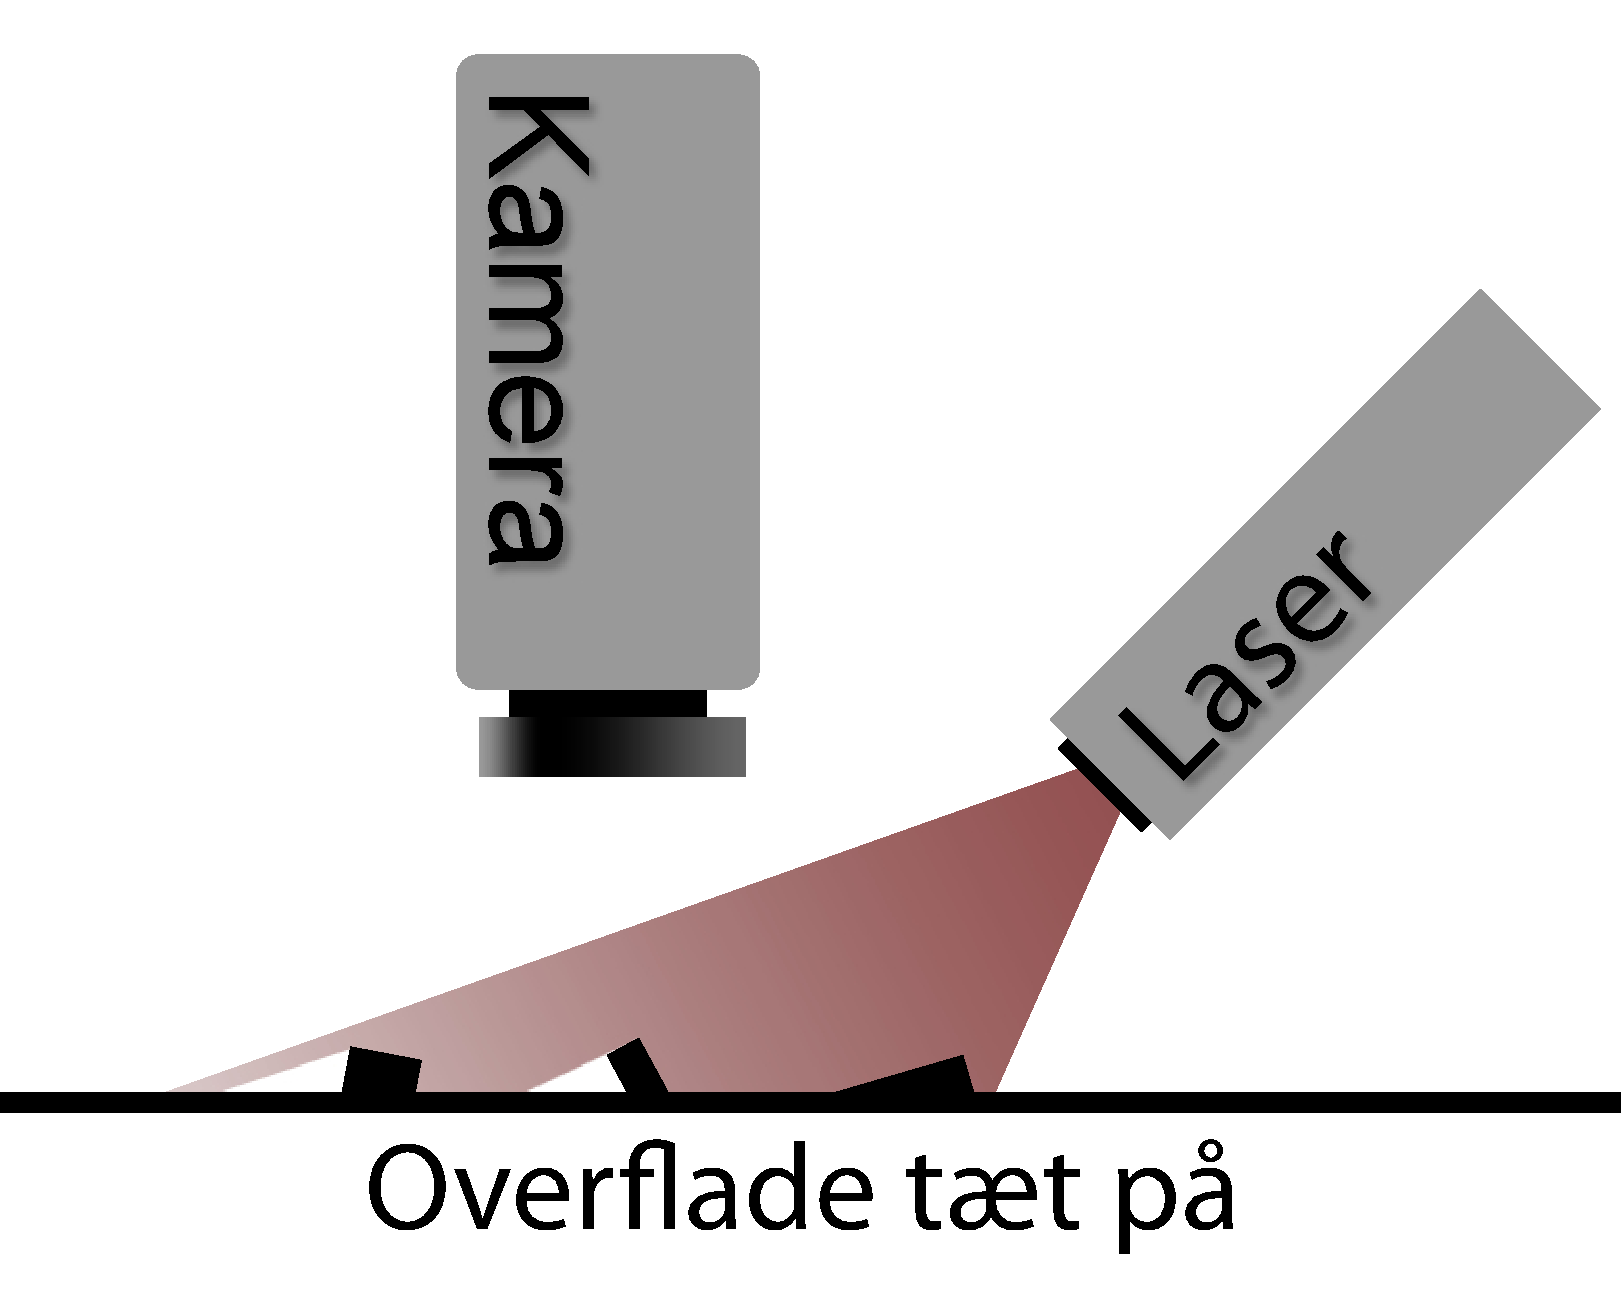
\includegraphics[scale=0.2]{ADNS_sideview.pdf}  
  \caption{ADNS sensor i forhold til overflade}
  \label{fig:adns_sideview}
\end{figure}

\subsubsection{Valg af musesensor} % Fordele ved den valgte sensor
Ved valg af sensoren er der lagt v�gt p�, at sensoren er i stand til at opfange positionsdata ved tilstr�kkeligt h�je bev�gelseshastigheder. F�r valget af sensor blev der derfor foretaget m�ling af bilens maksimale hastighed (se Appendiks \ref{sec:bilag_hastighed}), for at bestemme en minimumshastighed som sensoren b�r v�re i stand til at m�le. Konklusionen af hastighedsm�lingen blev, at sensoren skal v�re i stand til at afl�se hastigheder op til $5$ $\sfrac{m}{s}$.

Tidligere unders�gelser af optiske sensorer fra mus har vist, at disse har en h�j n�jagtighed. I en artikel\footcite{optimouse} fra 2003 er der beskrevet, hvordan en optisk mussensensor kan benyttes til 2D forskydelsesm�ling. De har p� det tidpunkt kunnet konkludere, at MSE\footnote{Mean square error} p� den afpr�vede sensor var mindre end $0,018$ $mm^{2}$ under optimale forhold.

Af lagerm�ssige grunde var det udelukkende Avago Technologies' sensorer der var mulige at fremskaffe til dette projekt, og denne producent oplyser ikke hvad man kan forvente af n�jagtighed p� deres sensorer, hvorfor denne faktor ikke kan tages med i valget af sensor. Det m� formodes, at resultatet fra tidligere n�vnte artikel er en god guideline, til hvilken pr�cision der kan forventes, og denne er langt bedre end, hvad der vurderes at v�re n�dvendigt.

De fleste musesensorer, der er kigget p�, er i stand til at registere accelerationer p� omkring $20$ $\sfrac{m}{s^{2}}$. 
Hvis bilen skal accelerere med $20$ $\sfrac{m}{s^{2}}$ til en makshastighed p� $5$ $\sfrac{m}{s}$ vil bilen opn� sin makshastighed p� $0,25$ $s$, s�fremt det antages at accelerationen er konstant. Ved at observere bilen k�re, ses det tydeligt, at dette ikke er tilf�ldet, og at denne faktor derfor ikke skal tages med i valget af sensor.

Kommunikationsinterfacet til Avago Technologies' musesensorer er enten TWI\footnote{Two Wire Interface} eller SPI\footnote{Serial Peripheral Interface}, hvilke ATmega32 microcontrolleren begge har hardwareunderst�ttelse for. S�ledes er dette heller ikke en afg�rende faktor for valget af sensor.

%(evt. tabel over valgmuligheder / udvalgte sensorer)
%Avago technologies tilbyder mange forskellige optiske mussesensore, baseret b�de p� LED og laser teknologi. 
Ved gennemgang af udvalget af sensorer, viser det sig at langt de fleste sensorer maksimalt kan m�le hastigheder op til $1-2$ $\sfrac{m}{s}$, og den eneste sensor, der er i stand til at m�le tilstr�kkeligt h�je hastigheder, er en ADNS-9500 sensor.
ADNS-9500 er en musesensor designet til professionelle computerspillere, der stiller h�je krav til n�jagtigheden af deres mus. Sensoren er i stand til at m�le hastigheder op til $5,08$ $\sfrac{m}{s}$ p� udvalgte overflader, og accellerationer op til $30$ $g$. Sensorens interne billedeenhed og processeringsenhed arbejder med op til 11750 billeder i sekundet, og laseren, der belyser overfladen, kr�ver ingen manuel justering og belyser overfladen med ikke synligt lys med en b�lgel�ngde p� omkring $832-865$ $nm$. Denne sensor blev valgt til projektet.

\subsubsection{Tilslutning af sensor}
Det er et krav, for at sensoren skal fungere optimalt, at der benyttes afkobling til alle forsyningsben p� kredsen. For at kunne have plads til denne afkobling under bilen, hvor sensoren er monteret, er der til form�let lavet et SMD\footnote{Surface mount devices} print. SMD printet indeholder den n�dvendige afkobling samt en transistor, som har til form�l at str�mbegr�nse den interne laser diode. Diagrammet til SMD printet er vist herunder p� figur \ref{fig:adns_sch}

\begin{figure}[htb]
  \centering
  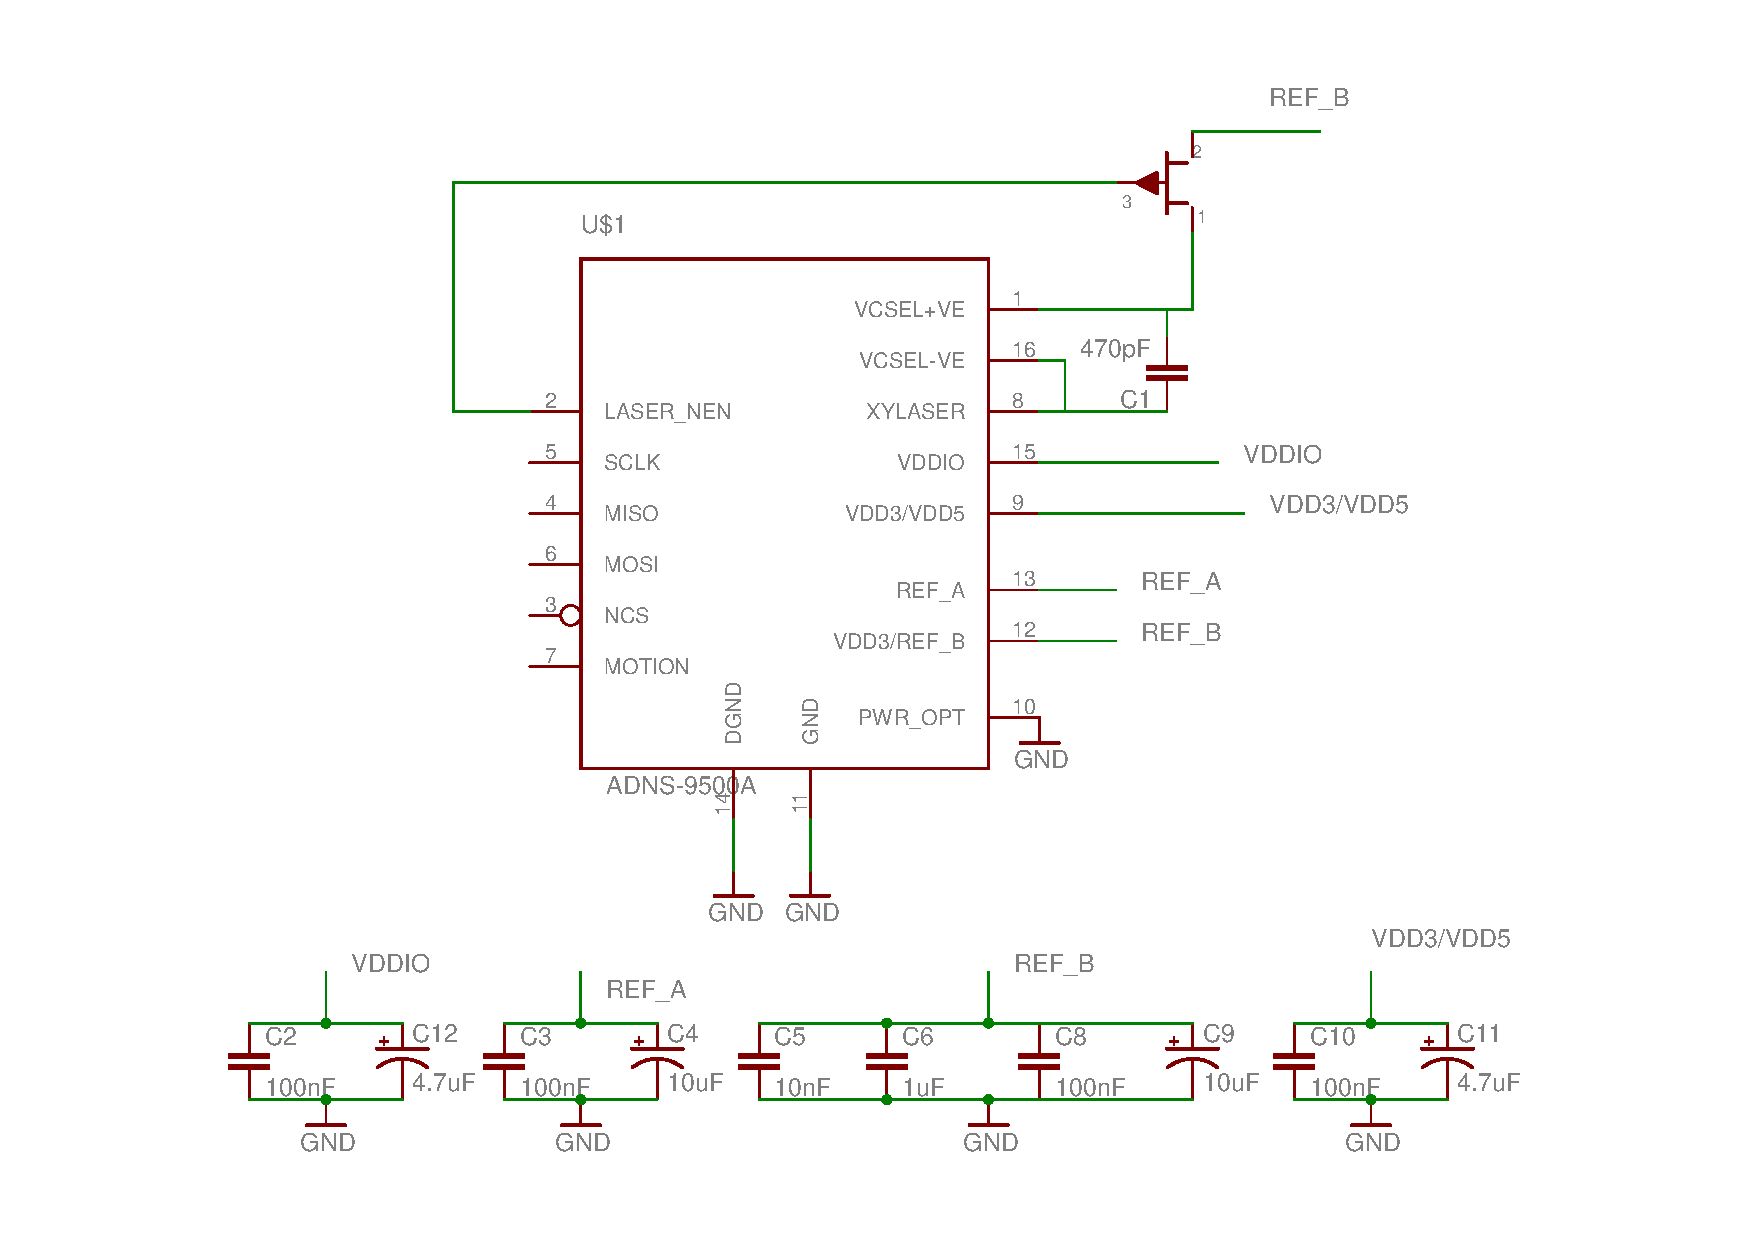
\includegraphics[scale=0.56,trim=50 8 50 30]{ADNS_sch.pdf}    %trim=l b r t
  \caption{ADNS sensor print}
  \label{fig:adns_sch}
\end{figure}
%\begin{figure}[htb]
%  \centering
%  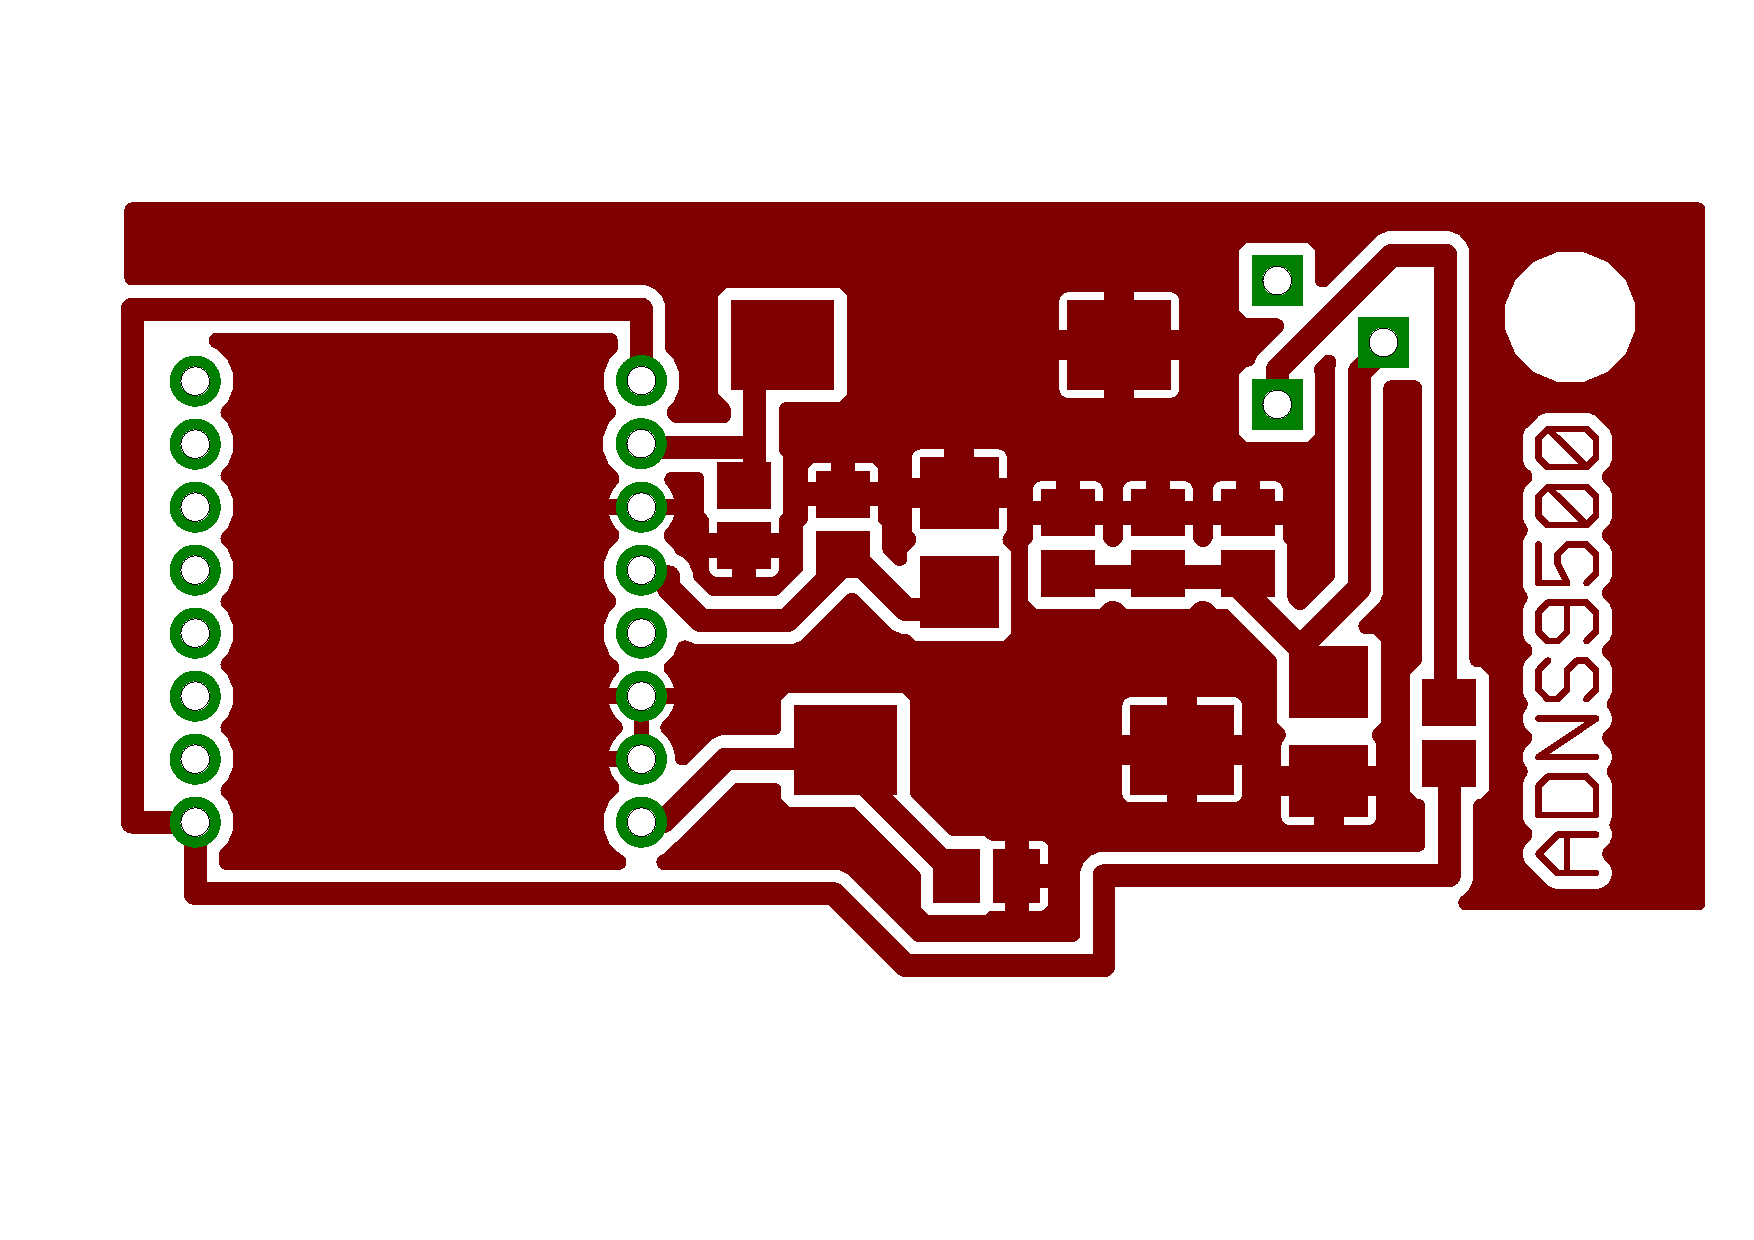
\includegraphics[scale=0.1]{ADNS_smd_front.pdf}  
%  \caption{ADNS print forside}
%  \label{fig:adns_smd_front}
%\end{figure}
%\begin{figure}[htb]
%  \centering
%  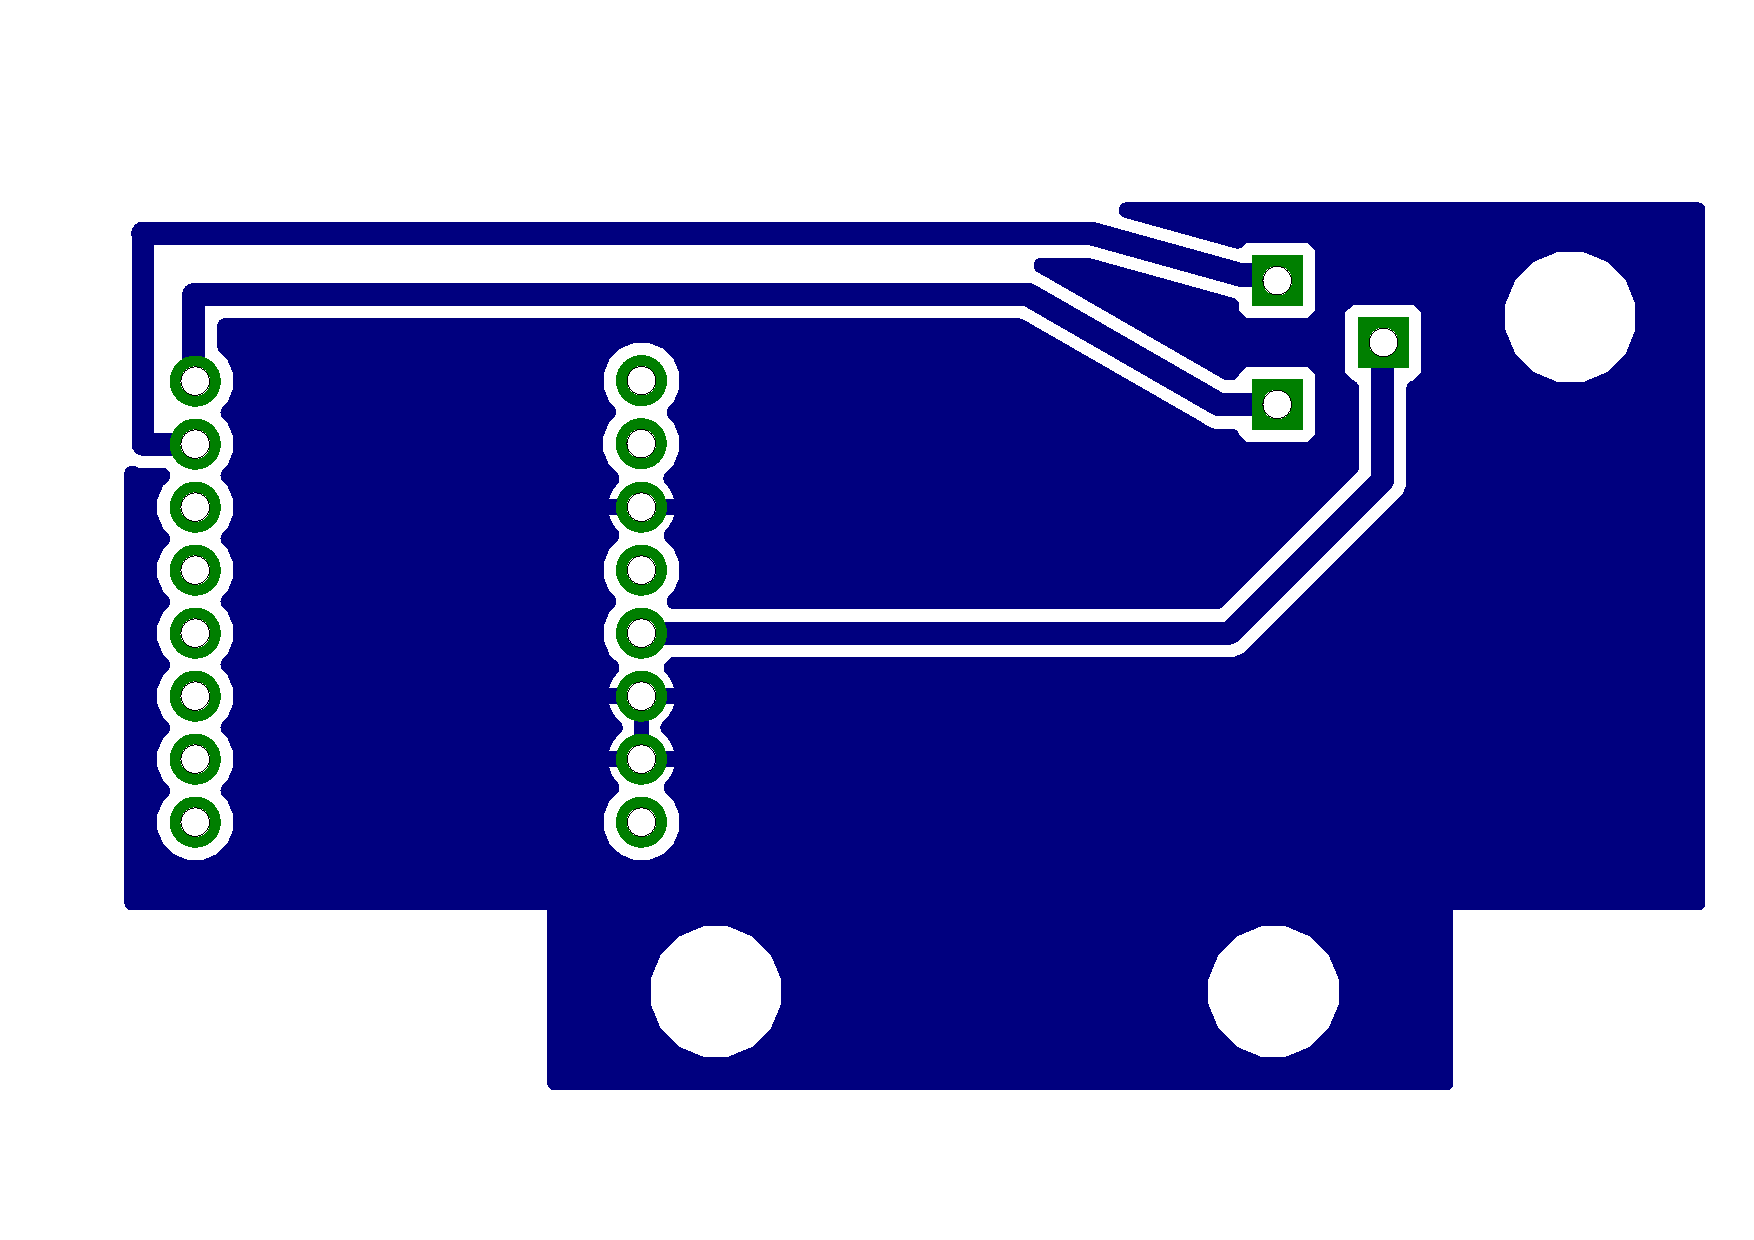
\includegraphics[scale=0.1]{ADNS_smd_back.pdf}  
%  \caption{ADNS print bagside}
%  \label{fig:adns_smd_back}
%\end{figure}
\subsubsection{Afl�sning af sensor}\label{sec:aflaesning_af_sensor}
ADNS-9500 sensoren kan udelukkende afl�ses ved hj�lp af SPI. SPI-protokollen er beskrevet senere, men det er vigtigt at v�re opm�rksom p�, at dataoverf�rslen foreg�r asynkront, og at dataen synkroniseres af en clockpuls, der er styret fra masterenheden, som i dette tilf�lde er ATmega32-controlleren.

%(Her skal ogs� st� noget omkring h�j og lav byte af hastighedsv�rdien fra sensoren)\\

Det betyder i praksis, at en l�sning af data fra sensoren kr�ver afsendelse af to bytes. F�rst sendes adressen der �nskes afl�st, hvorefter en tom byte sendes, mens dataen modtages. Den tomme byte er for, at ATmega32 microcontrolleren sender en clock til sensoren, som den kan sende data tilbage p�. %(SE FIGUR??)
Man kan v�lge kontinuerligt at sp�rge efter de v�rdier, man skal bruge fra sensoren, eller benytte sig af den indbygge mulighed for ''motion burst''.

Under udarbejdelsen af programkode til at afl�se sensoren er der vurderet fordele og ulemper ved de forskellige modeller for afl�sning, som gennemg�s i Appendiks \ref{sec:bilag_adnsaflaesning}. Herunder gennemg�s den valgte metode til afl�sning af sensor i detaljer. Konklusionen heraf blev, at benytte sensorens indbyggede motion burst kommando.

Ved motion burst sender man en kommando til sensoren, som herefter sender 14 bytes med data tilbage. De 14 bytes indeholder:

\begin{verbatim}
BYTE [00] = Motion
BYTE [01] = Observation
BYTE [02] = Delta_X_L
BYTE [03] = Delta_X_H
BYTE [04] = Delta_Y_L
BYTE [05] = Delta_Y_H
BYTE [06] = SQUAL
BYTE [07] = Pixel_Sum
BYTE [08] = Maximum_Pixel
BYTE [09] = Minimum_Pixel
BYTE [10] = Shutter_Upper
BYTE [11] = Shutter_Lower
BYTE [12] = Frame_Period_Upper
BYTE [13] = Frame_Period_Lower
\end{verbatim}

Programkoden til afl�sning af sensoren er vist grafisk p� figur \ref{fig:ADNS_handling_met1}, og forklaret herunder i trin.

%For at h�ndtere SPI kaldene og den data der kommer fra sensoren, p� den mest effektive m�de, er der udarbejdet en model for hvordan microcontrolleren skal benytte interupts til at h�ndtere dataen, uden at skulle vente p� denne. Modellen for hvordan koden til afl�sning af sensoren er bygget op, er vist p� figur \ref{fig:ADNS_handling_met1} og beskrevet herunder.

\begin{figure}[htb]
  \centering
  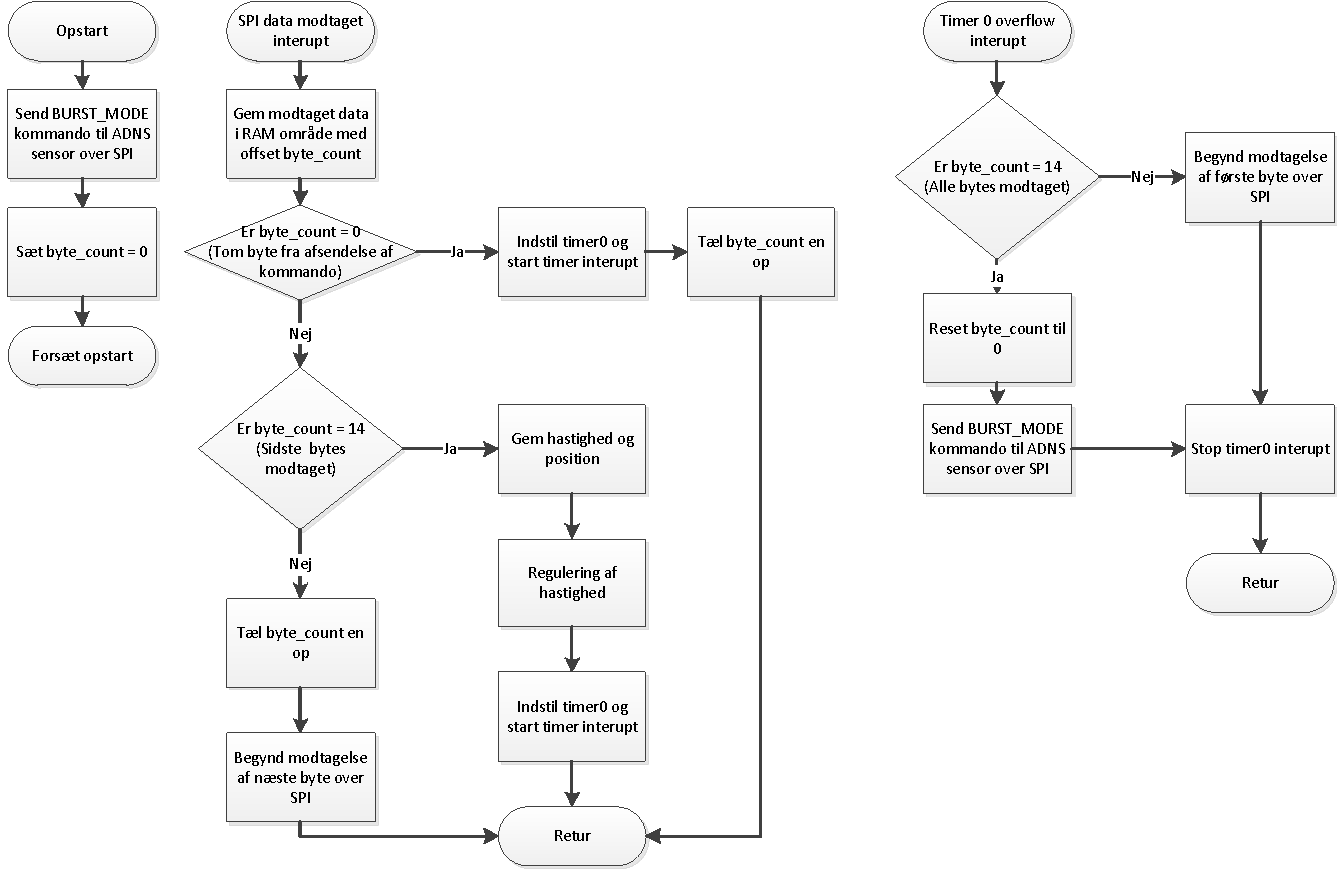
\includegraphics[scale=0.7]{ADNS_handling_met1.pdf}  
  \caption{Grafisk beskrivelse af hvordan afl�sningen af sensoren foreg�r}
  \label{fig:ADNS_handling_met1}
\end{figure}

\subsubsection*{Trin 1. Opstart af microcontroller}
Ved opstart af microcontrolleren indstilles SPI-enheden, t�ller v�rdien byte\_count s�ttes til 0 og den benyttede timer0 s�ttes op, s� den er klar til brug. Herefter sendes der en 0x00 (versionsnummer) kommando til sensoren, for at teste om kommunikationen er korrekt. Ved modtagelse af forkert svar, genstartes SPI-kommunikationen, og der springes tilbage til opstart af sensoren. N�r det korrekte svar (0x33) modtages, forts�ttes opstart ved at sende en r�kke kommandoer, der starter sensoren op. Deriblandt upload af firmware og kommandoer til at aktivere laseren og l�se \verb@MOTION@-byten p� sensoren. \verb@MOTION@ indeholder oplysninger om sensorens status, og kan blandt andet fort�lle, om laseren er korrekt startet op, eller om der er sket en fejl i sensoren. S�fremt der er fejl i laseren eller at der p� anden m�de meldes om fejl i \verb@MOTION@, fors�ges genstart af sensor, ellers sendes der en MOTION\_BURST kommando til sensoren, og microcontrollerens opstart forts�ttes.

\subsubsection*{Trin 2. Modtagelse af ''afsendelses''-byte}
N�r MOTION\_BURST kommandoen er sendt, kommer der et SPI overf�rselsinterrupt i microcontrolleren, fordi SPI-protokollen er asynkron og der derfor ogs� vil v�re modtaget data i samme tidsrum. I interruptet kontrolleres v�rdien byte\_count, og den vil i dette tilf�lde v�re lig med 0. Da sensoren har brug for $100$ $\mu s$ efter burstkommandoen er sendt, til at dataen i senoren er klar til afsendelse, s�ttes og aktiveres timeren timer0 samt timer0 overflow interrupt. Herefter afsluttes interruptet.

\subsubsection*{Trin 3. Klar til modtagelse af data}
Efter noget tid, vil timer0 udl�se et overflow interrupt, som f�lge af, at den afsatte tid til at klarg�re dataen i sensoren er g�et. I interruptet kontrolleres v�rdien af byte\_count, og den vil i dette tilf�lde v�re lige med 0, og derfor p�begyndes afsendelse af en tom byte for at modtage f�rste byte. Der t�lles en op i byte\_count, og interruptet afsluttes.

\subsubsection*{Trin 4. Modtagelse af byte}
SPI overf�rselsinterrupt aktiveres igen. Dataen gemmes i hukommelsen p� en foruddefineret adresse, hvor byte\_count l�gges til. Byte\_count �ges med en, s�ledes at den n�ste modtagede byte ikke bliver skrevet oven i samme adresse. Herefter afsluttes interruptet. Dette trin gentages ind til at byte\_count viser at alle 14 bytes er modtaget.

\subsubsection*{Trin 5. Alle bytes er modtaget}
N�r alle bytes er modtaget, bliver positions- og hastighedsv�rdierne i hukommelsen opdateret. Herefter p�begyndes hastighedsreguleringen der bliver beskrevet i sektion \ref{sec:hastighedsregulering}. For at opn� et passende tidsinterval mellem afhentning af data fra sensoren, startes nu timer0 og interruptet afsluttes.

\subsubsection*{Trin 6. P�begyndelse af n�ste datamodtagelse}
N�r timeren interrupter kontrolleres v�rdien af byte\_count. Hvis byte\_count t�lleren viser, at sidste byte er modtaget, s�ttes byte\_count lig med 0, og kommandoen for motion burst sendes igen til sensoren. Herefter p�begyndes trin 2 igen, og s�ledes forts�ttes l�sningen af dataen fra sensoren.

% Her kommer noget omkring timingen af afhenting af data
For at sikre at der er tid nok til at l�se data fra sensoren, er der udf�rt beregninger for at finde den totale tid, det tager at afvikle motion burst kommandoen.
SPI-bussen er nedskaleret med en faktor 8, s�dan at bussen k�rer med 2MHz. Det tager en clock p� SPI-bussen at overf�re 1 bit, og en SPI-clock tager $\sfrac{1}{(2\cdot10^{6})} = 500ns$. Derfor vil det tage $500ns \cdot 8 = 4000ns$ fra at der er sat data til afsendelse p� SPI bussen, til at dette er overf�rt. Yderligere timingtal der bliver brugt i denne beregning er m�lt ved brug af debuggeren i AVR Studio fra Atmel. Der er lavet en visualisering af, hvorn�r processoren er i brug p� figur \ref{fig:adns_timediag}, for at give en ide om, hvor meget det optager processoren, og hvad tiden g�r med.

%Clocken p� SPI bussen er skaleret ned med /8. Dvs. 16MHz/2 = 2MHz.
%1 Clock er derfor lig med (1/2000000)s = 500 nanoseconds
\begin{savenotes}
\begin{table}[htb]
	\begin{center}
	\begin{tabular}{l|l|l|r|r}
	
			Nr.\footnote{''Nr.'' refererer til numrene p� figur \ref{fig:adns_timediag}} 		& Opgave															& Processor opg	& Tid		& Pct.	\\
	\hline
			1							& Transmission af motion burst kommando									& Nej		&   4000 $ns$	& 1,87\%  \\
			1							& Modtagelse af tom byte og indstilling af timer				& Ja		&   3190 $ns$	& 1,49\%  \\
			2							& Sensor klarg�ring af data															& Nej		& 100000 $ns$	& 46,67\%	 \\
			3							& Afsendelse af 1. ''modtagelsesbyte''									& Ja		&   3190 $ns$	& 1,49\%	\\
			3							& Data transmission																			& Nej		&   4000 $ns$	& 1,87\%	\\
			3							& 13 gange afsendelse og data transmission							&	-			&	 93470 $ns$	& 43,62\%  \\
			3							& Modtagelse af sidste byte og start af timer						&	Ja		&   3440 $ns$	& 1,60\%  \\
			4 						& Sensor ventetid f�r ny motion burst (t$_{BEXIT}$)				& Nej		&    500 $ns$	&	0,23\%  \\
			4							& Afsendelse af ny motion burst kommando								& Ja		&   2500 $ns$	& 1,17\%  \\
	\hline
										&	Total tid benyttet																		&				& 214,29 $ \mu s $ &  \\
										& Beregningstid benyttet																&				&  53,79 $ \mu s$ & 25,10\%  \\
										& Transmission af data og sensor forsinkelser						&				&  160,5 $ \mu s$ & 74,90\%  \\
	\end{tabular}
	\end{center}
	\caption{Beregning af brugt tid ved afhentning af motion burst data}
	\label{tab:adns_timing} %%ref
\end{table}
\end{savenotes}

\begin{figure}[htb]
  \centering
  
\includegraphics[scale=0.08]{ADNS_timediag.pdf}  
  \caption{Visualisering af tidsforbrug ved burst mode. R�d = Beregning, Gr�n = Fri}
  \label{fig:adns_timediag}
\end{figure}

Som det ses i udregningen i tabel \ref{tab:adns_timing} tager det 214$\mu s$ at hente de 14 motion bytes fra sensoren. 
%Det er nu muligt at beregne, hvor mange motion bursts der kan hentes fra sensoren pr. sekund, og finde ud af om 
Ud fra at bilen bev�ger sig med op til $5$ $\sfrac{m}{s}$, og der �nskes en pr�cision p� $0,5$ $cm$, betyder dette, at dataen fra sensoren skal hentes 1000 gange pr. sekund. Det vil sige, at der skal bruges $1000 \cdot 214,29 \mu s = 0,21 s$ p� afhentning af data, s� dette vil ikke blive en begr�nsning. Ved 1000 hentninger pr. sekund skal processoren bruge $53,79\mu s \cdot 1000 = 53,79ms$ p� beregning over dette sekund. Det betyder at det vil optage 5,38\% af processorens regnekapacitet at h�ndtere afhentning af data fra sensoren.

%Afsendelse af byte										8*500ns   =   4000ns (Fritid)				 1,87%	
%interrupt															3,19us 		=   3190ns (Proc)					 1,49%
%Sensor klarg�ring af data							100us			= 100000ns (Fritid)				46,67%
%Afsendelse af 1. ''modtagelsesbyte''	3,19us		=   3190ns (Proc)					 1,49%
%
%
%			Data transmisson											8*500ns 	=   4000ns (Fritid)	 1,87%
%			interrupt ''indl�sning af modtaget byte og afsendelse af ny modtagelses byte''
%																						3,13us		=   3190ns (Proc)		 1,49%
%x13 (4000+3190)13 =																			 93470ns					43,62%
%
%Data transmission											8*500ns 	=   4000ns (Fritid)				 1,87%
%Modtagelse af sidste byte							3,44us		=   3440ns (Proc)					 1,60%			(Herunder ikke regnet hastighedregulering)
%
%tBEXIT																					=    500ns (Fritid)				 0,23%
%
%timer til afsendelse af ny motion burst	2,25us	= 	2500ns (Proc)					 1,17%
%
%FRITID: 				160 500 nanoseconds = 160.5 microseconds
%PROC:						53 790 nanoseconds = 53.79 microseconds
%TOTAL:					214 290 ns = 214,29 microseconds
%
%Den skal t�mmes 1000 gange / sek for at opn� 0.5 cm pr�cision.
%53 790 000 nanoseconds = 0.05379 seconds ~ 5%

\subsection{Hvordan virker SPI}
SPI st�r for Serial Peripheral Interface, og er en asynkron seriel protokol, der blandt andet benyttes til at tilslutte eksterne ADC, DAC og EEPROM enheder. SPI benytter sig af minimum 4 ledere, hvoraf to af dem bruges til selve dataoverf�rslen. %Der findes forskellige m�der at navngive disse 4 ledere p�. 
Herunder er navngivningen fra ADNS-9500 sensorens datablad benyttet til disse ledere: 
\begin{itemize}
	\item MOSI (Master Out Slave In)
	\item MISO (Master In Slave Out)
	\item SCLK (Shift Clock)
	\item NCS (Negeret Chip Select)
\end{itemize}
%\begin{table}[htb]
%	\begin{center}
%	\begin{tabular}{l|l}
%	MOSI (Master Out Slave In) 	& SDI \\
%	MISO (Master In Slave Out)	& SDO	\\
%	SCLK (Data Clock)			& SCLK (Shift Clock) \\
%	NCS (Negeret Chip Select)	& CE (Chip enable) \\
%	\end{tabular}
%	\caption{SPI}
%	\label{tab:spi}
%	\end{center}
%\end{table}

SPI-bussen er bygget s�dan op, at der er en hoved (''master'')-enhed p� bussen og en, eller flere, under (''slave'')-enheder. For hver slave-enhed der tilsluttes, skal der forbindes et dedikeret NCS ben mellem master og slave enheden. Dette er vist p� figur \ref{fig:spi_connectors}.

\begin{figure}[htb]
  \centering
  \includegraphics[scale=0.2]{spi_connectors.pdf}  
  \caption{Forbindelse mellem SPI master og en eller flere slave enheder}
  \label{fig:spi_connectors}
\end{figure}

N�r masterenheden skal udveksle data med en slave enhed p� bussen, s�ttes NCS benet, der er forbundet med slaven, til logisk lav, imens de andre enheders NCS ben s�ttes til h�j. N�r en slave-enhed f�r et 0 p� NCS benet, aktiveres kommunikationen med enheden. Masterenheden s�tter nu en clock p� SCLK benet, og for hvert puls sendes der data fra master til slave p� MOSI benet, og data fra slave til master p� MISO. N�r dataoverf�rslen er f�rdig stoppes clocken p� SCLK, og NCS benet til slaven s�ttes igen h�j.

Der findes 4 forskellige m�der at synkronisere clock pulsen med dataen, og de kan beskrives med CPOL (Clock Polaritet) og CPHA (Clock phase).

\begin{table}[htb]
	\begin{center}
	\begin{tabular}{l|l|l}
Mode		& CPOL	& CPHA \\
0		& 0		& 0 \\
1		& 0		& 1 \\
2		& 1		& 0 \\
3		& 1		& 1
	\end{tabular}
	\caption{SPI indstillinger}
	\label{tab:spi_settings}
	\end{center}
\end{table}

CPOL bestemmer polariteten af clock pulsen. I praksis betyder det om clock pulsen vendes p� hovedet, alts� om pulsen kommer fra h�j og g�r lav, eller om den kommer fra lav og g�r h�j. CPHA bestemmer om data er klar p� dataen er klar p� stigende eller faldende flanke. Figur \ref{fig:spi_bus_polarity_and_phase}\footnote{Billede taget fra \url{http://en.wikipedia.org/wiki/File:SPI_timing_diagram2.svg}} illustrerer dette.

\begin{figure}[htb]
  \centering
  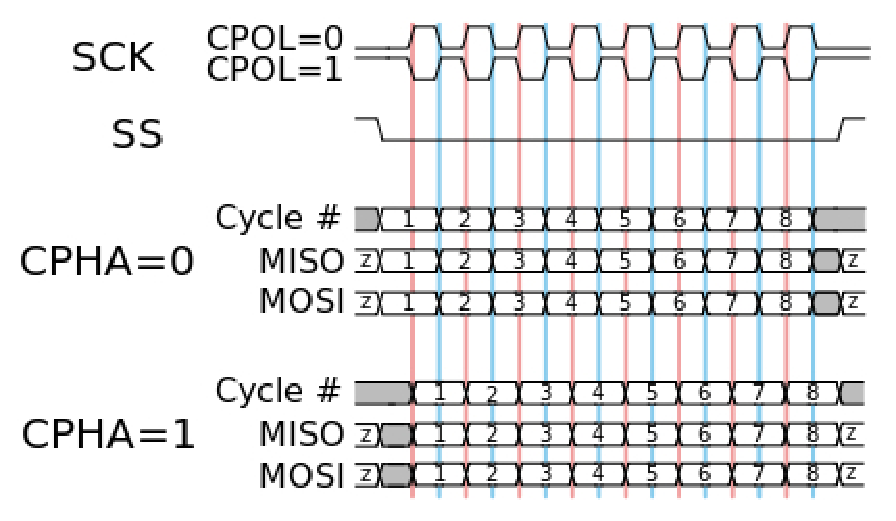
\includegraphics[scale=0.6]{spi_bus_polarity_and_phase.pdf}  
  \caption{Beskrivelse af CPOL og CPHA}
  \label{fig:spi_bus_polarity_and_phase}
\end{figure}

Derudover skal man v�re opm�rksom p�, hvorvidt det er det mest betydende (MSB) eller mindst betydende (LSB) bit, der sendes f�rst og frekvensen p� clocken mellem de to enheder skal k�re med.

Til kommunikation med ADNS-9500 sensoren benyttes mode 3 og MSB f�rst. Dette indstilles i ATmega32 microcontrollerens SPI registre. ATmega32 indeholder to registre, der skal indstilles, n�r man skal benytte sig at SPI interfacet. SPCR indeholder: SPI interrupt aktiveret, SPI aktiveret, Data Order (MSB eller LSB f�rst), Master select (Er ATmega32en master eller slave p� bussen), Clock Polaritet, Clock Fase, Clock hastighed

Derudover er der mulighed for at fordoble hastigheden p� SPI bussen i SPSR registeret, ved indstilling af bit 1.


\subsection{H-bro}\label{sec:hbro}
For at kunne benytte bilens motor, er der brug for at kunne styre str�mforsyninen til motoren. Microcontrollerens udgange er kun i stand til at levere f� milliampere, s� det er n�dvendigt at benytte en transistorl�sning til at kunne styre den forholdsvis store str�m, der skal drive motoren. I dette projekt er der benyttet en H-bro kobling af transistorne til styring af str�mmen gennem motoren. 
Ved at benytte en H-bro til styring af motoren, kan sp�ndingen over motoren skift retning, s�ledes at man b�de kan bruge motoren til en fremadrettet kraft og en bagudrettet kraft. Den bagudrettede kraft kan benyttes til at bremse bilen ned.

\begin{figure}[htb]
  \centering
  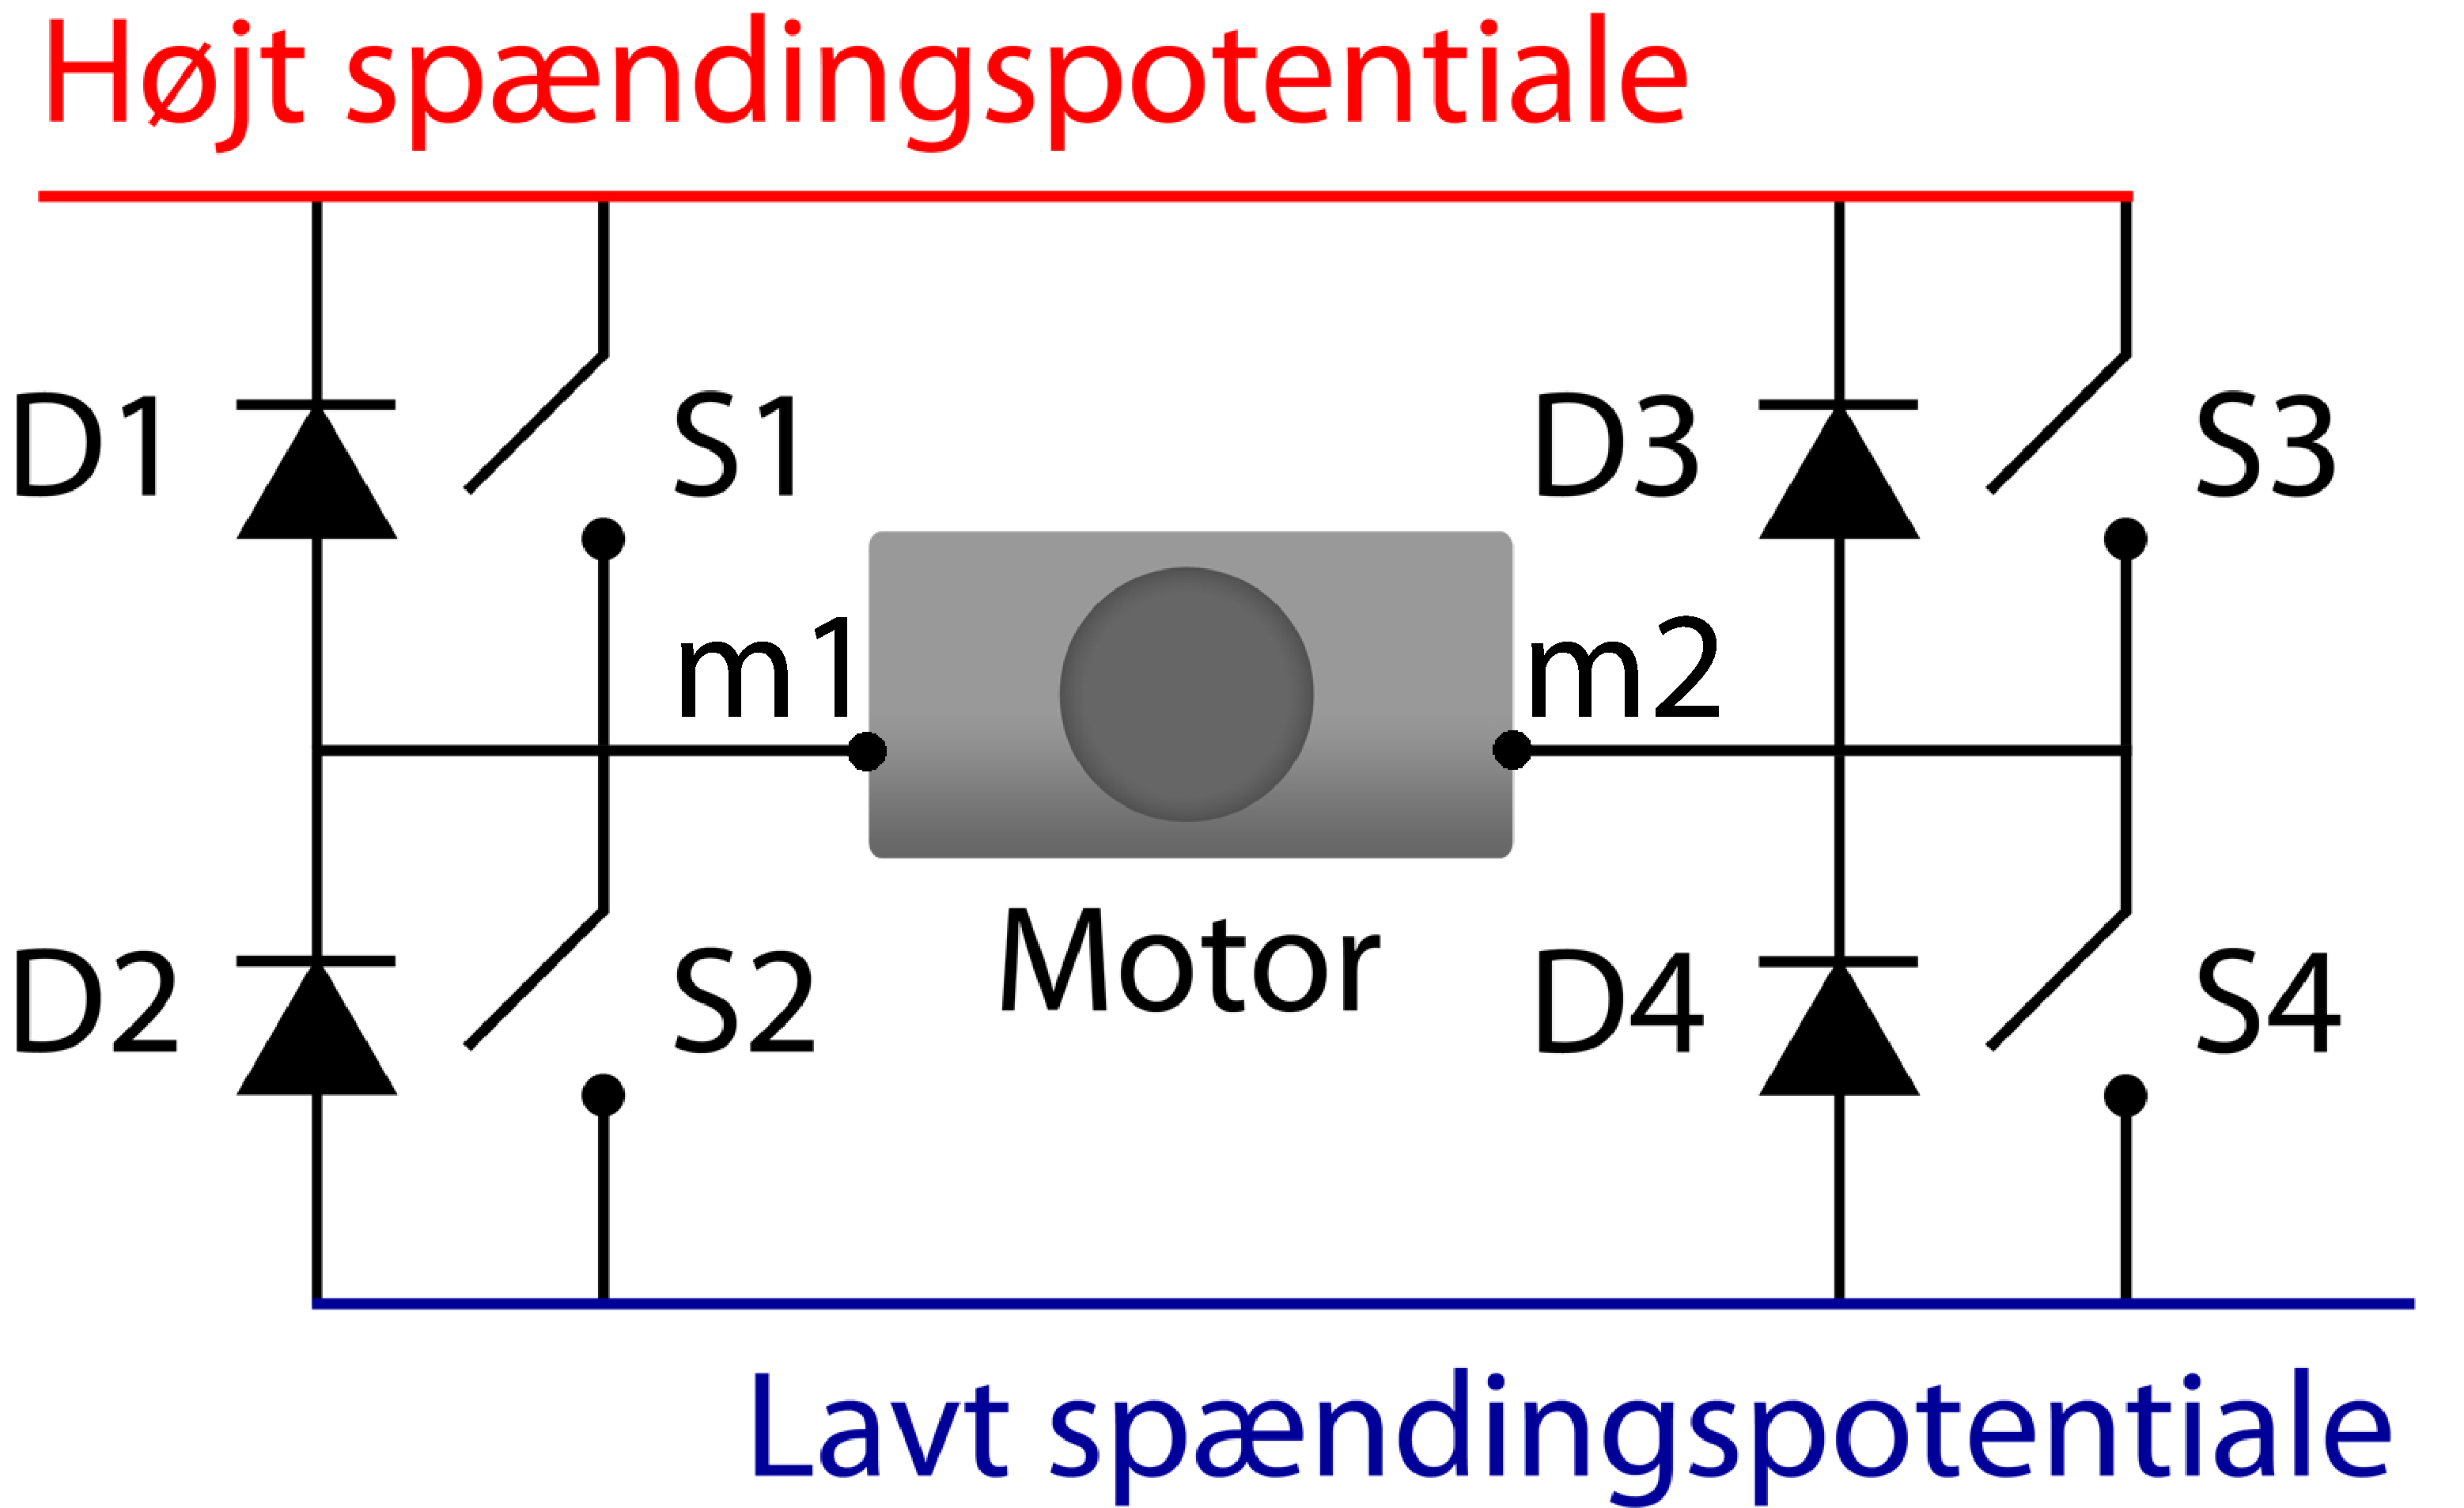
\includegraphics[scale=0.17]{hbro.pdf}  
  \caption{Forsimplet H-bro}
  \label{fig:hbro}
\end{figure}

H-broen kan betragtes som fire kontakter, der er fundet til motoren som vist p� figur \ref{fig:hbro}. Ved at slutte de viste kontakter i forskellige kombinationer, vil der kunne l�be en str�m gennem motoren afh�ngigt af dette. Hvis eks. S1 og S4 sluttes, mens S2 og S3 afbrydes, vil str�mmen l�be den ene vej. Sluttes i stedet for S2 og S3, mens S1 og S4 afbrydes, vil str�mmen l�be i modsat retning motoren. 
%En sidste mulighed er at man �bner for S2 og S4 samtidig, s�ledes begge ben p� motoren er forsynet med samme potentiale. Herved vil al den inducerede str�m i motoren kortsluttes, og dette vil give en

I praksis vil de beskrevede kontakter v�re udskiftet med transistorer, som s� er forbundet med microcontrolleren, s�dan at den har styringen med motoren.

P� figur \ref{fig:hbro} er der ligeledes beskrevet 4 dioder. Disse dioder er n�dvendige da motoren er forsynet med spoler, som inducerer en h�j sp�nding ved en pludselig �ndring af str�m gennem dem. I tilf�lde af en stor str�m fra motoren, vil denne have mulighed for at l�be gennem dioderne og undg� at �del�gge transistorne.

I opbygningen af bilen er der benyttet en f�rdig H-bro, som kommer i en integreret kreds. 

% Noget med IC kredsen


%I tabel \ref{tab:hbroconf} ses en liste over mulige indstillinger af disse ''kontakter''.

%\begin{table}[htb]
%	\begin{center}
%	\begin{tabular}{l|l|l}
%	
%	S1				& S2			& S3	& S4 & Indstilling		\\
%	\hline
%	Afbrudt		& Afbrudt	& Afbrudt 	& Afbrudt & Motor ikke forbundet til forsyning \\
%	Sluttet		& Afbrudt	& Afbrudt 	& Sluttet & Sp�nding over motoren, positiv retning \\
%	Sluttet		& Afbrudt	& Afbrudt 	& Sluttet & Sp�nding over motoren, negativ retning \\
%	ADNS-9500 				& 200ips 				& 30g				& Laser\\
%
%
%	\end{tabular}
%	\end{center}
%	\caption{Mulige indstillinger for H-broen}
%	\label{tab:hbroconf} %%ref
%\end{table}

%Noget med transistorer

%Noget med spolen og dioderne.






%En h-bro har den fordel, at man kan vende retningen af sp�ndingspotentialet over motoren, og i forbindelse med bilen, opn� en bremsende effekt. 

%En forsimplet H-bro best�r af 4 transistore, som vist p� figur \ref{fig:hbro}. 

%Grunden til at benytte en H-bro, er at man kan s�tte potentialet p� begge sider af motoren uafh�ngigt af hinanden. Det betyder at man kan s�tte begge ben til samme potentiale og opn� en bremsende effekt pga. 


%Der findes forskellige m�der at forbinde en transistor til motoren, s� det er muligt at styre den med en forholdsvis lille str�m, en af disse m�der kaldes for en H-bro. H



%h-bro

%Der er valgt en h-bor til bremse bil med. 
%opbygning og funktion
%	beskyttelses dioder
	
%kredsl�b

%m�llinger?


\newpage
\section{Programmering}
ATMega32 microcontrolleren, som Scalextric bilen er udstyret med, er samlingspunkt for al sensor input. Der f�s input fra musesensor, optocoupler, accelerometer og derudover skal motoren styres ud fra f�rn�vnte input. Alt dette er microcontrollerens opgave, hvilket alts� vil sige, at al aktivitet, der foreg�r, tager udgangspunkt i den software, der er skrevet til. I dette afsnit beskrives de forskellige programdeles form�l og funktion.

Den overordnede ide med softwaren er, at den skal v�re modul�r - forst�et p� den m�de, at det har skulle v�re let at �ndre bilens ''opf�rsel'' i forskellige situationer. Det har ledt til en opbygning af programmet, der er baseret p�, at der - enten manuelt eller ud fra sensorstimuli - kan skiftes mellem forskellige dele af programmet, ved at �ndre p� v�rdier i et register. �ndringen kan ske ligemeget hvor i programmet man befinder sig.

Den modul�re struktur af softwaren har lettet test af individuelle programstykker og har gjort, at den overordnede ide om k�rselsmetode har kunne f�lges. Der er s�ledes en del af softwaren, der tager sig af baneopm�ling og en der tager sig af k�rsel. Mellemliggende programniveauer s�tter rammen for hoveddelene. Enkelte dele, som f. eks. kommunikationsfunktionerne og ADNS sensordata opdatering, er konstant aktive.

\subsection{Programtilstande}
Som tidligere omtalt i sektion \ref{sec:metodevalg}, er det valgt, at der skal k�res ''opm�lt'' k�rsel. Det vil sige, at der f�rst k�res en eller, for den sags skyld, flere opm�lingsrunder, hvor det bestemmes til hvilke positioner bilen m�der sving. Derefter skal bilen skifte til at k�re efter de tidligere opm�lte data. Der er p� det grundlag blevet introduceret en r�kke forskellige \textit{tilstande}, som softwaren til bilen kan befinde sig i. Tilstand vil herfra blive brugt som en beskrivelse af, hvilken del af koden der eksekveres p� ATmega32 microcontrolleren.

En byte i hukommelsen bruges som statusregister: Afh�ngig af hvilke bits, der er sat, eksekveres bestemte stykker kode. Hvert stykke, eller tilstand, tjekker l�bende, om der er sket en �ndring af det n�vnte statusregister. Hvis der ikke er, forts�tter den ''i rundkreds''. Hvis der er, brydes der, og afh�ngig af hvad den nye tilstand er, k�res kode et nyt sted i programhukommelsen. Tabel \ref{tab:mode_bits} viser den byte, der indholder de flag, der bestemmer hvilken tilstand, der er aktiv.

\subsubsection*{MODE - Statusregister for tilstand}
\newcolumntype{K}{>{\centering\arraybackslash}X}%
\begin{table}[H]
	\begin{center}
	\begin{tabularx}{0.98\textwidth}{| K | c | c | K | K | K | K | K |}
	\multicolumn{1}{c}{7} & \multicolumn{1}{c}{6} & \multicolumn{1}{c}{5} & \multicolumn{1}{c}{4} & \multicolumn{1}{c}{3} & \multicolumn{1}{c}{2} & \multicolumn{1}{c}{1} & \multicolumn{1}{c}{0} \\
	\hline
	\verb@MD_SET@ & \verb@-@ & \verb@-@ & \verb@MD_PRERACE@ & \verb@MD_PREWARM@ & \verb@MD_RACE@ & \verb@MD_WARM@ & \verb@MD_DEF@ \\
	\hline
	\end{tabularx}
	\end{center}
	\caption{MODE register}
	\label{tab:mode_bits} %%ref
\end{table}

\begin{itemize}
	\item \textbf{Bit 7 - Settings Flag}\\
	Dette flag er det eneste, der er f�lles for de forskellige tilstande. I det en ny tilstand aktiveres bliver dette flag nulstillet. Dermed ved den nye tilstand, at den skal s�tte indstillinger for netop den nye tilstand. Hver tilstand har et antal forskellige ting, der skal initialiseres f�r hovedrutinen udf�res. S� snart det er sket, s�ttes \verb@MD_SET@, og det bliver ved med at v�re sat, indtil der skiftes til en ny tilstand.
	\item \textbf{Bit 6:5 - Reserveret}\\
	Disse bits er ikke brugt og bliver ikke l�st, men de er reserveret til eventuelt senere brug. Der b�r derfor skrives 0 til dem i alle tilf�lde.
	\item \textbf{Bit 4 - Pre-race tilstand}\\
	Dette bit er 1 n�r pre-race tilstand er sat. Pre-race tilstand er trinnet f�r race tilstand, og det tidspunkt i koden, hvor beregninger foretages som forberedelse til den egentlige tidsk�rsel.
	\item \textbf{Bit 3 - Pre-warmup tilstand}\\
	Dette bit er 1 n�r pre-warmup tilstand er sat. I pre-warmup tilstand s�ges der efter m�lstregen s�ledes, at warmup tilstanden kan aktiveres, s� snart m�llinjen krydses.
	\item \textbf{Bit 2 - Race tilstand}\\
	Dette bit er 1 n�r race tilstand er sat. Dette er tidsk�rslen, hvor den hurtigst mulige omgangstid �nskes sat. Data indsamlet i warmup tilstand benyttes til at bestemme hvordan og hvorn�r hastigheden skal �ndres.
	\item \textbf{Bit 1 - Warmup tilstand}\\
	Dette bit er 1 n�r warmup tilstand er sat. Warmup tilstand er den programrutine, hvor der indsamles data: Hvorn�r der forekommer sving, og til hvilken position det sker.
	\item \textbf{Bit 0 - Default tilstand}\\
	Dette bit er 1 n�r default tilstand er sat. N�r default tilstand er aktiv, foretager bilen sig intet af sig selv. Alle funktioner er passive og f. eks. k�rsel, eller start af automode, sker kun ved input fra brugeren.
\end{itemize}
Kun et af de tilstandsbestemmende bits b�r v�re sat ad gangen.

\begin{figure}[htb]
	\begin{center}
	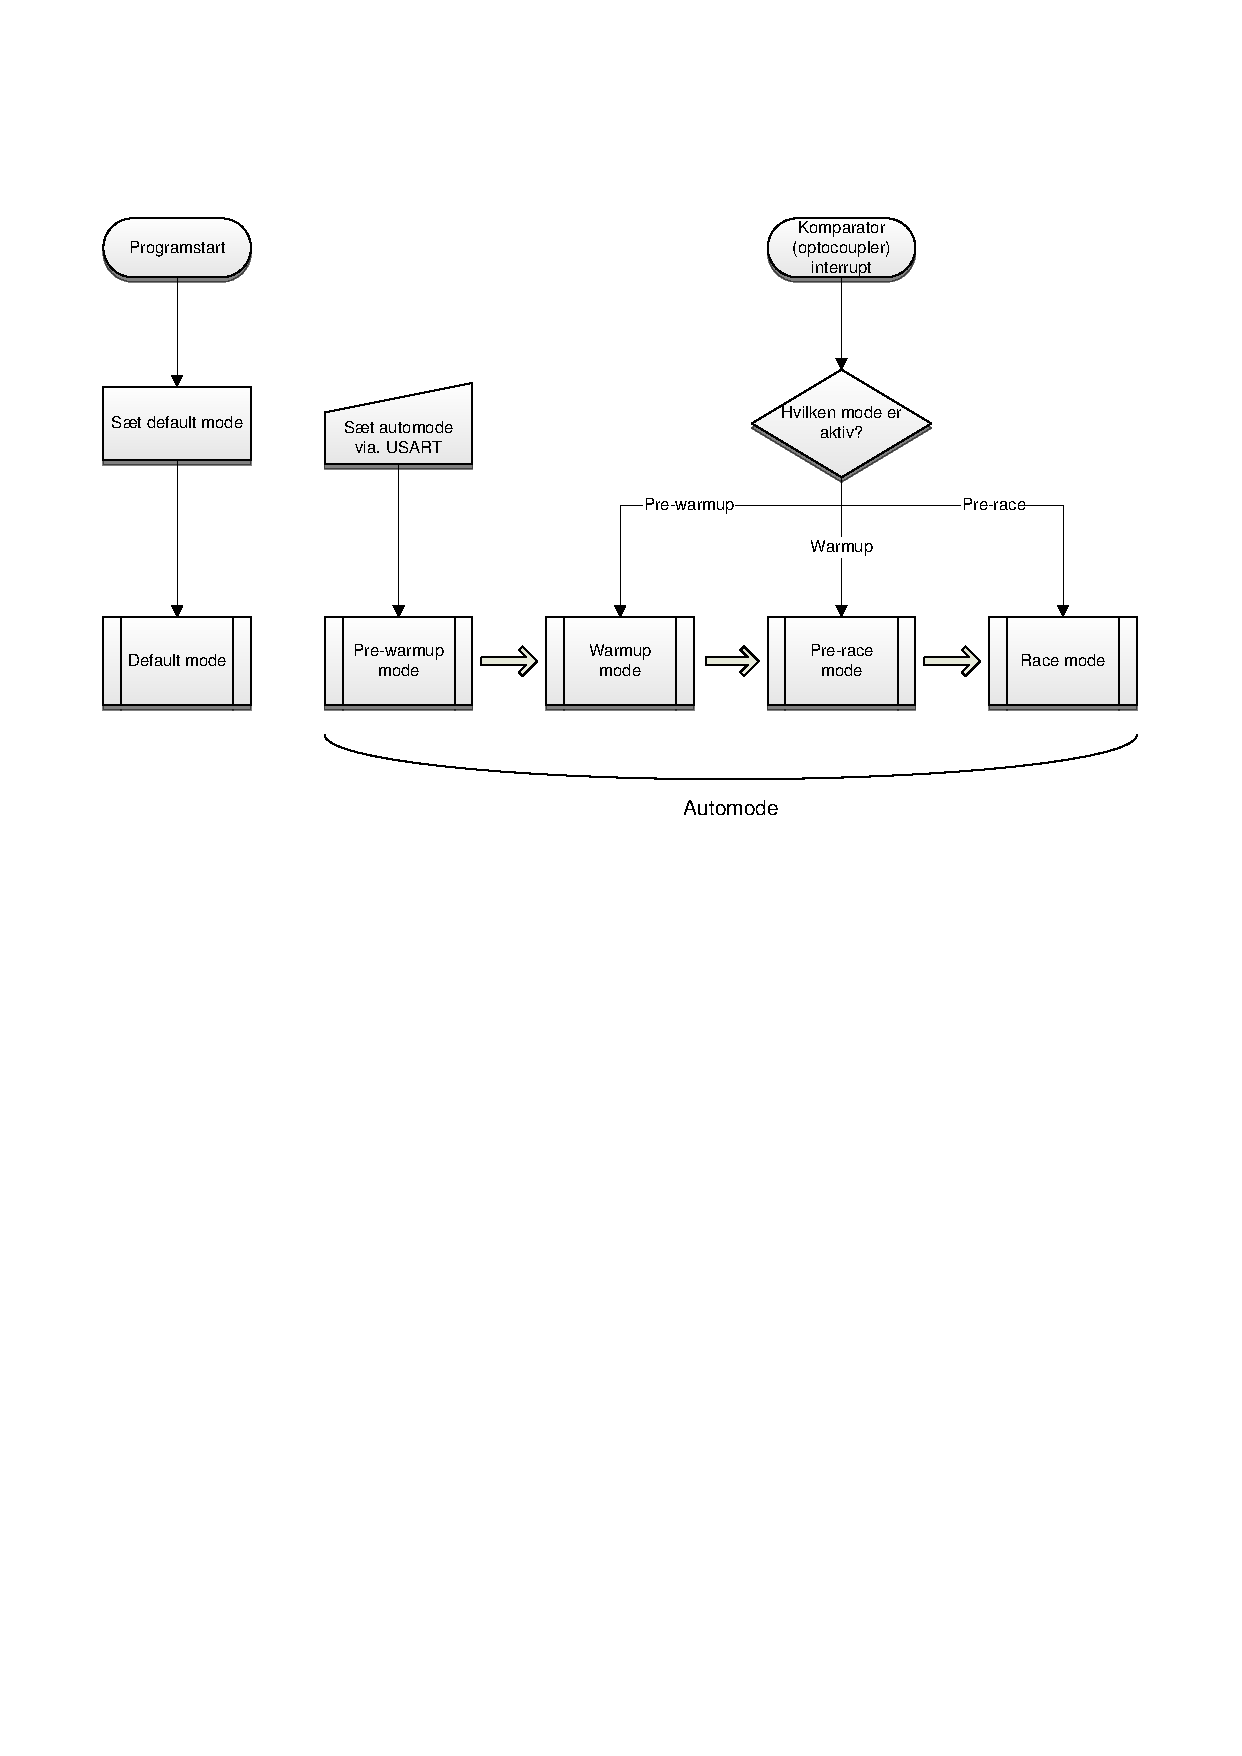
\includegraphics[page=1,scale=0.80,trim=30 440 0 100]{modes.pdf} %trim=l b r t
	\caption{Programtilstande}
	\label{fig:modes}
	\end{center}
\end{figure}

Det er et krav til projektet, at bilen skal kunne startes med \textit{automode}-kommandoen og derefter k�re autonomt. Figur \ref{fig:modes} illustrerer, hvordan automode best�r af pre-warmup, warmup, pre-race og race-tilstand. Ved boot s�ttes default tilstand som udgangspunkt. Der skal s� et manuelt input (GET-telegram via. USART) til at aktivere automode, som her begynder i pre-warmup tilstand.

N�r pre-warmup tilstand er sat, kan bilen klare sig p� egen h�nd. N�r m�lstregen krydses, s�rger komparator interruptrutinen (udl�st n�r optocoupleren passerer m�lstregen) for at skifte til n�ste tilstand i r�kkef�lgen: Pre-warmup, warmup, pre-race og race. Komparatorinterruptet aktiverer timer1 overflow interruptet for at tilf�je en forsinkelse, f�r komparatorinterruptet n�ste gang kan udl�ses. Grunden til dette er, at at m�lstregen ellers kan udl�se flere komparatorinterrupts, hvis ikke den er fuldst�ndig j�vn.

Pre-warmup og pre-race tilstandene er, som n�vnt, forl�bere til warmup og race tilstandende, henholdsvis. Derfor beskrives efterf�lgende warmup-og racetilstand i detaljer.

\subsubsection{Warmup}
Warmup-tilstand er, hvor banen m�les op ved en hastighed, hvor det er sikkert, at bilen ikke falder af. M�let er at detektere, hvorn�r bilen k�rer ind i et sving, og hvorn�r den k�rer ud af det. Det vil sige, at analog-til-digital konverteren, og dermed accelerometerv�rdien, skal afl�ses l�bende, og n�r et udslag detekteres, skal positionen, hvor det sker, gemmes. Til det form�l oprettes en tabel i SRAM, herfra kaldet \verb@EVTTBL@, som indeholder position samt om der drejes (og hvilken retning), eller om der k�res ligeud. Det er vigtigt at notere, at det kun er, n�r der sker en \textit{�ndring} fra sving til et lige stykke, eller omvendt, at der skal gemmes et datas�t. \verb@EVTTBL@ ser ud som vist i Tabel \ref{tab:evttbl}, hvor \verb@Pos[5:0]@ er de 6 bytes, der gemmer nuv�rende position (opdateret l�bende af SPI interruptrutinen, der l�ser data fra ADNS9500 sensoren). \verb@TURNSTS@ er en v�rdi, bestemt af en ADC m�ling, der fort�ller om h�ndelsen beskrevet er et h�jre- eller venstresving eller et lige banestykke. \verb@TURNSTS@ kan antage v�rdierne 0x01 (lige ud), 0x02 (venstre) og 0x04 (h�jre). \verb@Pos[x]@$_{y}$ betegner en m�lt v�rdi.

\begin{table}[htb]
	\begin{center}
	\begin{tabular}{c|c|c|c|c|c|l}
	\multicolumn{6}{c|}{Position} & \verb@TURNSTS@\\
	\hline
	\verb@Pos[5]@$_{0}$ & \verb@Pos[4]@$_{0}$ & \verb@Pos[3]@$_{0}$ & \verb@Pos[2]@$_{0}$ & \verb@Pos[1]@$_{0}$ & \verb@Pos[0]@$_{0}$ & \verb@TURNSTS@$_{0}$ \\
	\hline
	\verb@Pos[5]@$_{1}$ & \verb@Pos[4]@$_{1}$ & \verb@Pos[3]@$_{1}$ & \verb@Pos[2]@$_{1}$ & \verb@Pos[1]@$_{1}$ & \verb@Pos[0]@$_{1}$ & \verb@TURNSTS@$_{1}$ \\
	\hline
	\verb@Pos[5]@$_{2}$ & \verb@Pos[4]@$_{2}$ & \verb@Pos[3]@$_{2}$ & \verb@Pos[2]@$_{2}$ & \verb@Pos[1]@$_{2}$ & \verb@Pos[0]@$_{2}$ & \verb@TURNSTS@$_{2}$ \\
	\hline
		... & ... & ... & ... & ... & ... & \multicolumn{1}{|c}{...}
	\end{tabular}
	\end{center}
	\caption{EVTTBL}
	\label{tab:evttbl} %%ref
\end{table}

I l�bet af pr�vek�rsler opdagedes der, at de m�linger, der optages af analog-til-digital konverteren, ind imellem kan \textit{spike} (se Appendiks \ref{sec:bilag_acc}). Det vil sige, at der er risiko for, at der detekteres sving, hvor der i virkeligheden ikke er det. Det har alts� ikke v�ret nok bare at holde �je med udslag fra accelerometeret. Det har p� det grundlag v�ret n�dvendigt at modificere koden, der l�ser ADC v�rdier, til ikke uden videre at ''godkende'' og gemme alle m�linger. N�r warmup-tilstand er aktiv, genneml�bes koden, der herunder beskrives, helt indtil der skiftes tilstand igen, efter der er k�rt en omgang p� banen, og m�lstregen krydses.

\begin{figure}[htb]
	\begin{center}
	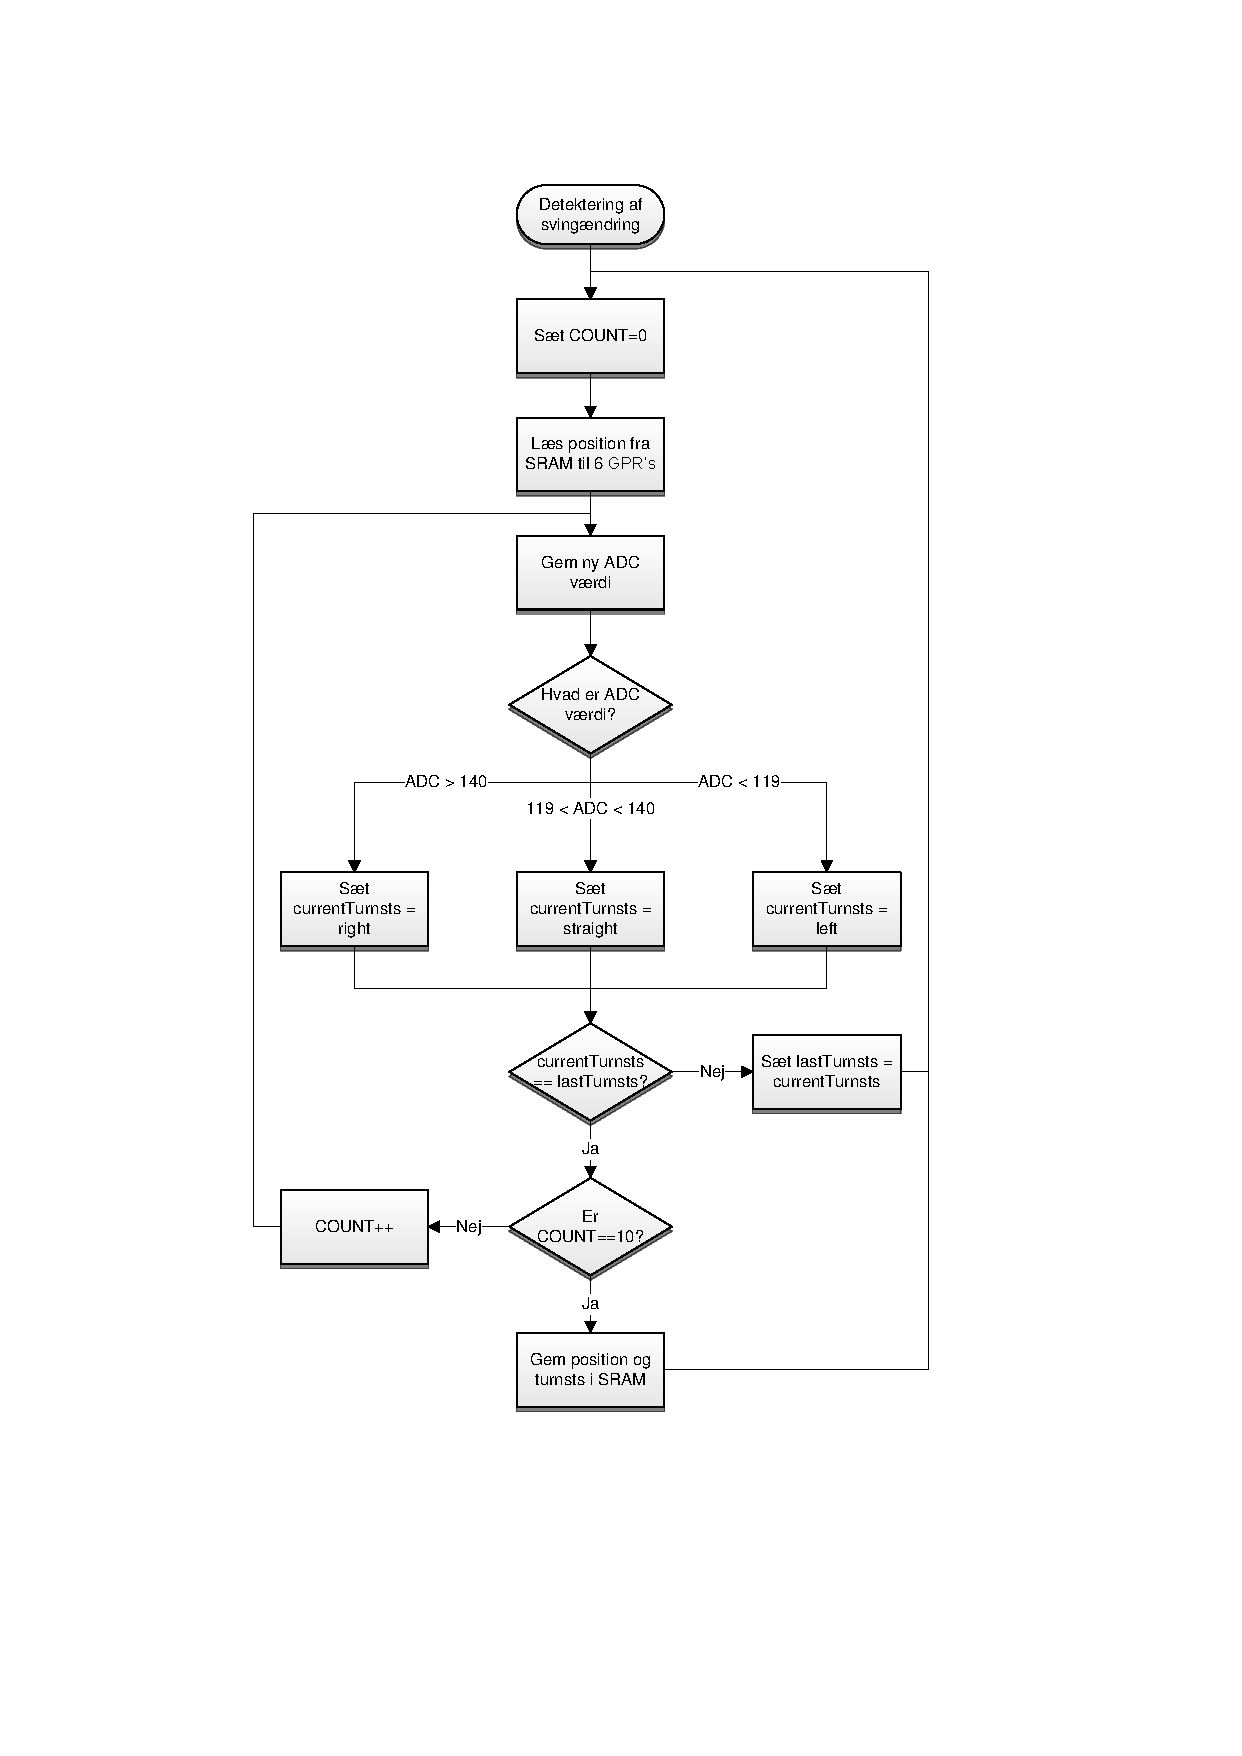
\includegraphics[page=1,scale=0.80,trim=150 162 150 108]{adc_logging.pdf} %trim=l b r t
	\caption{Detektering af sving�ndring}
	\label{fig:acd_log}
	\end{center}
\end{figure}

S� snart warmup tilstand aktiveres initialiseres en pointer\footnote{16-bit v�rdi - gemt i to 8-bit registre - der peger p� en adresse i SRAM} til at pege p� \verb@EVTTVL@ hvorefter en ADC konvertering startes. S� snart den f�rste konvertering er begyndt forl�ber processen som vist p� Figur \ref{fig:acd_log}. Ideen bag l�kken er, at der skal 10 ADC (og dermed accelerometer) m�linger til for at et ny �ndring af sving logges. Alle 10 m�linger skal konvergere enten over 140 (h�jresving), under 119 (venstresving) eller mellem de to v�rdier (lige ud). Hvis ikke de g�r det, begyndes en ny m�leserie. Positionen til stedet hvor en sving�ndring sker, l�ses altid \textit{f�rste} gang en �ndring detekteres, s� der ikke forekommer en forskydelse fra den egentlige sving-position, til den m�lte. T�rkselv�rdierne for, hvorn�r sving registreres, er bestemt ud fra m�linger af accelerometerdata - se Appendiks \ref{sec:bilag_acc}.

For hver sving�ndring, der gemmes i hukommelsen, �ges pointerv�rdien med 7 (6 byte til position og 1 til \verb@TURNSTS@ v�rdien). N�r warmup-tilstand ender (n�r m�lstregen krydses og pre-race tilstand aktiveres) s�ttes bilens position til 0 og pointerv�rdien gemmes p� en fast adresse i SRAM, s� b�de start- og slutadressen p� \verb@EVTTBL@ er kendt.
%
%		PSEUDO/C-KODE til ADC sving detektering
%
%\begin{lstlisting}[language=C,caption={pseudo},label={code:temp}]
%
%//Der skal bruges 10 m�linger i tr�k, hvor der drejer samme vej for at en sving�ndring logges
%while (c < 10)
%{
%	//L�s nuv�rende ADC v�rdi
%	adcVal = ADCH;
%	
%	//Bestem om der k�res til h�jre, venstre eller ligeud
%	if (adcVal > thresholdHigh)
%	{
%		currentTurnsts = right;
%	}
%	else if (adcVal < thresholdLow)
%	{
%		currentTurnsts = left;
%	}
%	else
%	{
%		currentTurnsts = straight;
%	}
%	
%	//Hvis vi drejer samme vej som forrige check �ges counteren, hvis ikke resettes den
%	if (currentTurnsts == lastTurnsts)
%	{
%		c++;
%	}
%	else
%	{
%		c = 0;
%	}
%	
%	//Der "huskes" hvilken retning der lige er blevet k�rt i
%	lastTurnsts = currentTurnsts;
%}
%
%//Idet counteren n�r 10 gemmes position og sving-retning
%saveValues();
%
%\end{lstlisting}
%

\subsubsection{Race}
N�r race-tilstand aktiveres begynder k�rsel efter en ny tabel i hukommelsen: \verb@DRVTBL@. Det er en tabel, der oprettes i l�bet af pre-race tilstand. Den indeholder position og en beregnet hastighed, hvormed bilen skal k�re. Hastigheden er den eneste variabel der kan �ndres under k�rsel - det s�rger hastighedsreguleringen\footnote{Se sektion \ref{sec:hastighedsregulering} om hastighedsregulering} for. Der omregnes fra en sving-betegnelse (\verb@TURNSTS@) til en hastighed f�r den egentlige tidsk�rsel indtr�der for at mindske kravet til ledige clockcycles i microcontrolleren. Hvis \verb@TURNSTS@ f�rst skulle l�ses, og derefter bruges til at bestemme en hastighed, ville det optage un�dig processortid under tidsk�rslen. Der er til geng�ld nok plads i SRAM til at lagre \verb@DRVTBL@ uden konsekvenser.

Omregningen fungerer ved, at der indl�ses et datas�t, alts� en tabelr�kke p� 7 bytes, fra \verb@EVTTBL@ i SRAM til registre $r0$ $<$ $R$ $<$ $r31$, s� der kan arbejdes med dataen. Form�let er at l�se en position, hvortil der vides, om bilen enten er p� vej \textit{ind} i et sving eller p� vej \textit{ud} af det. Det fort�ller \verb@TURNSTS@-v�rdierne forskellige steder p� banen. De tre forskellige scenarier, der kan bestemmes ud fra de m�lte data i warmup-tilstand er vist i Tabel \ref{tab:turnstsvals}.

\begin{table}[htb]
	\begin{center}
	\begin{tabular}{l|l}
	 \multicolumn{1}{c|}{K�resituation} & \verb@TURNSTS@ \\
	\hline
	 Fra et lige banestykke til et h�jresving & 0x04\\
	 Fra et lige banestykke til et venstresving & 0x02\\
	 Fra et sving til et lige stykke & 0x01\\
	\end{tabular}
	\end{center}
	\caption{TURNSTS-v�rdier i forskellige k�resituationer}
	\label{tab:turnstsvals} %%ref
\end{table}

Figur \ref{fig:banemapping} viser et banestykke med et sving. Scalextricbilen k�rer fremad og er p� vej ind i svinget ved punkt $A$. Lidt senere k�rer den ud af svinget ved punkt $B$. Punkt $A$ og $B$ m�ltes i l�bet af warmup-tilstand og har dermed f�et \verb@TURNSTS@-v�rdierne: \verb@TURNSTS@$_{A}$ = 0x04 og \verb@TURNSTS@$_{B}$ = 0x01 med tilh�rende position \verb@Pos[5:0]@$_{A}$ og \verb@Pos[5:0]@$_{B}$. Der �nskes at bestemme en ny position, \verb@Pos[5:0]@$_{A}'$, som er den, hvor hastigheds�ndringen (her s�nkelse af hastigheden f�r sving $A$) skal ske. Den nye position bestemmes ved at tr�kke en konstant fra \verb@Pos[5:0]@$_{A}$, s�ledes at hastighedsjusteringen kan ske \textit{f�r} svinget n�s. Bilen har nemlig en vis bremsel�ngde\footnote{Se appendiks \ref{sec:bilag_hbrotest} om test med H-bro}, som der skal tages h�jde for. N�r bilen k�rer ud af svinget, kan hastigheden ogs� godt justeres op, f�r den er helt ude p� det lige stykke.

\begin{figure}[htb]
	\begin{center}
	\includegraphics[page=1,scale=0.24,trim=0 0 0 0]{banemapping.pdf} %trim=l b r t
	\caption{Mapping af banestykke}
	\label{fig:banemapping}
	\end{center}
\end{figure}

Ligesom der findes tre forskellige v�rdier for \verb@TURNSTS@ findes tre forskellige v�rdier for offset konstantenterne, herfra kaldet \verb@OS@$_{TURNSTS_{RIGHT}}$, \verb@OS@$_{TURNSTS_{LEFT}}$ og \verb@OS@$_{TURNSTS_{STRAIGHT}}$ (ogs� vist p� Figur \ref{fig:banemapping}). De er bestemt ved pr�vek�rsel p� en test bane. P� samme grundlag findes der 3 forskellige hastigheder, \verb@V@$_{RIGHT}$, \verb@V@$_{LEFT}$ og \verb@V@$_{STRAIGHT}$, som liges� er bestemt empirisk. Hastighederne er 8-byte v�rdier og maksimal opl�sning er, som f�lge af det, 256.

Den nye tabel, \verb@DRVTBL@, som der skal f�lges under tidsk�rsel f�r p� den m�de samme struktur som \verb@EVTTBL@, men med en hastighedsv�rdi, \verb@V@, som erstatning for for \verb@TURNSTS@, og en ny position, \verb@Pos[5:0]@$_{}'$.

\begin{table}[htb]
	\begin{center}
	\begin{tabular}{c|l c c|l}
	\multicolumn{2}{c}{EVTTBL} & & \multicolumn{2}{c}{DRVTBL} \\
	\cline{1-2} \cline{4-5}
	Position & \verb@TURNSTS@ & & Position' & \verb@V@ \\
	\cline{1-2} \cline{4-5}
	\verb@Pos[5:0]@$_{0}$ & \verb@TURNSTS@$_{0}$ & 								& 
	\verb@Pos[5:0]@$_{0}'=$ \verb@Pos[5:0]@$_{0}-$\verb@OS@$_{TURNSTS_{0}}$ & \verb@V@$_{0}$ \\
	
	\verb@Pos[5:0]@$_{1}$ & \verb@TURNSTS@$_{1}$ & $\Rightarrow$ 	& 
	\verb@Pos[5:0]@$_{1}'=$ \verb@Pos[5:0]@$_{1}-$\verb@OS@$_{TURNSTS_{1}}$ & \verb@V@$_{1}$ \\
	
	\verb@Pos[5:0]@$_{2}$ & \verb@TURNSTS@$_{2}$ & 								& 
	\verb@Pos[5:0]@$_{2}'=$ \verb@Pos[5:0]@$_{2}-$\verb@OS@$_{TURNSTS_{2}}$ & \verb@V@$_{2}$ \\
	
	... & \multicolumn{1}{c}{...} & & ... & ...
	\end{tabular}
	\end{center}
	\caption{Omregning fra EVTTBL til DRVTBL}
	\label{tab:drvtbl} %%ref
\end{table}

Selve k�rslen foreg�r ved l�bende at l�se en tabelr�kke fra \verb@DRVTBL@-tabellen og sammenligne bilens position til et bestemt �jeblik med den, der st�r i tabellen. S� snart bilens position er den samme, eller over den, der st�r i \verb@DRVTBL@, skal en eventuel hastigheds�ndring udf�res og en ny tabelr�kke indl�ses. K�rer bilen over m�lstregen nulstilles dens nuv�rende positionsv�rdi. P� samme tidspunkt skulle enden af \verb@DRVTBL@ v�re n�et, og der startes igen fra begyndelsen af tabellen.
\subsection{Hastighedsregulering}
\label{sec:hastighedsregulering}

Som en del af strategien med at k�re en runde for at finde alle svingene og herefter beregne maksimal hastigheden, er der lavet en regulering, som st�r for at justere signalet til motoren, s�ledes at bilens hastighed er s� t�t p� den �nskede hastighed som muligt. Alternativt kan man antage, at bilen har en bestemt hastighed ved et givet motorsignal, men fordi bilens hastighed afh�nger af langt flere faktorer end dette, er denne l�sning ikke acceptabel til dette form�l. Hastighedsreguleringen vil blandt andet elliminere problemer med sp�ndingsfaldet i banens indflydelse p� motorhastigheden, da motorenshastighed er afh�ngig af dens forsyning fra banen. Form�let er derudover ogs� at optimere nedbremsningen i svingene og, hvis n�dvendigt, at vende sp�ndingen over motoren ved hj�lp af h-broen (se appendix \ref{sec:bilag_hbrotest}) med henblik p� at levere en stor modsat rettet accelleration og derved effektivt bremse bilen til den �nskede hastighed.

Styring af bilens motor foreg�r ved hj�lp at et puls-bredde-moduleret signal, ogs� kaldet PWM "Pulse Width Modulation". Et PWM signal har kun to tilstande, logisk h�j (t�ndt) eller logisk lav (slukket). Udtrykket "Duty cycle" beskriver, hvor stor en del af en periode, signalet befinder sig i h�j tilstand. Afh�ngigt af H-broens tilstand, vil det betyde at des h�jere duty cyclen bliver, des mere energi tilf�res der til motoren. Et eksempel p� et PWM signal er vist p� figur \ref{fig:pwm}.

\begin{figure}[htb]
  \centering
  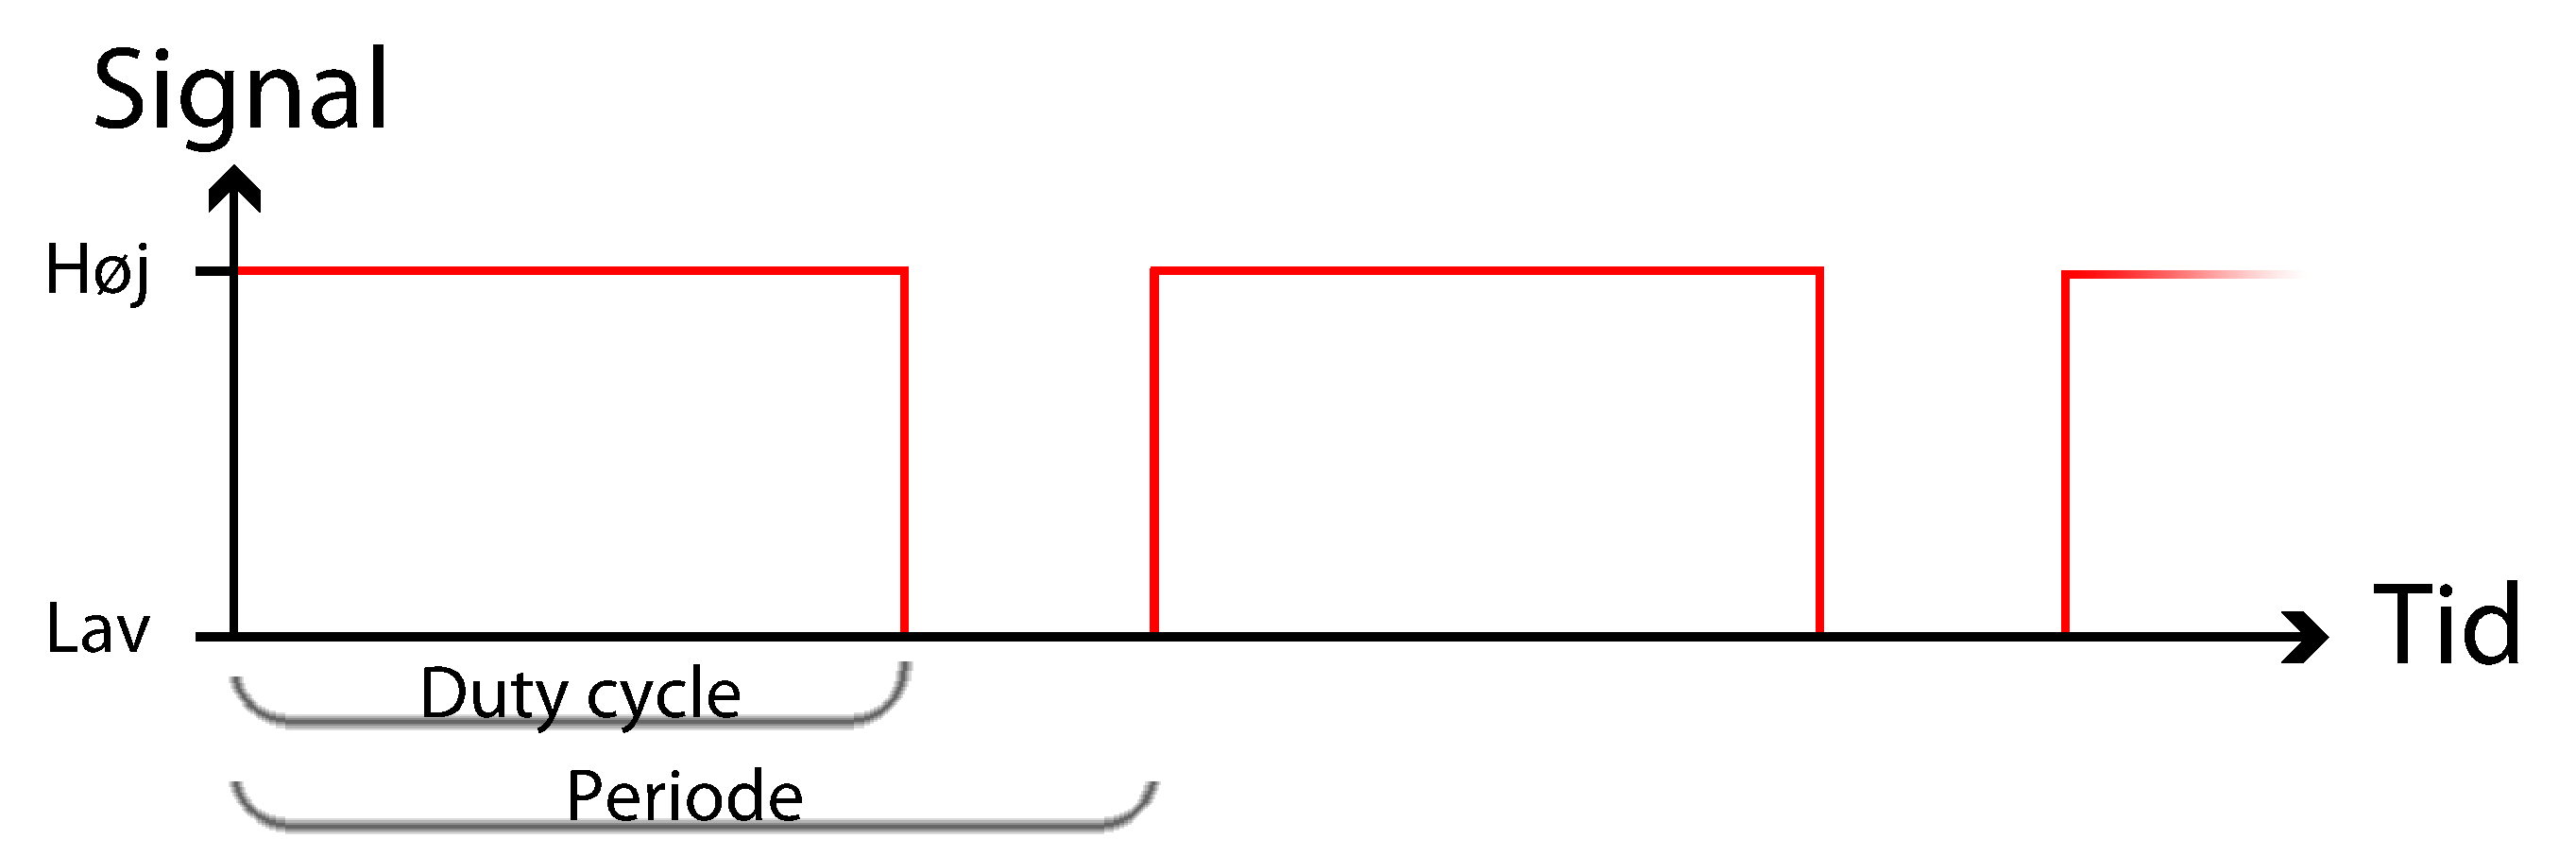
\includegraphics[scale=0.27]{pwm.pdf}  
  \caption{Beskrivelse af PWM}
  \label{fig:pwm}
\end{figure}


Ved brug af et PWM signal holder man transistorne i h-broen udenfor det aktive omr�de st�rstedelen af tiden ved enten at lukke helt op for transistoren eller lukke helt i. Dette afs�tter en langt mindre effekt i transistoren, da den kun befinder sig i det aktive omr�de, og dermed kun afs�tter effekt, i det �jeblik der skiftes mellem �ben og lukket tilstand p� transistoren i h-broen. PWM signalet kan genereres direkte p� en af microcontrolerens timere, ved hj�lp af compare v�rdien.

Hastighedsreguleringen p� bilen er en simpel line�r regulering. Det vil sige, at des mere den nuv�rende hastighed afviger fra den �nskede, des st�rre �ndring tilf�res motorens PWM. Program koden til hastighedsreguleringen virker som vist p� figur \ref{fig:ADNS_speedcalculation_1}. Yderligere forklaring f�lger efter figuren.

Til regulering af bilens hastighed, er der benyttet en simpel model, hvor der benyttes en feedback i form af bilens hastighed til at justere imod den �nskede hastighed. Dette er illustreret p� figur \ref{fig:hastighedsregulering}.

\begin{figure}[htb]
  \centering
  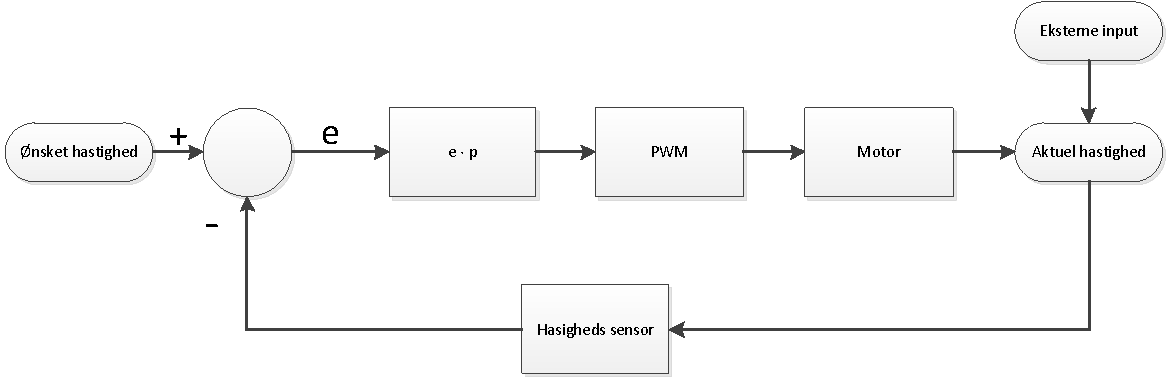
\includegraphics[scale=0.75]{Hastighedsregulering.pdf}  
  \caption{Reguleringssl�jfe}
  \label{fig:hastighedsregulering}
\end{figure}

Hastighedsreguleringen virker ved, at den har f�et angivet en �nsket hastighed fra den �vrige programkode i bilen. Den aktulle hastighed afl�ses ved hj�lp af musesensoren, og tr�kkes fra den �nskede hastighed, s�ledes at resultatet heraf repr�senterer afvigelsen fra den aktuelle hastighed og dermed fejlen. Fejlen multipliceres med en konstant og adderes til PWM-signalet. S�ledes er fejlen proportional med �ndringen af duty cyclen p� PWM-signalet. S�ledes vil en stor fejl betyde en stor �ndring i PWM-signalet for at mindske denne fejl. Konstanten kan tilpasses efter at opn� optimal regulering, s� den er tilstr�kkelig stor til at fejl korrigeres hurtigt uden at reguleringen g�r i selvsving. Selvsving kan opst�, hvis konstanten bliver for stor, og en lille fejl herved multipliceres til en alt for stor korrektion, s�ledes at fejlen bliver st�rre i modsat retning.

\begin{figure}[H]
  \centering
  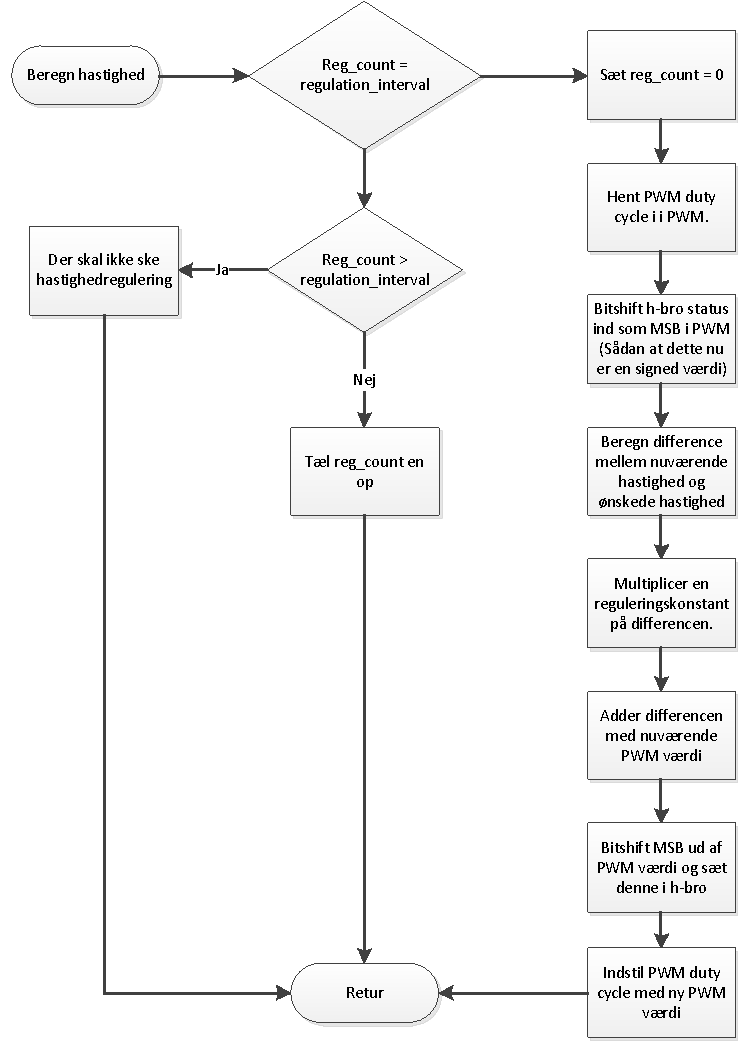
\includegraphics[scale=0.75]{ADNS_speedcalculation_1.pdf}  
  \caption{Programbeskrivelse af hastighedsregulering}
  \label{fig:ADNS_speedcalculation_1}
\end{figure}

I programkoden sker reguleringen ved, at H-broens retning bliver bit-shiftet ind og sat som fortegn p� nuv�rende PWM-v�rdi. Det betyder, at PWM-v�rdien nu er en signed byte, der angiver retning og duty cycle p� motoren. Nu beregnes differencen mellem den nuv�rende hastighed og den �nskede hastighed ved subtraktion. Resultatet af denne repr�senterer fejlen og en signed byte. Fejlen ganges med reguleringskonstanten og resultatet l�gges til den signede PWM-v�rdi. Den signede v�rdi bitshiftes nu ud af den signede PWM-v�rdi, og s�ttes p� H-broen, s�ledes at et negativt tal vil vende H-broen, og s�tte negativ sp�nding over elektromotoren. Den nye bitshiftede PWM-v�rdi s�ttes nu tilbage i PWM-registeret. For at reguleringen ikke skal g� i selvsving, er der lavet en t�ller s�ledes at der skal ske et foruddefineret antal afl�sninger af data fra sensoren, f�r der skal beregnes en ny PWM-v�rdi.% Er ikke testet i praksis om dette kan undg�s med den korrekte konstant

\subsection{Kommunikation}
For at kunne kommunikere med microcontolleren i Scalextricbilen p� en ensartet m�de, skal en softwarebaseret kommunikationsprotokol implementeres. Selve kommunikationen foreg�r via. USART, som er en hardwareenhed til seriel kommunikation indbygget i ATmega32 microcontrolleren. Fra microcontrolleren f�res sende- og modtagesignaler videre til et bluetoothmodul, der muligg�r tr�dl�s kommunikation.

\subsubsection{AVR USART}
USART i AVR ATmega32 chippen er opbygget af tre hoveddele: Sender, modtager og clockgenerator. Clockgeneratoren er ansvarlig for at generere en \textit{baud rate}, hvilket er hvor mange pulser i sekundet, dataen overf�res med. Baud raten genereres ved, at en t�ller - der drives af system clockfrekvensen - t�ller ned fra v�rdien, som st�r i \verb@UBBR@ registret, til nul. I dette projekt benyttes en baud rate p� 9600 bit/s. Ligning \eqref{eq:baud} for baud rate i normal (n�r \verb@U2X@ er sat til 0), asynkron tilstand, er givet i databladet for ATmega32 microcontrolleren\footcite[151]{atmega32}.

\begin{equation}
BAUD=\dfrac{f_{osc}}{16(UBBR+1)} \Leftrightarrow UBBR=\dfrac{f_{osc}}{16 BAUD}-1
\label{eq:baud}
\end{equation}

Divisoren 16 kommer af, at modtage-logikken synkroniserer indkommende seriel kommunikation med system clockfrekvensen, $f_{osc}$. I normal tilstand er \textit{sample raten} 16: N�r der detekteres et indkommende signal (n�r signalet skifter fra h�j til lav), laves 16 m�linger i l�bet af startbitten. Modtageren benytter s� de tre midterste m�linger til at synkronisere efter, s� den ''rigtigste'' m�ling opn�s. P� samme m�de samples i l�bet af modtagelsen af data bits.

P� grund af forholdet mellem systemclockfrekvensen, $f_{osc}$, \verb@UBBR@ v�rdien og baud- og samplerate beskrevet i Ligning \eqref{eq:baud} gives der ogs� anledning til en vis fejl, da den �nskede baud rate ikke altid kan genereres pr�cist ved en given clockfrekvens. I dette projekt benyttes en krystal, der svinger ved 16 MHz, og kravet til baud rate er 9600 bit/s. Ligningen \eqref{eq:baud} bliver s�ledes:

\begin{equation*}
UBBR=\dfrac{16 \cdot 10^{6}}{16 \cdot 9600}-1=103+\dfrac{1}{6}
\end{equation*}

Der er alts� $\sfrac{1}{6}$ ''i rest'', som ikke kan skrives til \verb@UBBR@ registret, da det kun godtager en 16-bit hex v�rdi. Det giver en fejl p�:

\begin{align*}
Afvigelse&=
\left(
\dfrac
			{
			baud rate_{t�tteste match}
			}
			{
			baud rate
			}
-1
\right) \cdot 100\%
\\&=
\left(
\dfrac
			{
			\dfrac{16 \cdot 10^{6}}{16(103+1)}
			}
			{
			\dfrac{16 \cdot 10^{6}}{16(103+\dfrac{1}{6}+1)}
			}
-1
\right) \cdot 100\%
\\&\approx 0,16\%
\end{align*}

hvilket selvf�lgelig ikke er perfekt, men bestemt acceptabelt i det milj�, kommunikationen bruges.

\subsubsection{Modtagelse}
Kommunikationsprotokollen skal overholde et fastlagt format af telegrammer til- og fra microcontrolleren. Det er tre byte langt og best�r af en \verb@TYPE@ byte, en \verb@COMMAND@ byte og en \verb@DATA@ byte (se Tabel \ref{tab:telegramformat}). Tilsammen bestemmer de en handling, som microcontrolleren skal udf�re.

\begin{table}[htb]
	\begin{center}
	\begin{tabular}{c|c|c}
	Byte 1 & Byte 2 & Byte 3 \\
	\hline
	\verb@TYPE@ & \verb@KOMMANDO@ & \verb@DATA@ \\
	\end{tabular}
	\end{center}
	\caption{Telegramformat}
	\label{tab:telegramformat} %%ref
\end{table}

ATmega32 USART'en har en hardwarebuffer til brug ved modtagelse. Det er en 2 byte lang, cirkul�r, FIFO\footnote{First In, First Out} buffer. Den t�mmes, idet man l�ser fra \verb@UDR@ I/O adressen. P� trods af, at skifteregistret faktisk ogs� benyttes som et tredie buffer-niveau, kan det ikke forudses, med hvilken hastighed et telegram bliver sendt. Derfor har det v�ret n�dvendigt at skrive en softwarebuffer for at undg�, at microcontrolleren ingenting laver, mens den venter p� ny indkommende data.

Softwarebufferen er ganske enkel, og best�r af to fastlagte adresser i microcontrollerens SRAM. Det vil sige, at hardwarebufferen er fri til at modtage et nyt telegram mens en handling eksekveres ud fra det, i hukommelsen, gemte telegram. Der benyttes interrupt-dreven modtagelse. Interrupt-flaget bliver sat hver gang en ny modtagelse er sket, og dataen er klar til at blive l�st fra \verb@UDR@ registret. Samtidig holder en t�ller styr p�, hvilken byte i r�kken af 3, der er den n�ste, s�ledes at en handling kan s�ttes igang s� snart et fuldst�ndigt telegram er modtaget.

\begin{figure}[htb]
	\begin{center}
	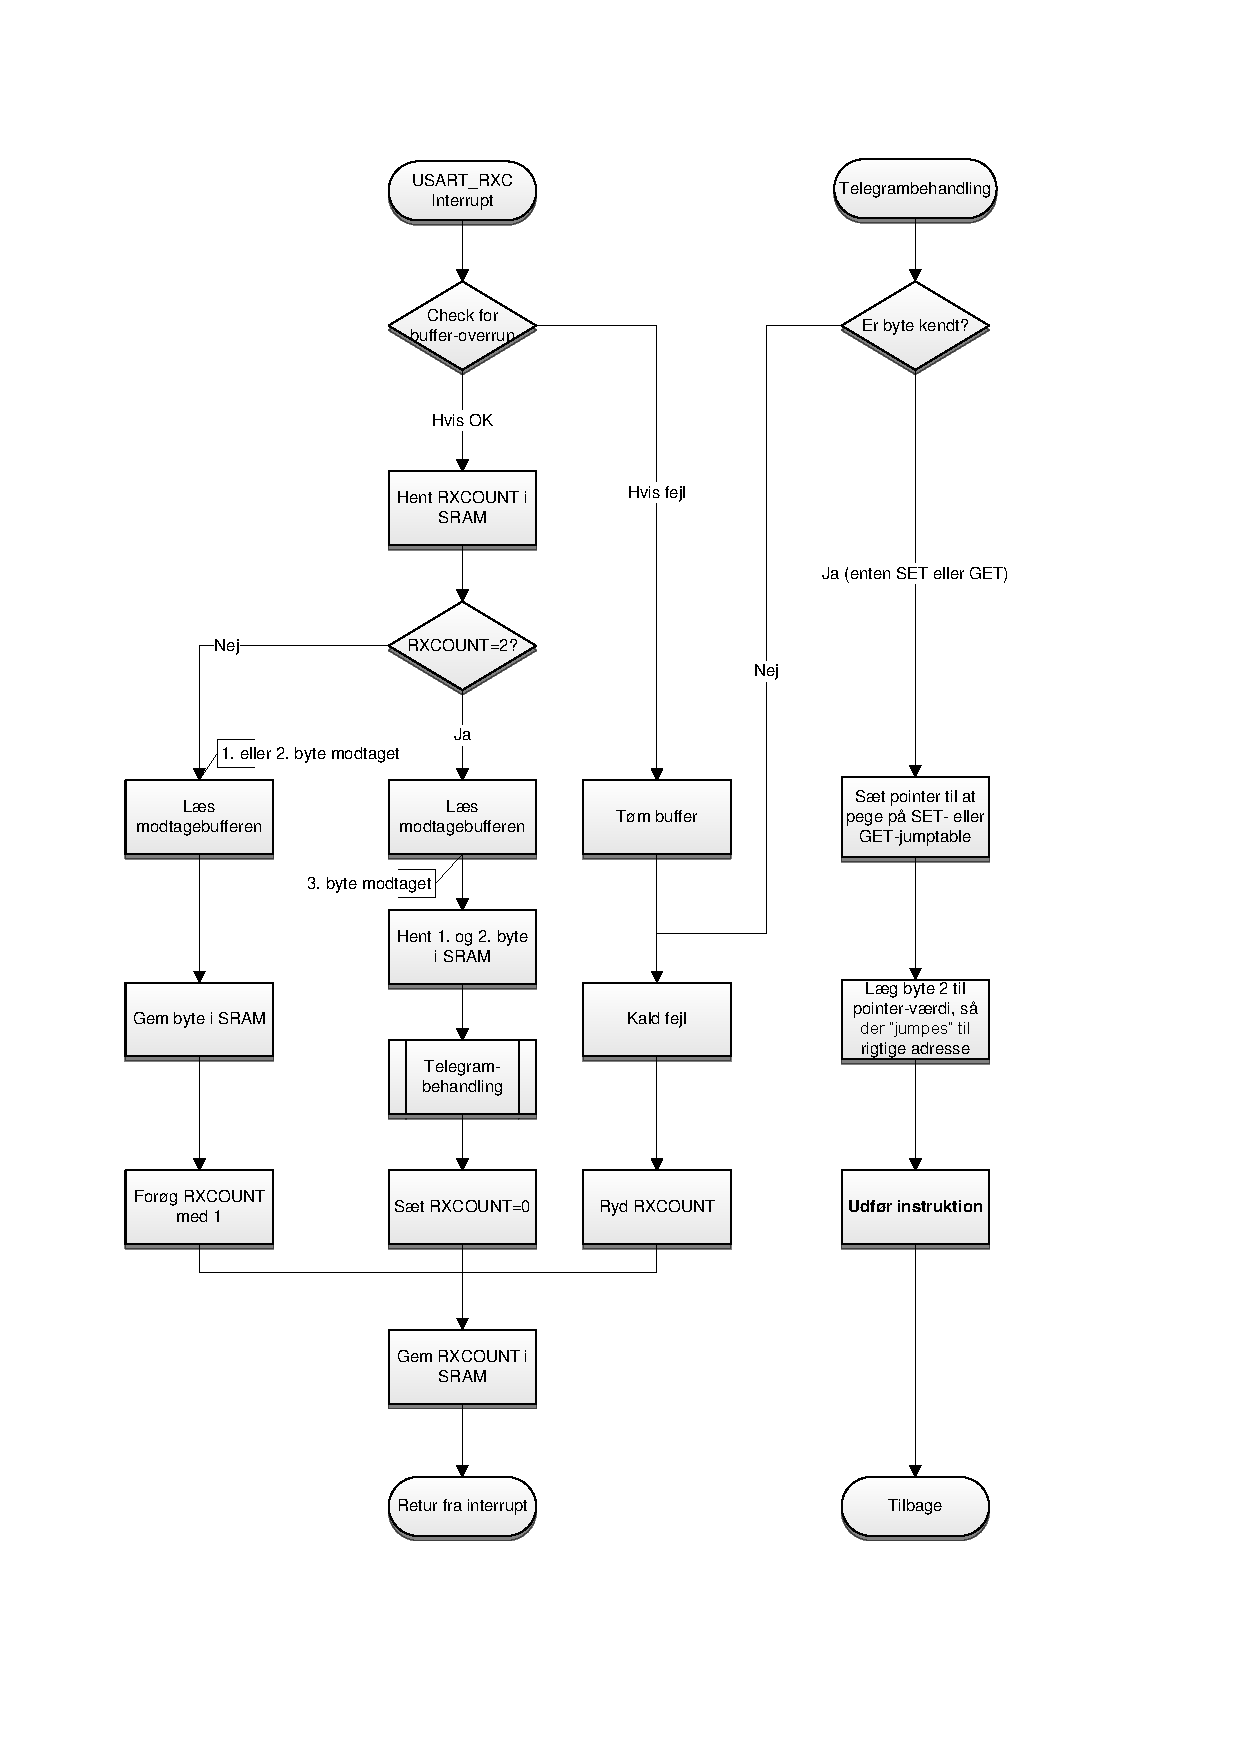
\includegraphics[page=1,scale=0.6,trim=113 96 123 80]{comms.pdf} %trim=l b r t
	\caption{USART Recieve Complete interrupt og behandling af telegram}
	\label{fig:usart_receive}
	\end{center}
\end{figure}

P� Figur \ref{fig:usart_receive} ses et diagram over USART Receive Complete interruptrutinen, som udf�res hver gang, der er ul�st data i \verb@UDR@ bufferen. De to f�rste bytes, der bliver modtaget i en r�kke, gemmes i hukommelsen, og s� snart den tredje modtages, udf�res den instruktion, telegrammet giver. Hvis ikke rutinen kender den, eller de bytes, der bliver modtaget, meldes der fejl, og t�lleren bliver sat tilbage til sin oprindelige v�rdi (0). Det giver mulighed for at kunne sende et nyt telegram allerede ganske kort tid efter, da koden ''redder sig selv''. I tilf�lde af modtagebuffer \textit{overrun} - alts� at den modtager data hurtigere end det kan l�ses - s�rger koden selv for at t�mme bufferen s�ledes at normal funktion kan genoprettes.

Den \textit{jump table}, der er n�vnt under telegrambehandlingsfunktionen i Figur \ref{fig:usart_receive} er en effektiv m�de at \textit{branche} til et andet sted i programmet p�. I stedet for at lade programmet l�be igennem en lang liste af \verb@cpi@\footnote{ComPare with Immidiate} instruktioner og sammenligne med hver enkelt byte, der repr�senterer en kommando, den skal kende, kan man lade den anden byte i telegrammet fungere som et off-set fra et kendt sted i programhukommelsen. En s�dan kendt adresse kunne v�re \verb@RX_SET_EVENTS@ (assembleren erstatter den \textit{label} med en faktisk adresse i programhukommelsen) som er vist i Programkode \ref{code:rxjump}.

\begin{lstlisting}[caption={RX SET EVENTS jump table},label={code:rxjump}]
RX_SET_EVENTS:
	rjmp	USART_RXC_Exec_ErrorByte2		;Byte 2 bestemmer off-set fra RX_SET_EVENTS
	rjmp	SET_MEM_LO						;01
	rjmp	SET_MEM_HI						;02
	rjmp	SET_MEM_Write					;03
	rjmp	USART_RXC_Exec_ErrorByte2		;04
	rjmp	SET_WD_Reset					;05
	rjmp	USART_RXC_Exec_ErrorByte2		;06
	rjmp	USART_RXC_Exec_ErrorByte2		;07
	rjmp	USART_RXC_Exec_Exit				;08
	rjmp	SET_Reverse						;09
	rjmp	USART_RXC_Exec_ErrorByte2		;0A
	rjmp	USART_RXC_Exec_ErrorByte2		;0B
	rjmp	USART_RXC_Exec_ErrorByte2		;0C
	rjmp	USART_RXC_Exec_ErrorByte2		;0D
	rjmp	USART_RXC_Exec_ErrorByte2		;0E
	rjmp	USART_RXC_Exec_ErrorByte2		;0F
	rjmp	SET_Start						;10
	rjmp	SET_Stop						;11
	rjmp	SET_ModeAuto					;12
	rjmp	SET_ModeDefault					;13
\end{lstlisting}

Et telegram best�ende af 0x55 (SET), 0x10 (Start) og 0xFF (Hastighed) ville lande p� adressen \verb@RX_SET_EVENTS@ + 0x10 og blive bedt om at \textit{branche} til \verb@SET_Start@, som findes et andet sted i programhukommelsen. Her vil de instruktioner, der f�r bilen til at k�re fremad, s� udf�res.

\subsubsection{Afsendelse}
USART'ens sendebuffer har plads til en byte. Skifteregistret fungerer som et 2. bufferniveau. Det vil sige, at er bufferen ledig, kan der flyttes to bytes ind i bufferen umiddelbart efter hinanden. Problemet opst�r, n�r en tredje byte skal skrives ind i \verb@UDR@ registret - hvis ikke man venter, til bufferen er tom, overskriver man den byte, der allerede ligger i bufferen og venter p� at blive flyttet ud. Umiddelbart kan man godt bare lade koden vente, til bufferen er blevet tom, men det er ikke �nskeligt, da det tager forholdsvis meget tid. Med en baud rate p� 9600 bit/s og en sending p� 10 bits (8 data bit, 1 start bit og 1 stop bit) per byte, der skrives til \verb@UDR@ registret, tager det omtrent et millisekund at sende en byte. Det vil sige, at skulle men bremse koden indtil alle tre bytes er sendt, er det meget sandsynligt, at der i hvert tilf�lde bliver spildt 16000 clock cycles.

L�sningen p� det problem er en tre byte stor buffer i microcontrollerens SRAM, som kan lagre en, to eller alle tre bytes af det telegram, der �nskes sendt - afh�ngig af hvorn�r bufferen bliver fuld. Man kan naturligvis stadig n� at fylde b�de USART bufferen \textit{og} bufferen i hukommelsen, men fordi microcontrolleren kun skal bruge sendefunktionen, n�r det kr�ves svar p� et GET-telegram, er det ikke sandsynligt, at det sker.

\begin{figure}[htb]
	\begin{center}
	\includegraphics[page=2,scale=0.6,trim=113 46 123 50]{comms.pdf} %trim=l b r t
	\caption{UsartTx funktionen og \textit{buffer empty} interruptrutinen}
	\label{fig:usart_transmit}
	\end{center}
\end{figure}

Figur \ref{fig:usart_transmit} viser funktionen UsartTx, som bliver kaldt, n�r microcontrolleren skal sende svar p� et GET-telegram. Argumenter til funktionen er de tre bytes, der �nskes sendt. UsartTx bruger en t�ller, TXCOUNT, der holder styr p�, hvilken byte i r�kken af tre den er n�et til. S� l�nge bufferen er klar til at modtage data, dvs. n�r \verb@UDRE@ flaget er sat, sendes der p� normal vis ved at skrive til \verb@UDR@ I/O registret. Hvis bufferen til geng�ld er fuld, gemmes den, eller de ikke-sendte bytes i SRAM og derefter sl�r UsartTx et interrupt til, der udl�ses, s� snart bufferen igen bliver klar til at modtage data. Interruptrutinen s�rger for at sende den n�ste byte, som den l�ser i SRAM i r�kken. P� den m�de muligg�res udf�relsen af andre instruktioner i microcontrolleren, selvom den er blevet bedt om at sende et REPLY-telegram.



\newpage
\section{Diskussion}
Valget af ADNS-9500 til afstandsm�ling var et modigt valg, da gruppen fra start var klar over, at det var en sv�r l�sning. Forventningen var, at opn� en h�jere pr�cision end med andre l�sningsmetoder. Da ADNS-9500 sensoren f�rst blev testet, p� et Arduino udviklingsboard, virkede kommunikationen uden problemer. Samspillet med Assemblerkoden p� ATmega32 microcontrolleren endte dog med at give problemer. Opstart, firmwareupload og umiddelbare tests forl�b problemtfrit, men efter nogen tid mistedes kommunikationen med sensoren. �rsagen til fejlen er stadig ikke opdaget: Det eneste f�lles for fejlene har v�ret, at de er opst�et mellem 20 sekunder og 5 minutter efter opstart af sensoren, hvilket har gjort fejls�gning sv�r.

Der har under test v�ret indikationer p�, at str�mmen kort afbrydes n�r bilen krydser overgangen mellem to banestykker. Det har givet sig til udtryk ved, at forbindelsen med bluetooth modulet er blevet afbrudt, og forbindelsen til det forbundede terminalprogram dermed ogs� er blevet afbrudt, imens at microcontrolleren har fortsat uafbrudt. Hvis str�mforsyningen i bilen er ustabil, kan dette have haft indflydelse p� den anvendte musesensor.

En alternativ l�sning til musesensoren kunne have v�ret en rotationsenkoder. Denne ville have v�ret lettere at implementere, da man kunne have undg�et at anvende SPI kommunikation. En rotationsenkoder er ikke blevet brugt, da en l�sning p� problemerne med ADNS-9500 sensoreren hele tiden har syntes at v�re indenfor r�kkevidde.

Projektet vil kunne udvides med en elektromagnet, hvorved der muligvis vil kunne opn�s en st�rre hastighed i sving. Den mulighed er dog ikke blevet forfulgt, da det har v�ret gruppens vudering, at det var vigtigere, at optimere softwaren til k�rsel af bilen.


%ADNS fejls�gnings har givet lille tid til optimering af k�rsel - rotationsenkoder ville m�ske ha v�ret bedre at have samtidig s� test kunne udf�res tidligere

%Assembler vs C = lang tid brugt p� kode debug / skrive simple prorgammer

%hardware SPI/interrupt prioritering = �get pr�cision p� ADNS

%Man kan monitorere bilens energiforbrug og virkningsgrad, baseret p� m�lt hastighed og acceleration(kraft) vs. m�lt elektrisk energiforbrug.

%At der laves en teoretisk (matematisk) model af bilens k�rsel p� banen, hvor-ved det skal v�re muligt at lave en teoretisk bedste gennemk�rsel (p� bag-grund af forskellige parametre, der afh�nger af bilens og banens egenska-ber), der s� kan sammenlignes med den bedste tid, der faktisk opn�s.

%ADNS kan detektere velocity sidel�ns

%regulering af hastighed 

%st�rre, software FIFO, sendebuffer?
\section{Konklusion} 
Ved hj�lp af accelerometeret har det v�ret muligt at m�le udslag i sving og ved tilpasning af afkoblingskondensatorer har st�j kunne minimeres. Softwaren har gjort at en mere pr�cis detektering har kunne opn�s, idet fejlagtige m�linger er sorteret fra.

Optosensoren er brugt til at registrere, hvorn�r bilen passerer m�lstregen. Kredsl�bet til optosensoren har fungeret tilfredsstillende og ved hj�lp af en tidsforsinkelse har det kunne sikres, at den ikke registerer m�lstregen flere gange ved samme passage.

Kommunikationen med musesensoren (ADNS-9500) har vist sig at virke, men en periodisk fejl, hvor sensoren ikke l�ngere sender korrekt data, har gjort k�rsel efter opm�lt data umulig. Hele ideen bag opm�lt k�rsel bygger p�, at bilens position altid er kendt. Det har derfor ikke v�ret muligt at teste koden, der bruges i forbindelse med k�rsel efter indsamlet data, i praksis.

Registreringen af sving har dog vist sig at v�re en succes, p� trods af, at positionsv�rdierne ofte har v�ret ukorrekte. Kommunikationsprotokollen har liges� fungeret godt og har, som det var meningen, muliggjort datalogging fra f. eks. accelerometer og musesensor. Samtidig har kommunikationsprotokollen lettet debugging.

H-broen er testet og virker efter hensigten. Hvis der laves fuld reversering, reduceres bremsel�ngden betydeligt. 
 
Der er designet et SMD print til ADNS9500 sensoren og det har gjort en optimal montering under bilen mulig.

Samlet set kan det konkluderes, at bilen ikke kunne k�re efter logget data. Udover afstandsm�ling har opsamling af de �vrige data virket efter hensigten. 





%%Litteratur
\newpage\thispagestyle{plain}

\nocite{*} % Inkluderer alle poster i bibl.bib-filen (dvs. kun skriv litteratur ind vi rent faktisk har brugt)
\printbibliography[title=Litteratur]\thispagestyle{plain}
\addcontentsline{toc}{section}{Litteratur}

\pagestyle{plain}%lidt pagestyle haxx




%%BILAG
\appendix

\newpage
\section{Hastighedsm�ling}\label{sec:bilag_hastighed}
Form�let med fors�get er, at finde en musesensor der vil kunne opfange bilens hastighed. For at finde ud af om musesensoren kan opfange bilens hastighed, m� nogle fors�g foretages. Hvis bilens maxhastighed er 6m/s, og den musesensor, der er tilt�nkt projektet, kun kan opfange 5m/s, m� en ny musesensor findes. For netop at finde den rigtige musesensor, m� disse fors�g derfor foretages.
\subsubsection*{Fors�gsopstilling}
\begin{figure}[htb]
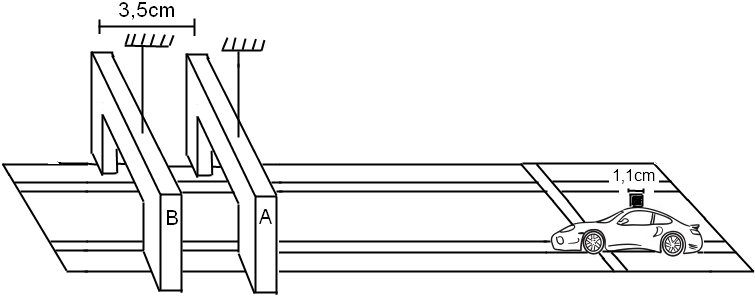
\includegraphics[scale=0.5]{hastighed3.png}
\caption{Hastighedsopstilling}
\label{hastighed}
\end{figure}
Bilen startes ved den hvide streg og f�r givet max hastighed. N�r bilen er i max hastighed, er en fotocelle opstillet, til at m�le dens hastighed. P� bilens tag er monteret en sort boks (som ses p� figur \ref{hastighed}). Fotocellen m�ler tiden det tager den sorte boks at pasere A, B og fra A til B (Kaldet AB). M�den hastigheden beregnes p�, er ved simpel matematisk udregning. Ved at tage et par fors�g og med tro p� at fotocellen fungere, kan dette fors�g siges at v�re fejlfrit. \\
F�lgende tabel er de seks fors�g, der er blevet udf�rt. 
\begin{table}[htb]
\begin{center}
	\begin{tabular}{| l | l | l | l|}
			\backslashbox{Fors�g}{Placering} & A (ms) & B (ms) & AB (ms)\\
			\hline
			1 & 2.68 & 2.60 & 85.91\\
			2 & 2.69 & 2.70 & 86.42\\
			3 & 2.55 & 2.58 & 82.27\\
			4 & 2.57 & 2.57 & 82.25\\
			5 & 2.53 & 2.50 & 80.83\\
			6 & 2.55 & 2.55 & 81.93\\
		\end{tabular}
\end{center}
	\caption{Hastighedsm�leresultater}
	\label{tab:hastighed} %%ref
\end{table} \\
Som tidligere n�vnt, kan hastigheden findes ved hj�lp af simple matematiske beregninger. Der er udvalgt tilf�ldigt i fors�gene og afstanden er delt med tiden. Det kan virke overfl�digt at tage seks udregninger med, men for at vise fors�gene n�sten er identiske, er dette alligevel valgt. 
\begin{align*}
Hastighed&=\frac{Afstand}{Tid} = \frac{1.1\cdot 10^{-2}m}{2.53 \cdot 10^{-3}s} = 4.35 \frac{m}{s}\\
Hastighed&=\frac{Afstand}{Tid} = \frac{1.1\cdot 10^{-2}m}{2.50 \cdot 10^{-3}s} = 4.40 \frac{m}{s}\\
Hastighed&=\frac{Afstand}{Tid} = \frac{1.1\cdot 10^{-2}m}{2.55 \cdot 10^{-3}s} = 4.31 \frac{m}{s}\\
Hastighed&=\frac{Afstand}{Tid} = \frac{350\cdot 10^{-3}m}{80.83 \cdot 10^{-3}s} = 4.33 \frac{m}{s}\\
Hastighed&=\frac{Afstand}{Tid} = \frac{350\cdot 10^{-3}m}{81.93 \cdot 10^{-3}s} = 4.27 \frac{m}{s}
\end{align*}
Fors�get er udf�rt uden top-karosset monteret p� bilen og bilen vil derfor aldrig kunne opn� denne max hastighed - da v�gten er betydelig mindre. Konklusionen p� dette fors�g er, at hvis musesensoren kan opfange mere end 4.40m/s, er det mere end rigeligt.

\newpage
\section{Metoder til afl�sning af ADNS sensor}\label{sec:bilag_adnsaflaesning}
Under udabejdelsen af programkoden til at hente data fra sensoren, blev forskellige l�sninger overvejet. Disse l�sninger er kort gennemg�et herunder.

\subsection{L�sning 1}
Denne l�sning blev valgt, og er beskrevet i detaljer i sektion \ref{sec:aflaesning_af_sensor}, hvorfor den ikke gennemg�s her.

\subsection{L�sning 2}
Denne l�sning er bygget op omkring at hele sensorafl�sningen sker i et timerinterupt. N�r timerinteruptet sker starter afl�sningen af sensoren, hvorefter hastighedsreguleringen startes. Fordelen ved denne er at den er forholdsvis simpel at implementere, og intervallet mellem afl�sning af sensoren vil v�re forholdsvis konstant. Problemet med denne model er, at denne model bruger rigtigt meget tid p� at vente p� svar fra sensoren, som ikke kan bruges til noget andet.

\begin{figure}[htb]
  \centering
  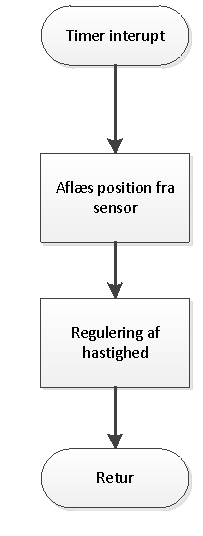
\includegraphics[scale=1]{ADNS_handling_met2.pdf}  
  \caption{Afl�sningsmetode 2}
  \label{fig:ADNS_handling_met2}
\end{figure}

\subsection{L�sning 3}
I denne l�sning afl�ses kun de to relevate data fra sensoren. Under start at microcontrolleren sendes foresp�rgsel om lav bytes en delta y v�rdien. N�r denne modtages, gemmes den, og der sendes foresp�rgsel om h�j byten af delta y. N�r delta y h�j modtages, gemmes denne og hastighedsreguleringen g�r i gang. Efter dette sendes foresp�rgsel om lav byte, og det hele starter forfra. Fordelen ved denne metode, er at der kun hentes data der skal benyttes. Detta kan ogs� se som v�rende en ulempe, da der derfor kun er disse til r�dighed ved fejlfindeing. Et problem med denne metode er at det ikke er muligt at verificere at det modtagede data er korrekt.

\begin{figure}[htb]
  \centering
  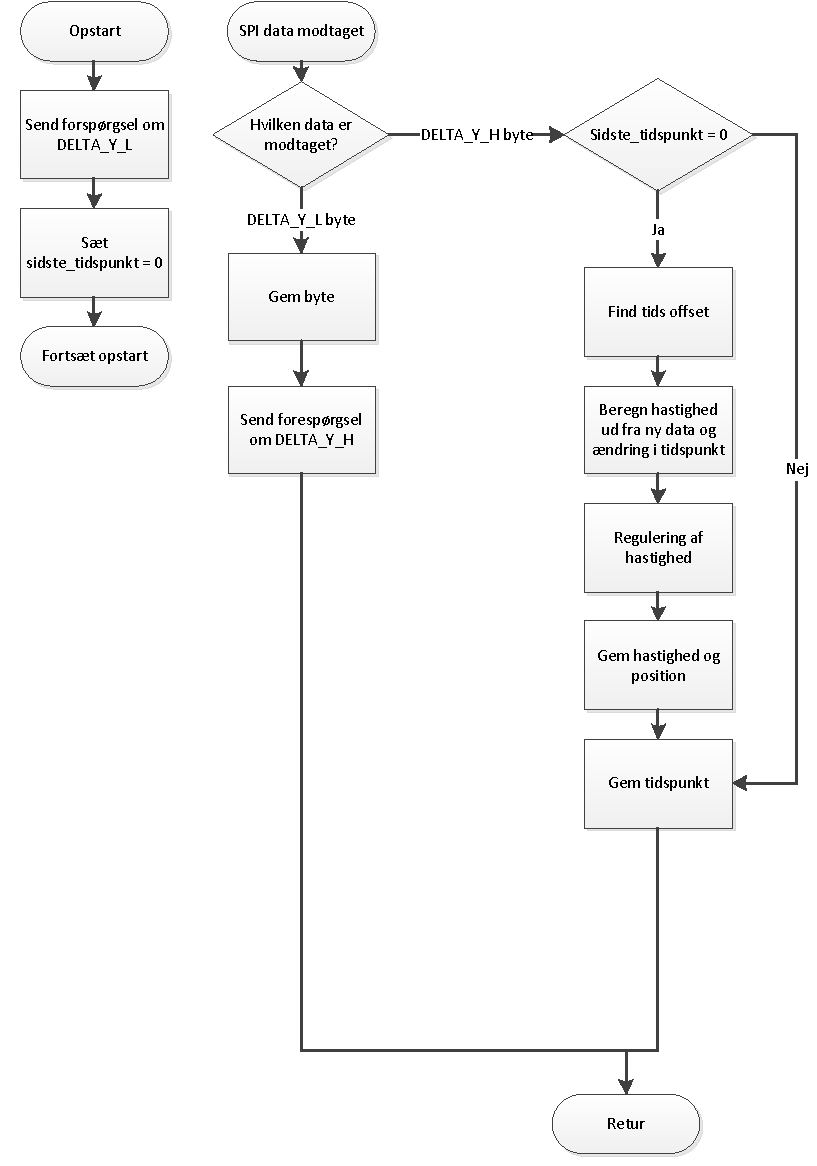
\includegraphics[scale=0.8]{ADNS_handling_met3.pdf}  
  \caption{Afl�sningsmetode 3}
  \label{fig:ADNS_handling_met3}
\end{figure}


\subsection{Begrundelse for valg}
%Umiddelbart er det i dette projekt kun relevant at 
%Det blev valgt at benytte l�sning 1, da der er en lang r�kke .... 

Til afhentning af data er l�sning 1 benyttet. Valget er truffet p� baggrund af, at denne model har en masse ekstra information fra sensoren. Dette ekstra info kan benyttes til at kontrollere, om sensoren rent faktisk er i en funktionel tilstand, og udfra dette kan der eventuelt senere opbygges programkode, der s�rger for at genstarte sensoren ved fejl under k�rslen. Ved at f.eks at have valgt l�sning to eller tre, ville en fejl i kommunikationen ikke opdages, og herved vil der ikke kunne tages h�jde for dette. Ved l�sning et er der mulighed for at kontrollere MOTION\footnote{V�rdi der viser sensorens tilstand}-og SQUAL\footnote{Surface Quality}-v�rdien fra sensoren, da disse giver et repr�sentativt billede af kvaliteten af de m�lte data og sensorens tilstand.

\newpage
\section{Accelerometer m�ling}\label{sec:bilag_acc}
Ved konstruering af et accelerometer er det vigtigt at montere den rette kondensator som afkobling. Ved de f�lgende fors�g er der monteret forskellige kondensator, og derefter er den data, microcontrolleren udsender, plottet som funktion af positionen. Banen, bilen k�rte p�, er vist p� Figur \ref{fig:bane}. Der er markeret ved tekstbokse fra A-D, som viser de forskellige sving. Disse kan derefter afl�ses p� de f�lgende grafer.

\begin{figure}[H]
	\begin{center}
	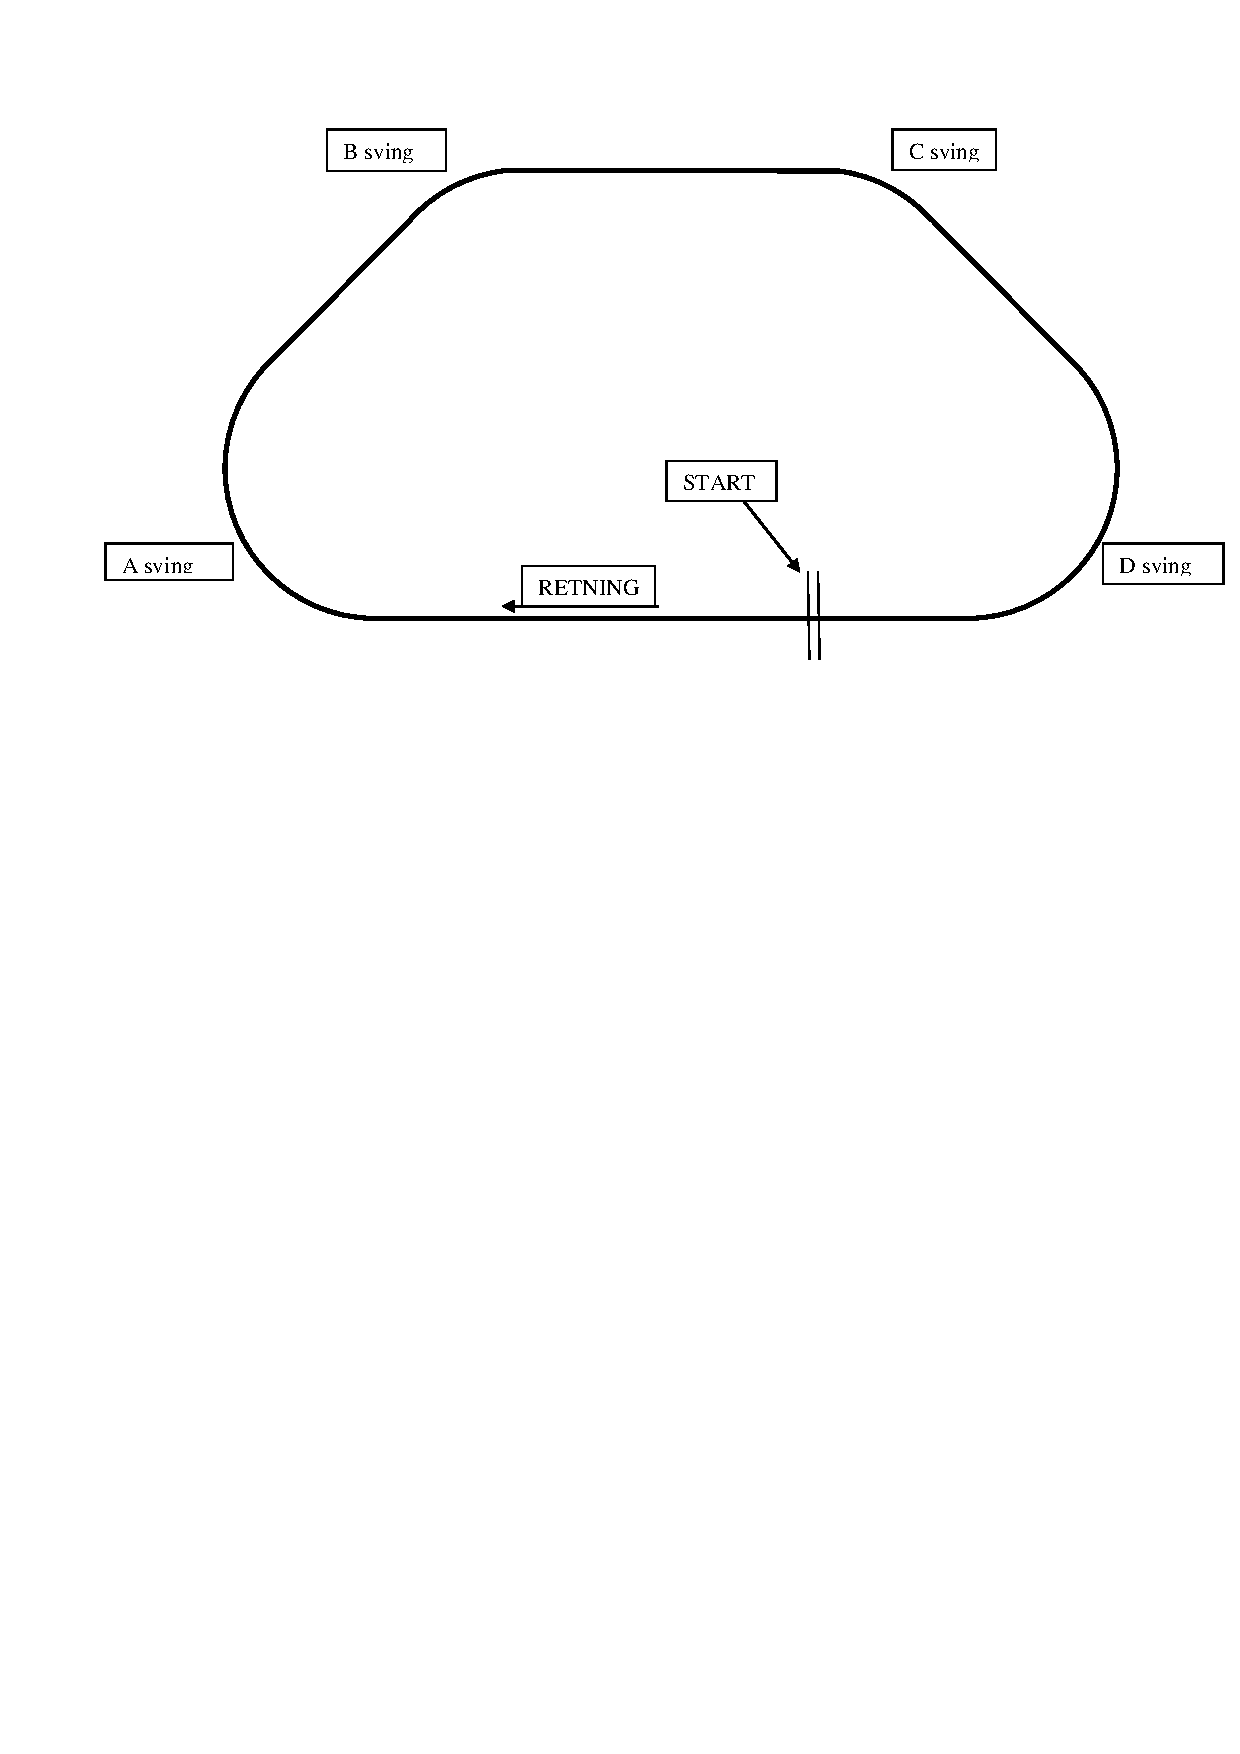
\includegraphics[scale=0.8,trim=40 520 0 50]{bane.pdf}%trim=l b r t
	\caption{Banen accelerometer-test blev udf�rt p�}
	\label{fig:bane}
	\end{center}
\end{figure}

Hvis ingen kondensator er monteret, er dataen accelerometeret sender ud, totalt ubrueligt. Derfor er der ikke tilf�jet A-D, da dataen er fuldst�ndig ubrugelig.  Det er vist p� Figur \ref{fig:acc0uftest0}, hvor bit-v�rdien er p� den lodrette akse og tiden er p� den vandrette akse.

\begin{figure}[H]
	\begin{center}
	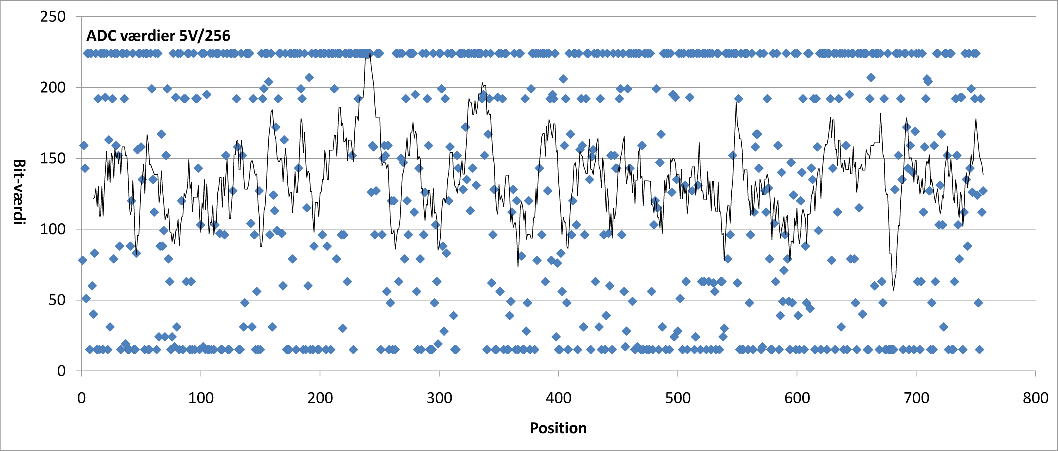
\includegraphics[scale=0.8]{acc_0uf_test0.pdf}%trim=l b r t
	\caption{Ingen kondensator monteret}
	\label{fig:acc0uftest0}
	\end{center}
\end{figure}

Der blev derefter monteret en 0,47$\mu$F kondensator og resultatet blev straks meget bedre - men stadig ikke tilfredsstillende. Man ser tydeligt, at den opfanger svingene, men stadig er mange v�rdier svingende. Dette ses p� Figur \ref{fig:acc_047uf_test2}

\begin{figure}[H]
	\begin{center}
	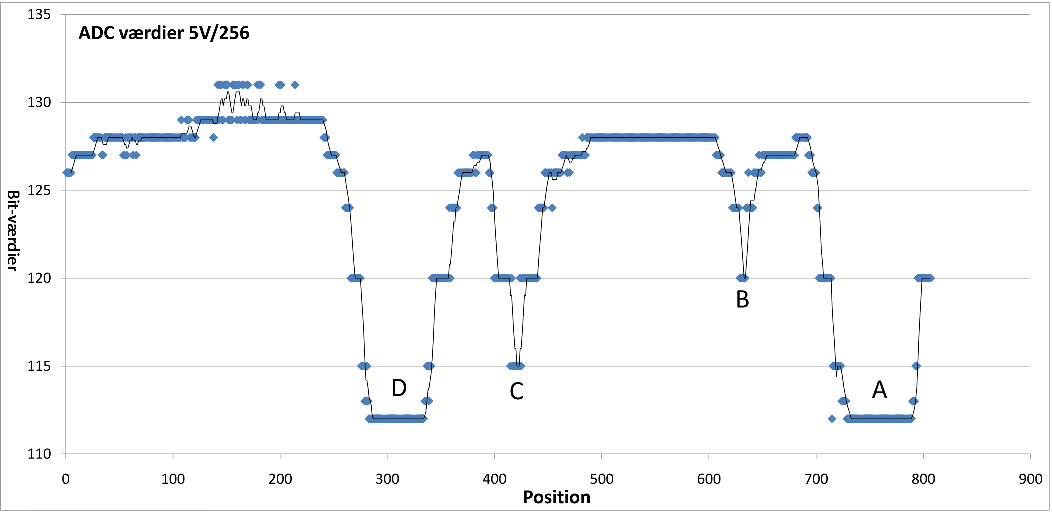
\includegraphics[scale=0.8]{acc_047uf_test2.pdf}%trim=l b r t
	\caption{0.47$\mu$F kondensator omvendt k�rsel}
	\label{fig:acc_047uf_test2}
	\end{center}
\end{figure}

For at kunne g�re m�lingerne mere pr�cise, m�tte en st�rre kondensator monteres som afkobling. Derfor blev en 1.0$\mu$F Kondensator monteret, og her blev resultatet rigtig godt. Som vist p� Figur \ref{fig:acc_1uf_test5}, ser man tydeligt, at alle sving bliver opfanget knivskarpt.

\begin{figure}[H]
	\begin{center}
	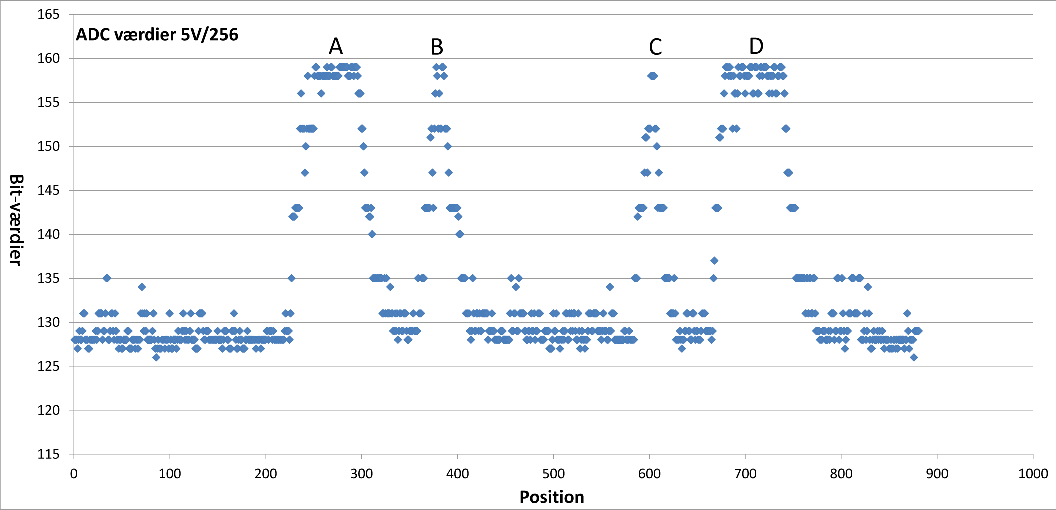
\includegraphics[scale=0.8]{acc_1uf_test5.pdf}%trim=l b r t
	\caption{1.0$\mu$F kondensator}
	\label{fig:acc_1uf_test5}
	\end{center}
\end{figure}

For at finde ud af om montering af en st�rre kondensator, ville give d�rligere eller bedre pr�cision, monteres der en 1.5$\mu$F kondensator. Som vist p� Figur \ref{fig:acc_1_5uf_test6} ses der, at resultaterne er rimelig pr�cise, men der bliver desv�rre sk�ret nogle af svingene af. Dette ses fx ved punkt C, der er sk�ret noget af acceleracionen af. Dette vil i sidste ende give store problemer. 

\begin{figure}[H]
	\begin{center}
	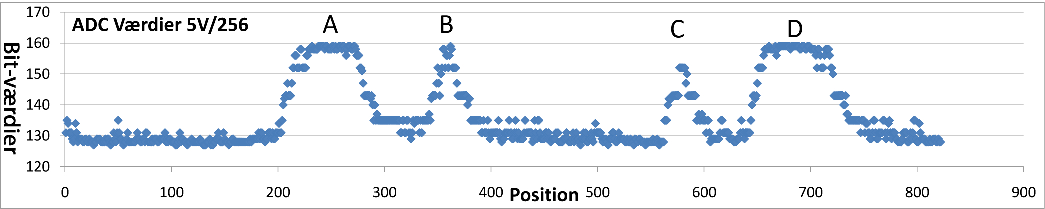
\includegraphics[scale=0.8]{acc_15uf_test6.pdf}%trim=l b r t
	\caption{1.5$\mu$F kondensator}
	\label{fig:acc_1_5uf_test6}
	\end{center}
\end{figure}

Som tidligere n�vnt blev 1.0$\mu$F den store vinder og derfor er denne monteret p� accelerometeret.

\newpage
\section{H-bro test}\label{sec:bilag_hbrotest}
For at p�vise, at H-broen fungerer til at �ge Scalextricbilens bremseevne, er der foretaget en r�kke fors�g. Som beskrevet i sektion \ref{sec:hbro}, er form�let med H-broen at bremse bilen. Hvor stor en kraft motoren skifter retning med, kan vha. microcontrolleren justeres alt efter hvilke v�rdier der sendes til bilen. Der sendes en hexadecimal v�rdi fra 0x00-0xFF til bilen, hvor 0x00 er ingen v�rdi og 0xFF er max bagud/forud-rettet kraft. 0x00 har ingen effekt p� bilen og den vil forts�tte up�virket. Des h�jere v�rdien s�ttes til, des st�rre kraft bremses bilen med. P� Figur \ref{fig:hbrotest} kan der ses de 3 bremsel�ngder med henholdsvis a0, kortslutning og fri l�b.

\begin{figure}[htb]
\center
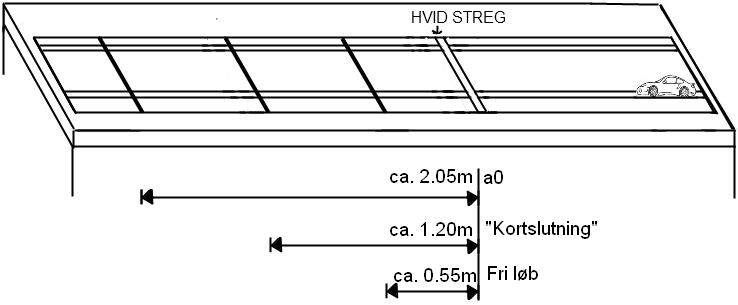
\includegraphics[scale=0.5]{hbrotest.png}
\caption{H-bro test}
\label{fig:hbrotest}
\end{figure}

Som der ses p� figuren, er der markeret en hvid streg p� skinnen, som optosensoren opfanger. N�r bilen passere denne streg t�ndes H-broen med den v�rdi der nu er sendt til den. Som tidligere n�vnt skifter motoren retning og hastigheden daler hurtigt. Efter kort tid vil bilen i et kort �jeblik st� stille og bakke. Netop dette �jeblik registreres med m�leb�nd og �jet. Udfra Figur \ref{fig:hbrotest} ses der at jo st�rre Hex V�rdi der sendes, jo kortere bremsel�ngde har bilen. Konklusionen p� dette fors�g er, at H-broen virker ubeklageligt. 

\newpage
\section{Komponentliste}\label{sec:komponent_liste}

F�lgende komponenter er blevet anvendt til konstruktion af:

\begin{table}[htb]
\begin{minipage}[b]{0.5\linewidth}
\begin{tabular}{l l l}
\multicolumn{3}{c}{H-bro} \\
\hline
Del & V�rdi/model & type\\
D1 & - & Diode\\
D2 & - & Diode\\
D3 & - & Diode\\
D4 & - & Diode\\
IC1 & L298 & H-bro\\
\end{tabular}
\end{minipage}
\begin{minipage}[b]{0.5\linewidth}
\begin{tabular}{l l l}
\multicolumn{3}{c}{Musesensor} \\
\hline
Del & V�rdi/model & type\\
C1 & 470pF & Kondensator\\
C2 & 100nF & Kondensator\\
C3 & 100nF & Kondensator\\
C4 & 10uF & Kondensator\\
C5 & 10nF & Kondensator\\
C6 & 1uF & Kondensator\\
C8 & 100nF & Kondensator\\
C9 & 10uF & Kondensator\\
C10 & 100nF & Kondensator\\
C11 & 4.7uF & Kondensator\\
C12 & 4.7uF & Kondensator\\
U\$1 & ADNS-9500A & Mussesensor\\ 
U\$2 & 2N5460 & Transistor\\
\end{tabular}
\end{minipage}
\end{table}

\begin{table}[htb]
\begin{minipage}[b]{0.5\linewidth}
\begin{tabular}{l l l}
\multicolumn{3}{c}{Accelerometer} \\
\hline
Del & V�rdi/model & type\\
C1 & 100nF & Kondensator\\
C2 & 1uF & Kondensator\\
C3 & 1uF & Kondensator\\
U\$1 & ADXL203 & Accelerometer\\
\end{tabular}
\end{minipage}
\begin{minipage}[b]{0.5\linewidth}
\begin{tabular}{l l l}
\multicolumn{3}{c}{Optocoupler} \\
\hline
OPTO & CNY70 & optocoupler\\
R1 & 180 & Modstand\\
R2 & 15K & Modstand\\
\end{tabular}
\end{minipage}
\end{table}

\newpage
\section{CD indhold}\label{sec:cdindhold}
Her findes en liste over indholdet p� den vedlagte CD i tr�-struktur. Kommentarer beskriver indholdet af udvalgte mapper, hvor ikke alle enkeltst�ende filer er oplistet.

\dirtree{%
.1 /.
	.2 Accmetertest.
		.3 Accmeter\_tests.xlsx\DTcomment{M�leresultater fra tests med acc. meter (App. \ref{sec:bilag_acc})}.
	.2 Datablade\DTcomment{Datablade for de benyttede sensorer}.
	.2 Kildekode\DTcomment{Samlet Assembler kildekode brugt i projektet}.
		.3 adns9500.
	.2 Kommunikationsprot.
		.3 Fejlkoder.pdf\DTcomment{Fejlkoder sendt af Error() funktionen: Til debugging}.
		.3 Kommunikationsprotokol.pdf\DTcomment{Kommandoer, som programmet reagerer p�}.
	.2 Litteratur.
		.3 The optical mouse as a two-dimensional displacement sensor.pdf.
	.2 M�der\DTcomment{M�dedagsordener og referater}.
	.2 Rapport\_Latex\DTcomment{LaTeX kildefiler}.
		.3 graphics\DTcomment{Grafik brugt i rapporten}.
	.2 Tidsplaner.
		.3 Tidsplan\_overordnet.pdf.
		.3 Tidsplan\_Sidste3uger.pdf.
	.2 Midsvejspraesentation.pptx.
}

%%SOURCECODE
%\newpage
%\section{Kildekode}
%
%\lstinputlisting[captionpos=t,title=\lstname]{./sourcecode/root/main.asm}
%\lstinputlisting[captionpos=t,title=\lstname]{./sourcecode/root/macros.asm}
%\lstinputlisting[captionpos=t,title=\lstname]{./sourcecode/root/adns9500/adns_spi.asm}
%\lstinputlisting[captionpos=t,title=\lstname]{./sourcecode/root/adns9500/adns_aux.asm}
%\lstinputlisting[captionpos=t,title=\lstname]{./sourcecode/root/adns9500/adns_run.asm}
%\lstinputlisting[captionpos=t,title=\lstname]{./sourcecode/root/speedcalculation.asm}
%\lstinputlisting[captionpos=t,title=\lstname]{./sourcecode/root/interrupts.asm}
%\lstinputlisting[captionpos=t,title=\lstname]{./sourcecode/root/ana_comp.asm}
%\lstinputlisting[captionpos=t,title=\lstname]{./sourcecode/root/comm.asm}
%\lstinputlisting[captionpos=t,title=\lstname]{./sourcecode/root/commactions.asm}
%\lstinputlisting[captionpos=t,title=\lstname]{./sourcecode/root/utils.asm}
%\lstinputlisting[captionpos=t,title=\lstname]{./sourcecode/root/debug.asm}
%\lstinputlisting[captionpos=t,title=\lstname]{./sourcecode/root/ModeDefault.asm}
%\lstinputlisting[captionpos=t,title=\lstname]{./sourcecode/root/ModePreWarmup.asm}
%\lstinputlisting[captionpos=t,title=\lstname]{./sourcecode/root/ModeWarmup.asm}
%\lstinputlisting[captionpos=t,title=\lstname]{./sourcecode/root/ModeRace.asm}
%\lstinputlisting[captionpos=t,title=\lstname]{./sourcecode/root/ModePreRace.asm}
%\lstinputlisting[captionpos=t,title=\lstname]{./sourcecode/root/adns9500/adns_firmware.asm}   % <- skal m�ske undlades ^^


\end{document}